\documentclass[12pt,a4paper]{report}
\usepackage{ADG}
% \usepackage[margin=1in]{geometry}
\usepackage{cite}
\usepackage{listings}
\usepackage{xcolor}
\usepackage{color}
\usepackage{tabularx}
\usepackage{booktabs}
\usepackage{graphicx}
\usepackage{float}
\usepackage{enumitem}
\setlist[itemize]{noitemsep, topsep=0pt}
\usepackage{tikz}
\usepackage{tikz-uml}
\usepackage{pdflscape}
\usepackage{longtable}
\usepackage{array}
\usepackage{ragged2e}
\usepackage{pgfplots}
\pgfplotsset{compat=1.18}
\usepackage{caption}
\usepackage{subcaption}
\usepackage{csvsimple}
\usepackage{textcomp}
\usepackage{pgfgantt}

\definecolor{lightgray}{gray}{0.95}

\tikzset{
	umlinclude/.style={pos=0.6, below},
	umlassoc/.style={pos=0.5, below}
}

\lstset{
	breaklines=true,
	breakatwhitespace=false,
	postbreak=\mbox{\textcolor{red}{$\hookrightarrow$}\space},
	basicstyle=\ttfamily,
	backgroundcolor=\color{lightgray},
	keywordstyle=\color{blue},
	commentstyle=\color{gray},
	stringstyle=\color{red},
	numberstyle=\color{orange}
	columns=fullflexible,
	extendedchars=true,
	keepspaces=true,
	showspaces=false,
	showstringspaces=false,
	language=C++,
}

\begin{document}

\thispagestyle{empty}
%temporarily set the line height to 1.0
{\setstretch{1.0}

\noindent
\includegraphics[scale=0.32]{images/euc.jpg}


\begin{center}
 School of Sciences \textbar \; Department of Computer Science and Engineering
\end{center}

\vspace{1.5cm}
\begin{center}
\Huge  [enter the project title here]
\end{center}


\vspace{0.2cm}
\begin{center}
\Large [enter any applicable subtitle here]
\end{center}

\vspace{1.5cm}
\begin{center}\LARGE Bachelor of Science in [enter your discipline here]
\end{center}


\vspace{1.5cm}
\begin{center}
\Large [enter your name here]
\end{center}
\vspace{1.5cm}

\noindent
\begin{center}\copyright  [month year]
\end{center}
\newpage
\thispagestyle{empty}

}%setstrech{1.0}

\section*{Acknowledgements}
\addcontentsline{toc}{chapter}{Acknowledgements}
I would like to express my gratitude to my supervisor, Dr. Konstantinos Katzis, for his constant encouragement, technical guidance, and enlightening critique during this project. His advice was extremely useful to me as I navigated the technical and conceptual challenges of creating a reliable embedded healthcare system, particularly given the fact that this was my first experience with electronics design and construction.

I also want to express my gratitude to my panellist, Dr. Costas Iordanou, for his careful review of this report and his insightful suggestions, which significantly improved its clarity and thoroughness.

\newpage
\section*{Abstract}
\addcontentsline{toc}{chapter}{Abstract}
In order to ensure patient safety and detect issues early, it is essential to monitor the patient's vital signs during the post-operative phase. The design and implementation of an Internet of Things (IoT)-based monitoring system that can gather vital sign data from commercially available medical sensors with Bluetooth capabilities and send important readings to the cloud via the LoRaWAN communication protocol is presented in this thesis. The system incorporates a 16x2 LCD, tactile buttons, LED indicators, a buzzer for multimodal feedback, all driven by a custom menu-driven user interface. It is built on an Arduino-compatible device.

The behaviour of the device is controlled by a finite state machine (FSM), which enables reliable state changes depending on sensor data, human input, and Bluetooth communication status. Out-of-range data is sent automatically to a remote monitoring platform according to preset conditions, and readings are verified and evaluated against user-configured thresholds. To test the system in a variety of realistic scenarios and replicate sensor data, an accompanying mobile application was developed. Remote control, data logging, and cloud-based alerting were made possible through integration with TagoIO and The Things Network (TTN).

The prototype showed reliable collection of data, threshold evaluation, and error handling during the implementation and testing stages. This work offers a post-operative care solution that is scalable, power-efficient, and adaptable, even in environments without easy access to hospital infrastructure such as remote rural locations. Issues including managing Bluetooth disconnections and integrating proprietary sensors are examined, along with potential solutions.
\newpage
%temporarily set the line height to 1.0
{\setstretch{1.0}
\tableofcontents
}


\chapter{Introduction}

\section{Introduction} % Section 1.1
It is crucial to monitor patient vital signs in the post-operative period to ensure detection of any complications early on, and increase patient safety. Traditionally, nurses and clinical staff carry out this monitoring at regular intervals, which may leave gaps in observation and increase the risk of missing early warning signs. Advances in the Internet of Things (IoT) space have created new possibilities for real-time, continuous monitoring of patients using wireless sensors and communication protocols.

One of the main difficulties in implementing IoT systems in healthcare is selecting appropriate technologies for communication, that balance power consumption, range, and reliability, at a reasonable cost. Bluetooth, which is a widely used technology in consumer health devices, offers short-range, low-energy connectivity but it doesn't scale well to the sizsize of a hospital, for the purpose of monitoring hundreds of patients at a time. LoRaWAN on the other hand, is capable of communication at long ranges, using low power to transmit small amounts of data (perfect for sending the kinds of data sensors produce) from multiple devices to a central gateway.

This thesis presents the design and implementation of a device intended for the purpose of monitoring patient vital signs in the post-operative context, that integrates consumer medical sensing devices, and incorporates both Bluetooth as well as the LoRaWAN communication protocols. It is designed to collect data from commercially available medical devices and send that data efficiently to the cloud for analysis and alerting purposes.

\section{Aims and Objectives} % Section 1.2
The main aim of this project is to design and develop an IoT based device to monitor post-operative vital signs. Several specific aims were defined, with clear objectives for each:
\begin{enumerate}
	\item Investigate the clinical requirements and difficulties in the context of post-operative vital sign monitoring.
	\begin{itemize}
		\item Conduct a literature review on the importance of post-operative monitoring.
		\item Conduct a literature review on the clinical importance of each vital sign in the post-operative context.
	\end{itemize}
	\item Evaluate and compare appropriate commercially available Bluetooth capable medical devices for possible integration with the system.
	\begin{itemize}
		\item Identify commercially avaialble Bluetooth capable devices for measuring temperature, blood pressure, and heart rate.
		\item Assess their Bluetooth connectivity and opennes, and as such determine their likely degree of integration with a custom system such as the one being developed.
	\end{itemize}
	\item Analyse and select suitable communication technologies for device integration and data transmission to cloud.
	\begin{itemize}
		\item Review relevant communication protocols for device integration.
		\item Review relevant communication protocols for long range data transmission to the cloud.
		\item Justify the selection of technologies to be used in the system.
	\end{itemize}
	\item Design and implement an IoT system to monitor vital signs post-operation.
	\begin{itemize}
		\item Develop the system architecture, consisting of the device itself as well as a simple backend cloud platform.
		\item Make the device capable of connecting to and communicating with Bluetooth devices such as medical sensors.
		\item Establish communication between the device itself and the backend cloud platform using LoRaWAN.
	\end{itemize}
	\item Test the system under realistic conditions and evaluate its performance.
	\begin{itemize}
		\item Conduct testing of the system with simulated data representing data incoming from a medical sensor, and test transmission via the LoRaWAN protocol to the cloud.
		\item Evaluate metrics such as data reliability, scalability, and energy efficiency.
	\end{itemize}
	\item Analyse the project outcomes and propose possible future improvements.
	\begin{itemize}
		\item Discuss strengths, weaknesses, and potential points of improvement of the system.
		\item Discuss any challenges or difficulties faced during design and development.
		\item Suggest possible further research and enhancements.
	\end{itemize}
\end{enumerate}

\section{Structure of the thesis} % Section 1.3
This thesis is organised into six main chapters, following the natural development process (starting with research and design, followed by implementation, ending with an analysis of the outcomes).

\begin{itemize}
	\item \textbf{Chapter 1: Introduction} --- Introduces the background, aims, objectives, and structure of the thesis.
	\item \textbf{Chapter 2: Background or Project Scope} --- Reviews the clinical significance of monitoring vital signs after surgery, the role of IoT in this task, analyses current communication protocols and available medical sensing devices, and discusses some points of consideration regarding integration of said devices with the system.
	\item \textbf{Chapter 3: Analysis and Design} --- Describes the 'user needs', requirements analysis, system architecture, detailed design of the system, and gives reasons for design desisions that were made.
	\item \textbf{Chapter 4: Implementation and Testing} --- Presents the implementation of features, implementation of communication with backend cloud via LoRaWAN, and testing procedures.
	\item \textbf{Chapter 5: Discussion} --- Discusses the resulting system, difficulties encountered, lessons learned, and possible improvements.
	\item \textbf{Chapter 6: Bibliography} --- Lists all the references cited throughout the thesis.
\end{itemize}

\section{Summary} % Section 1.4
This chapter gave an introduction to the reasoning behind developing such an IoT based system for the post-operative scenario, gave an outline for the aims and objectives of the project, and briefly covered the general structure of the thesis. The next chapter will dive deeper into the background of the project including clinical signigicance of vital sign monitoring, the role of IoT, relevant communication protocols, and compare and evaluate commercially available Bluetooth-capable medical sensing devices for this project.


\chapter{Background}

\section{Introduction} % Section 2.1
The healing process does not end after surgery is complete, but instead it is often a long effort for weeks or months post-operation. Furthermore, it is not just the physical health of the patient which must be considered, but also and perhaps equally important their mental health and quality of life moving forward. In recent decades it has become clearer to medical professionals that extended monitoring following operations greatly impacts the results of surgeries in a positive manner, as stated in \cite{d2014defining}. Of course, there are multiple factors affecting the extent to which complications will arise in a patient after receiving surgery, such as their age, previous health issues, or conditions which may develop in parallel to the primary diagnosis even if they are in fact unrelated. In particular, the elderly are quite vulnerable to more complications, as stated by the authors in \cite{kare2024post}, specifically referring to elderly patients who underwent hip fracture surgery. Such complications affect quality of life longterm as well as general ability to function normally, not just physical health, degree of recovery, and survivability \cite{kare2024post}.

The role of the surgeon in the postoperative context is to firstly make sure the patient is receiving the necessary support to sustain a healthy balance in their body, and do whatever they can to avoid the development of any complications that may appear as a result of the procedure. Should any complications arise despite the medical staff's best efforts, it is then the surgeon's responsibility to recognise the signs pointing to the development of said complications and take appropriate actions to quickly and effectively manage them, allowing the patient to recover to their preoperative state eventually \cite{Surwit_Tam_2008}

\section{Clinical significance of monitoring each vital sign post-surgery} % Section 2.2
% Vital signs give a rich picture of patient condition post surgery, providing medical staff with the information required to adequately care for the patient. Different measurements have varying significance depending on the stage of recovery the patient finds themselves in, however they should be continuously measured to provide history and an indication of trends to clearly show the progress of the patient's condition. Immediately after surgery measurements must be taken often as that is the most critical stage of the recovery process. In the beginning, vitals such as respiratory rate and blood pressure are vastly more important due to their indication of how the patient is recovering from anesthesia, but once they sufficiently recover from it pulse rate is a better indicator of the volume of blood in the circulatory system of a patient \cite{Surwit_Tam_2008}.

Postoperative vital sign monitoring is essential for both patient safety and the early identification of problems. Specific information on the patient's physiological state and course of recovery is provided by each measure.

\textbf{Blood Pressure}

To detect hypotension or hypertension, which can both result in major problems, postoperative blood pressure monitoring is crucial \cite{Kachel2021_pb}. By enabling early diagnosis and control of blood pressure variations, continuous monitoring lowers the risk of postoperative haemorrhage and other unfavourable outcomes \cite{Demetz2024_pl}. Continuous monitoring, according to studies, can identify hypotensive events that intermittent measures could overlook, allowing for prompt responses \cite{Noto2024_uz}.

\textbf{Temperature}

After surgery, maintaining normothermia is essential to avoiding problems including surgical site infections and extended hospital stays. Hypothermia can raise the risk of infection and hinder the healing of wounds. Thus, it is advised to regularly check the patient's temperature during the postoperative phase in order to guarantee the best possible results \cite{Frank1999_rb}.

\textbf{Oxygen Saturation}

Monitoring oxygen saturation is essential for identifying hypoxaemia, which, if left untreated, can result in organ dysfunction. Early management in cases of respiratory compromise is made possible by pulse oximetry, which offers a non-invasive way to continuously measure oxygen levels. When compared to sporadic inspections, continuous monitoring has been demonstrated to improve the detection of oxygen desaturation \cite{Khanna2024_fz}.

\textbf{Heart Rate}

In the postoperative phase, heart rate monitoring is crucial for spotting physiological alterations that could indicate patient decline. As stated in \cite{Khanna2025_sg} heart rate changes, like bradycardia or tachycardia, can occur hours or even days before serious occurrences like cardiac arrest, particularly in the 48 hours after surgery. This emphasises the necessity of regular or ongoing monitoring. As is typical in many wards, manual spot checks conducted every 4–8 hours are not enough to accurately identify these occurrences. Continuous monitoring, on the other hand, has been demonstrated to detect heart rate anomalies more frequently and with greater severity than would otherwise be detected, enabling medical professionals to take early action and possibly avert problems or death \cite{Khanna2025_sg}.

\textbf{Respiratory Rate}

Since respiratory rate (RR) is a sensitive predictor of early physiological decline, it is clinically important to monitor RR in postoperative patients. According to studies, irregular RR frequently precedes changes in other vital signs like blood pressure or heart rate and is the first obvious indication of a patient's decline. In clinical settings, RR is commonly undermonitored despite its significance. Elliott \cite{Elliot2016Respiratory} pointed out that RR evaluation is frequently disregarded because of factors including a lack of automated measurement methods, time restrictions, and insufficient clinician understanding. This error raises the possibility of unfavourable outcomes by delaying the identification of respiratory impairment.

Furthermore, it has been demonstrated that ongoing respiratory rate (RR) monitoring improves patient safety during the recovery phase. In a retrospective observational analysis, patients who had laparoscopic colon surgery were contrasted with those who had conventional intermittent monitoring in terms of continuous RR monitoriing. Two life-threatening respiratory episodes occurred in the intermittently watched group (2 out of 126 patients), while none occurred in the continuously monitored group (0 out of 69 patients), according to the study. According to these results, ongoing RR monitoring may help identify respiratory depression early, enabling prompt treatment and better patient outcomes \cite{Kawanishi2017Incidence}.

It is crucial to remember that the type of operation done and the patient's unique risk factors can affect each vital sign's clinical significance. In order to solve this, the suggested system offers vital sign threshold customisation, allowing medical professionals to adjust monitoring settings to the unique requirements of every patient and surgical situation.

\section{Role of IoT in vital sign monitoring} % Section 2.3
By enabling continuous, real-time tracking of physiological parameters, the Internet of Things' (IoT) incorporation into vital sign monitoring has significantly improved postoperative patient care. Vital signs like heart rate, blood pressure, respiration rate, temperature, and oxygen saturation are measured by IoT-based systems using wearable sensors. By wirelessly sending data to cloud-based platforms, these sensors enable medical professionals to keep an eye on patients from a distance and act quickly to stop any decline \cite{Olusegun_2025_RT_patient}.

As an example, an IoT-driven system for continuous post-surgery monitoring of patients with cardiac disease was established in a study by Harez et al. In order to enable prompt medical interventions, the system used sensors to gather real-time vital sign data, which was subsequently examined to identify any issues \cite{Harez_2024pxm}.

An Internet of Things (IoT)-based vital signs monitoring system that combines several sensors to detect different health indicators was also presented by research by \cite{Sundaravadivel_IoT_vital_signs}. The architecture of the system facilitates effective data collection, transfer, and analysis, all of which enhance patient outcomes.

IoT-based wearable technology has the potential to provide individualised care and remote monitoring, but issues with data security, patient compliance, and compatibility with current medical systems limit its use in clinical settings. These technologies run the danger of increasing complexity without ensuring better results if they are not carefully implemented and clinically validated \cite{Hamed_Wearable_Healthcare}.

In summary, real-time, remote observation and early intervention capabilities provided by IoT integration into vital sign monitoring show promise for improving postoperative care. Research indicates that it can enhance results by facilitating ongoing monitoring of physiological indicators. Data confidentiality, patient adherence, and system interoperability are some of the issues that still need to be resolved for practical deployment in order to guarantee dependable therapeutic impact and avoid needless complexity.

\section{Communication protocols in IoT-based monitoring} % Section 2.4
This section explores the communication protocols relevant to IoT-based monitoring of post-operative patients, focusing on Bluetooth and LoRaWAN. Reliable and efficient data transmission is crucial in this context, where vital signs such as heart rate, temperature, and blood pressure need to be collected with minimal power consumption and transmitted securely over short or long distances.

LoRa is a wireless modulation technique derived from chirp spread spectrum technology (CSS). It enables long-distance, low-power communication by encoding information on radio waves using chirp pulses. This makes it robust against interference and highly suitable for IoT applications that transmit small data packets at low bit rates \cite{what_are_lora_lorawan}. Compared to technologies like WiFi, Bluetooth, or ZigBee, LoRa supports data transmission over significantly longer distances, particularly in sub-gigahertz bands, making it well suited for both indoor hospital and outdoor monitoring environments \cite{lora_documentation}.

\begin{figure}[H]
\centering
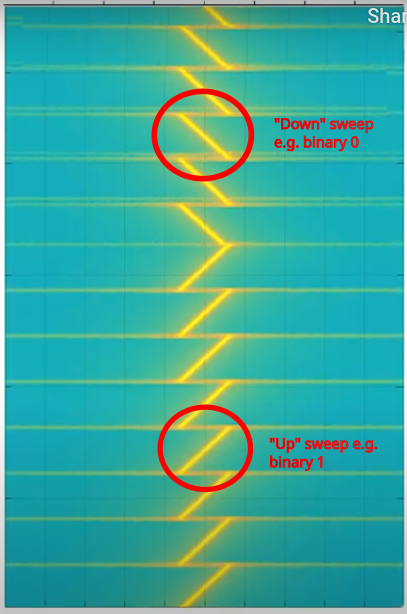
\includegraphics[width=0.5\textwidth]{images/chirp_spread_spectrum_labeled}
\caption{Example of a chirp spread spectrum transmission, highlighting the up and down sweeps which represent binary 1 and 0. \cite{Wenner2017_hd}}
\label{fig:chirp_spread_spectrum_labeled}
\end{figure}

Figure \ref{fig:chirp_spread_spectrum_labeled} provides a visual representation of the chirp spread spectrum technology. This technique encodes data in the frequency variation of the signals over time. A "chirp" refers to a timeframe of the signal where the frequency is increasing or decreasing within a certain bandwidth. This technique makes the signal significantly more resistant to interference compared to simply having two distinct frequencies which are pre-defined to represent a binary 0 or 1, and simply switching between them when transmitting the signal, an example of which can be seen in figure \ref{fig:frequency_shift_keying_labeled}. The up and down sweeps in figure \ref{fig:chirp_spread_spectrum_labeled} visually reflect the bitstream and how it is encoded into radio frequencies.

\begin{figure}[H]
\centering
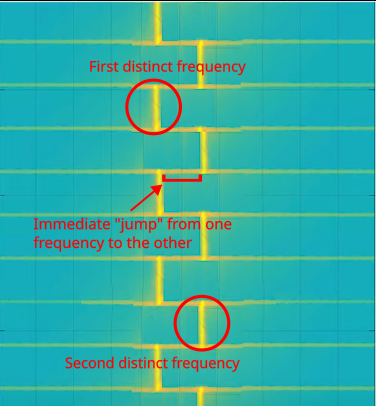
\includegraphics[width=0.5\textwidth]{images/frequency_shift_keying_labeled.png}
\caption{Example of having two distinct frequencies representing binary 0 and 1, and "jumping" between them instead of sweeping. \cite{Wenner2017_hd}}
\label{fig:frequency_shift_keying_labeled}
\end{figure}

Each character transmitted with LoRa lasts a duration determined by the spreading factor, defining how long each chirp lasts. As spreading factor increases, chirps last longer and have improved sensitivity at the expense of having a lower data transmission rate.

LoRaWAN builds upon the LoRa physical layer by adding a media access control (MAC) protocol. It defines how devices connect, how data is encrypted, and how the network is managed. LoRaWAN is designed for ultra-low-power operations, allowing devices to last several years on small batteries, and offers deep indoor penetration, which is particularly valuable in hospital settings where walls and medical equipment can attenuate signals \cite{lora_documentation}.

To assess the suitability of LoRaWAN, it is important to compare it to other LPWAN technologies, including SigFox, NB-IoT, and LTE-M.

SigFox is a proprietary ultra-narrowband communication technology designed for transmitting small data payloads over long distances, while consuming small amounts of power. It operates on unlicensed Industrial, Scientific, and Medical (ISM) bands, and works best when the application requries one-way, infrequent transmissions. These attributes make it great for low-throughput applications, such as smart city metering, and environmental monitoring. Due to some issues with non-fixed environments such as frequency inaccuracies and interference, SigFox works best when employed in fixed locations \cite{sigfox_advantages_disadvantages}.

NB-IoT on the other hand operates in the licensed spectrum. Developed by 3GPP, it offers powerful indoor penetration, is reliable, and allows for connecting a large number of devices. It is mainly suited for applications needing regular (unlike SigFox), low data rate communication, like utility metering and building automation \cite{nbiot_advantages_disadvantages}.

Once again developed by 3GPP, LTE-M supports higher data rates than NB-IoT and allows for voice communication using Voice over Long-Term Evolution (VoLTE). It ensures seamless handover between cell towers, which makes its use cases more dynamic and mobile, such as asset tracking, pet tracking, and point-of-sale devices \cite{ltem_telenor}.

Below is a table summarising their main advantages and disadvantages.

\begin{table}[H]
\centering
\caption{LPWAN technologies - Advantages \& Disadvantages \cite{sigfox_advantages_disadvantages, nbiot_advantages_disadvantages, ltem_advantages_disadvantages, lorawan_advantages_disadvantages}}
\begin{tabularx}{\textwidth}{l X X}
\toprule
\textbf{Technology} & \textbf{Advantages} & \textbf{Disadvantages} \\
\midrule
LoRaWAN &
\begin{itemize}
	\item Long range
	\item Low power consumption
	\item Adaptive data rates
	\item Deep indoor penetration
	\item Low cost
\end{itemize}
&
\begin{itemize}
	\item Limited by duty cycle
	\item Unsuitable for real-time or low latency applications
\end{itemize}
\\
SigFox &
\begin{itemize}
	\item Lightweight protocol
	\item Minimal overhead
	\item Long battery life
	\item Wide coverage
	\item Underground support
\end{itemize}
&
\begin{itemize}
	\item One-way communication
	\item Limited data rates
	\item One operator per country
\end{itemize}
\\
NB-IoT &
\begin{itemize}
	\item High scalability
	\item Robust QoS
	\item Extended range
	\item Structure penetration
	\item Backed by operators
\end{itemize}
&
\begin{itemize}
	\item Licensed spectrum costs
	\item Lower data rates than LTE-M
	\item No roaming support
\end{itemize}
\\
LTE-M &
\begin{itemize}
	\item High data rates
	\item Excellent coverage
	\item LTE network integration
	\item Efficient power use
\end{itemize}
&
\begin{itemize}
	\item Higher costs
	\item Firmware updates consume power
	\item Not for high-volume data
\end{itemize}
\\
\bottomrule
\end{tabularx}
\label{tab:lpwan_adv_disadv}
\end{table}



Bluetooth is also widely used in medical IoT devices. While it offers short-range connectivity and is well-suited for personal health devices like heart rate monitors and themometers, its power consumption and range limit its usefulness for hospital-wide or remote patient monitoring. Bluetooth Low Energy (BLE) improves power efficiency and is increasingly integrated into wearable medical devices. As such, it will be used in this project to connect the main system with the medical sensors which take actual readings.

\subsubsection{Testing}
While the focus of this project was not to benchmark the LoRaWAN protocol itself, preliminary simulations were conducted to validate its suitability for post-operative monitoring applications. A single base station scenario was simulated using open-source software provided by Lancaster University \cite{lancaster_uk_simulation_software}. The simulation was adapted to run on Python 3, and tests were conducted with 100 to 1000 node configurations, increasing by 100 each experiment. The parameters for the simulations where fixed as such: \texttt{AVGSEND = 100ms}, \texttt{SIMTIME = 2000ms}, and \texttt{COLLISION = 1} to enable full collision detection. The parameters used correspond to the simulated nodes transmitting small packets roughly every 100 milliseconds over a total simulation time of two seconds. Furthermore, \texttt{EXPERIMENT = 0} was used, which configures all nodes to transmit with the slowest LoRa modulation settings. The key objective was to confirm that LoRaWAN could handle multiple nodes transmitting small amounts of data at low power over long distances.

\vspace{1em} \noindent The first set of results explore how node density affects transmission quality:
\begin{figure}[H]
\centering
\begin{subfigure}{0.48\textwidth}
	\centering
	\begin{tikzpicture}
\begin{axis}[
	width=\textwidth,
	height=6cm,
	grid=both,
	xlabel={Number of Nodes},
	ylabel={Number of Collisions},
	title={Collisions vs Number of Nodes},
	tick label style={font=\small},
	label style={font=\small},
	title style={font=\small}
]
\addplot[
	color=orange,
	mark=*,
	thick
] table [x=Nodes, y=Collisions, col sep=comma] {graphs/collisions_vs_nodes_all.csv};
\end{axis}
\end{tikzpicture}

	\caption{Collisions vs Number of Nodes}
	\label{fig:collisions_vs_nodes}
\end{subfigure}
\hfill
\begin{subfigure}{0.48\textwidth}
	\centering
	\begin{tikzpicture}
\begin{axis}[
	width=\textwidth,
	height=6cm,
	grid=both,
	xlabel={Number of Nodes},
	ylabel={Transmissions per Node},
	title={Transmission Efficiency vs Number of Nodes},
	tick label style={font=\small},
	label style={font=\small},
	title style={font=\small}
]
\addplot[
	only marks,
	color=teal,
	mark=*,
	% thick
	mark options={scale=1}
] table [x=Nodes, y=Efficiency, col sep=comma] {graphs/efficiency_vs_nodes_all.csv};
\end{axis}
\end{tikzpicture}

	\caption{transmission Efficiency per Node}
	\label{fig:efficiency_vs_nodes}
\end{subfigure}
\caption{Impact of node count on number of collisions and transmission efficiency.}
\end{figure}

As per Figure \ref{fig:collisions_vs_nodes} the number of collisions increases with the number of nodes linearly, something that is consistent with LoRaWAN's unslotted ALOHA-based access scheme. Regardless, transmission efficiency (Figure \ref{fig:efficiency_vs_nodes}) remained relatively stable, even if it did drop slightly around the 500 node point. This demonstrates LoRaWAN's robustness even under increased load.

\vspace{1em} \noindent The next two plots look at power efficiency against the number of nodes, and the physical spatial distribution of the simulated nodes.

\begin{figure}[H]
\centering
\begin{subfigure}{0.48\textwidth}
	\centering
	\begin{tikzpicture}
\begin{axis}[
	width=\textwidth,
	height=6cm,
	grid=both,
	xlabel={Number of Nodes},
	ylabel={Energy Consumption},
	title={Energy Consumption vs Number of Nodes},
	tick label style={font=\small},
	label style={font=\small},
	title style={font=\small}
]
\addplot[
	color=purple,
	mark=*,
	thick
] table [x=Nodes, y=Energy, col sep=comma] {graphs/energy_vs_nodes_all.csv};
\end{axis}
\end{tikzpicture}

	\caption{Energy Consumption vs Number of Nodes}
	\label{fig:energy_vs_nodes}
\end{subfigure}
\hfill
\begin{subfigure}{0.48\textwidth}
	\centering
	\begin{tikzpicture}
\begin{axis}[
	width=\textwidth,
	height=6cm,
	grid=both,
	xlabel={X Coordinate},
	ylabel={Y Coordinate},
	title={Spatial Distribution of Nodes},
	axis equal
]
\addplot[
	only marks,
	mark=*,
	color=red,
	mark size=1pt
] table [x=X, y=Y, col sep=comma] {graphs/spatial_distribution_all.csv};
\end{axis}
\end{tikzpicture}

	\caption{Spatial Distribution of Nodes}
	\label{fig:spatial_distribution}
\end{subfigure}
\caption{Energy scalability and simulation topology.}
\end{figure}

Figure \ref{fig:energy_vs_nodes} shows that energy consumption of each node scaled linearly once more with the number of nodes. This is to be expected as all nodes use the same transmit settings and a fixed sending interval. Provided duty cycles are properly managed, these results support LoRaWAN's use in battery-powered applications. A duty cycle is the time a device is permitted to transmit on a given frequency band, within a set time period \cite{duty_cycles}. The spatial distribution (Figure \ref{fig:spatial_distribution}) simply confirms that the simulation used a random deployment of the nodes across the simulated physical area, approximating a real-world environment such as a hospital ward.

\vspace{1em} \noindent Path loss and signal strength trends were also considered to better understand signal behaviour.
\begin{figure}[H]
\centering
\begin{subfigure}{0.48\textwidth}
	\centering
	\centering
\begin{tikzpicture}
\begin{axis}[
	width=\textwidth,
	height=6cm,
	grid=both,
	xlabel={Distance (m)},
	ylabel={RSSI (dBm)},
	title={RSSI vs Distance}
]
\addplot[
	only marks,
	mark=*,
	color=blue,
	mark size=1pt
] table [x=Distance, y=RSSI, col sep=comma] {graphs/rssi_vs_distance_all.csv};
\end{axis}
\end{tikzpicture}
\caption{RSSI values relative to distance from the gateway.}

	\caption{RSSI vs Distance}
	\label{fig:rssi_vs_distance}
\end{subfigure}
\hfill
\begin{subfigure}{0.48\textwidth}
	\centering
	\centering
\begin{tikzpicture}
\begin{axis}[
	width=\textwidth,
	height=6cm,
	grid=both,
	xlabel={Distance (m)},
	ylabel={Lpl (dB)},
	title={Lpl vs Distance},
	tick label style={font=\small},
	label style={font=\small},
	title style={font=\small},
]
\addplot[
	only marks,
	mark=*,
	color=green,
	mark size=1pt
] table [x=Distance, y=Lpl, col sep=comma] {graphs/lpl_vs_distance_all.csv};
\end{axis}
\end{tikzpicture}
	\caption{Path loss (Lpl) values relative to node distance from the gateway.}

	\caption{Path Loss (Lpl) vs Distance}
	\label{fig:lpl_vs_distance}
\end{subfigure}
\caption{Signal strength and path loss trends relative to node distance from the gateway}
\end{figure}

Both path loss and Received Signal Strength Index (RSSI) degrade as the distance increases, which is to be expected based on theoretical radio propagation models. RSSI is a represents the measurement of power level for a received radio signal. It is typically expressed in dBm, and as the values get more negative, it indicates a weaker signal.

Results showed that as the number of nodes doubled, the number of collisions also increased, which is consistent with LoRaWAN's access behaviour. In this context, a \textit{collision} refers to the event where multiple decvices transmit at the same time, on the same frequency, and with the same spreading factor, at overlapping times, leading to signal interference at the gateway. When collisions occur, the gateway will likely have trouble demodulating the incoming transmitted packets, causing data loss.

Despite the increase in collisions, transmission efficiency per node remained stable, and energy consumption scaled predictably with the node count --- highlighting LoRaWAN's suitability for applications requiring scalability, wide coverage, and energy efficiency, such as this project. Compared to Wi-Fi, LoRaWAN uses significantly less power and has a vastly longer communication range. Wi-Fi needs to have constant connectivity, and frequently send beacons out informing end devices of available access points and services \cite{wifi_beacons}. These two facts mean Wi-Fi consumes substantially more power than LoRaWAN making it unsuitable for battery operated devices intended for long-term use (in the order of years). Furthermore, Wi-Fi was designed for high-throughput applications in a limited range in indoor environments, unlike LoRaWAN which was designed for sparse, low data rate transmission covering large areas. As for GSM-based technologies like NB-IoT and LTE-M, while they do offer broader coverage and existing infrastructure backed and maintained by mobile providers, they come with significantly higher costs, greater power needs, and licensing requirements (meaning legally only mobile network operators can operate them, or a partnership with a mobile operator is requried), making them not as suitable for this application as LoRaWAN is. The comparison in Table \ref{tab:lpwan_adv_disadv} illustrates the advantages of LoRaWAN in terms of its efficient power consumption, cost, and flexibility in deployment and operation.

These outcomes support the choice of LoRaWAN as a communication backbone in the system, balancing scalability and energy efficiency in a medical monitoring context.

\section{Commercially available medical devices} % Section 2.5
Because Bluetooth technology combined with technologies allowing integration with the cloud allow for continuous, real-time monitoring of vital signs including heart rate, blood pressure, respiration rate, temperature, and oxygen saturation, they have completely changed postoperative treatment. Such devices enable smooth data transfer to medical professionals, enabling prompt interventions and individualised patient treatment. Numerous Bluetooth-enabled medical devices are available on the market, with differences in performance, compatibility, and data access transparency. Since it dictates how easily these devices may be integrated with other healthcare systems and apps such as the one discussed in this thesis, the level of Bluetooth openness is especially important. I will examine a number of commercially available devices that demonstrate these characteristics in the sections that follow, emphasising their features and clinical application considerations.

Numerous commercially available medical devices can be used in clinical settings and are made for the continuous monitoring of vital signs. Selected devices are summarised in the table below, with an emphasis on those that have been certified for clinical use by the US Food and Drug Administration (FDA) or that bear the CE mark in accordance with the EU Medical Device Regulation. It is important to keep in mind that FDA approval entails a more stringent examination procedure and is frequently thought of as a higher quality of clinical validation, even if the CE mark certifies regulatory conformity.

The table features the certification granted to the device, the measured vital signs, and its Bluetooth openness level. Each device listed is capable of measuring one or more of the following vital signs:

\begin{itemize}
			\item \textbf{HR:} Heart Rate
			\item \textbf{BP:} Blood Pressure (may be traditional or cuffless)
			\item \textbf{RR:} Respiratory Rate
			\item \textbf{SpO\textsubscript{\textbf{2}}:} Blood Oxygen Saturation
			\item \textbf{Temp:} Body Temperature
			\item \textbf{ECG:} Electrocardiogram
\end{itemize}

The term "Bluetooth openness" indicates how simple it is to access and incorporate data into customised solutions. Interoperability may be a constraint for customised IoT solutions because the majority of clinically certified devices function within proprietary ecosystems.

\begin{table}[H]
\centering
\caption{Medically Certified Bluetooth Capable Devices}
	\renewcommand{\arraystretch}{1.2}
	\begin{tabularx}{\textwidth}{|>{\RaggedRight\arraybackslash}X|>{\RaggedRight\arraybackslash}X|>{\RaggedRight\arraybackslash}X|>{\RaggedRight\arraybackslash}X|>{\RaggedRight\arraybackslash}X|}
	\hline
	\textbf{Device Name} & \textbf{Manufacturer} & \textbf{Certification} & \textbf{Vital Signs it Measures} & \textbf{Bluetooth Openness} \\
	\hline
	GE Portrait Mobile & GE HealthCare & FDA & HR, RR, SpO$_2$, Temp & Closed \\ 
	\hline
	Berry Multi-Parameter Monitor & Berry Medical & CE (MDR) & HR, BP, SpO$_2$, Temp, ECG & Semi-open \\
	\hline
		Contec CMS8000 & Contec Medical & CE (MDR) & HR, BP, SpO$_2$, Temp, RR, ECG & Closed \\
		\hline
		Biobeat Chest Patch & Biobeat & FDA, CE (MDR) & HR, BP (cuffless), SpO$_2$, RR, Temp & Closed \\
		\hline
		Caretaker4 & Caretaker Medical & CE (MDR) & BP, HR, RR, SpO$_2$ & Closed \\
		\hline
		Checkme Pro Vital Signs Monitor & Wellue (Viatom) & CE (MDR) & HR, BP, SpO$_2$, Temp, ECG & Semi-open \\
		\hline
		CardiacSense Watch & CardiacSense & CE (MDR) & HR, ECG, SpO$_2$, Temp & Closed \\
		\hline
		SIFVITAL-1.2 & SIFSOF & CE (MDR) & HR, BP, SpO$_2$, Temp, Glucose & Closed \\
		\hline
		CARER HC-03 6-in-1 Monitor & CARER Medical & CE (MDR) & HR, BP, SpO$_2$, Temp, Glucose, ECG & Closed \\
		\hline
		Lepu Vital Signs Monitor & Lepu Medical & CE (MDR) & HR, BP, SpO$_2$, Temp, ECG & Closed \\
		\hline
	\end{tabularx}
	\renewcommand{\arraystretch}{1.0}
\label{tab:lpwan_adv_disadv}
\end{table}



Even though a lot of devices fulfil the requirements for medical certification, as the table shows, they frequently lack open Bluetooth interfaces. When incorporating them into custom IoT systems, this poses a problem, which will be discussed in the next section along with suggestions for dealing with it.

\section{Integration with custom IoT systems} % Section 2.6
Because of the restricted or proprietary nature of their Bluetooth communication protocols, it is still very difficult to integrate commercially available vital signs monitors into custom Internet of Things (IoT) systems. As mentioned in the preceding section, the majority of devices offer little to no support for open data access, despite the fact that many of them are medically certified and give accurate physiological readings. Some, at most, provide semi-open APIs that are restricted to partner software or vendor-specific apps. This makes it more difficult to integrate seamlessly with specially designed systems that seek to independently gather, process, or send data. The impacts of these restrictions are examined in this section, along with possible interoperability tactics for medical IoT applications.

\subsubsection{Challenges and Implications}
Even though there are medically recognised vital sign measurement devices available, Bluetooth accessibility issues make it difficult to integrate them into custom IoT systems. The majority of medical equipment intended for professional usage rely on closed data ecosystems or proprietary Bluetooth protocols. The functionality is frequently confined to vendor-approved apps or limited APIs, preventing complete integration with customised microcontroller-based systems, even in situations where some Bluetooth access is offered.

This lack of openness presents a number of practical and technical difficulties. First, there are significant limitations on compatibility. Raw vital sign data cannot be directly accessed by custom systems that depend on local gateways or lightweight edge devices (like Arduino or ESP32) unless the device supports standard Bluetooth Generic Attribute Profile (GATT) profiles or offers a published Application Programming Interface (API). Consequently, the two main advantages of edge-based IoT architectures—real-time processing and on-device decision-making—become impracticable. Second, vendor lock-in develops into an extremely serious issue. System designers are left with no control over data flow, privacy policies, and long-term data preservation when device data is only available via the cloud platforms or mobile apps of the manufacturer, which almost certainly makes it more difficult to comply with data protection laws like GDPR or HIPAA in clinical or research settings where data sovereignty, repeatability, and traceability are crucial.

Furthermore, development time and integration complexity also rise. Reverse engineering, unapproved Software Development Kits (SDKs), or intricate workarounds are frequently required in order to retrieve useful data from these devices. These endeavours are laborious, prone to mistakes, and possibly fragile, as they can fail with firmware changes or violate license agreements.

These difficulties show how the requirements for adaptable, responsive IoT-based monitoring solutions differ from those of authorised commercial devices. To overcome these constraints while maintaining system dependability and regulatory compliance, potential workarounds and integration techniques are examined in the immediately following paragraphs.

\subsubsection{Possible Solutions}
Developers of custom IoT systems must think of alternate ways to enable integration while preserving clinical dependability and compliance, given the limitations imposed by proprietary Bluetooth implementations in medically approved vital sign monitors. While there isn't a single solution that works for all, there are a few workarounds that could enable significant interoperability despite the existing constraints.

\begin{enumerate}
	\item \textbf{Use of intermediate devices with vendor APIs}
	\item[] Data can be accessed by official desktop software or mobile applications in certain closed systems. In these situations, middleware bridges that communicate with the vendor software through open SDKs or REST APIs can be created, such as companion Raspberry Pi services or smartphone apps. These intermediary devices can then use standardised protocols to send the necessary information to customised IoT devices. This maintains data accuracy and honours the device's intended usage paradigm, even if it adds another layer of complexity and can cause latency to increase.
	\item \textbf{Preferring semi-open devices to entirely closed devices}
	\item[] Vendors occasionally offer limited Bluetooth access via documented GATT profiles or custom services. Although they are not completely open, devices like the Wellue Checkme Pro provide restricted data access that can be adequate for everyday uses. When feasible, system designers should give priority to these semi-open devices and use reverse-engineered documentation or community-developed libraries to retrieve readings with the least amount of intrusion to prevent any legal problems regarding licensing agreements.
	\item \textbf{Passive signal interception (may violate licensing agreements)}
	\item[] Certain specialised tools can be used to determine the transmission structure of the Bluetooth signals sent from closed sensor devices, and reverse-engineer the communication protocol in devices without access to an API or access point. Although this method can provide complete access to sensor data, it is not recommended for production systems or environments that need to adhere to legal or clinical requirements since it runs the risk of breaking user agreements and regulatory restrictions.
	\item \textbf{Develop sensor systems in parallel}
	\item[] By constructing parallel sensor modules with clinically proven open hardware or certified discrete sensors (e.g., MAX30101 for SpO$_2$ and pulse, MLX90614 for temperature), it is also possible to entirely eliminate reliance on closed devices. This provides complete firmware-level control over sensing, communication, and data handling, but it is more taxing in terms of development resources. Full-stack customisation is made possible by the direct integration of such customised sensors with system infrastructure when paired with LoRa, BLE, or Wi-Fi transmission modules.
	\item \textbf{Collaboration with vendors and enterprise partnerships}
	\item [] Organisations can contact vendors for OEM agreements or developer access when commercial devices are preferred. On request, certain manufacturers might provide enterprise SDKs or documentation, particularly for system integration pilot programs, academic research, or clinical trials. Even though it could take more time, this approach guarantees long-term support and compliance.
	\item[] The expense, complexity, and legality of each of these workarounds are trade-offs. The best strategy frequently calls for a hybrid system, in which open or semi-open alternatives are utilised for system development or simulation, while medically certified but closed devices are utilised for clinical validation. In the end, market forces and regulatory pressure may push manufacturers towards greater openness in upcoming device generations as the need for patient-specific, interoperable healthcare systems increases.
\end{enumerate}

\section{Summary} % Section 2.7
There are technological and legal issues with integrating medically approved vital sign monitoring devices into unique IoT systems. Even if a lot of commercial devices provide precise and trustworthy measurements, smooth integration is hampered by their closed or semi-open Bluetooth implementations, which restrict direct access to raw data streams. These restrictions may affect custom healthcare platforms' adaptability, reactivity, and independence. However, there are a number of practical alternatives, such as using semi-open devices, developing parallel sensing modules, using middleware programs, or forming direct relationships with manufacturers. For IoT healthcare solutions to be scalable, interoperable, and patient-tailored, these integration hurdles must be removed.


\chapter{Analysis and Design}

\section{Introduction} % Section 3.1
This chapter will present the analysis and design porition of the project. Identified are the system users and their needs, which are then translated into technical requirements, and finally the system's functional and architectural design is described. Several diagrams are included to aid with visualising the behaviour, workflow, and structure of the system.

\section{User Needs and Requirements} % Section 3.2
When developing any technology it is imperative to have a solid foundation upon which to build on and refer to throughout the development process. It should help provide a clear understanding of the problem, the needs and expectations of the people who will be using it, and give some insight into how the original problem will be solved in the implementation stage. In the case of this project, the users include nurses and doctors, and the patients who will be using the device. There are several different users each with different required levels of control and functionalities, therefore it is crucial to translate their needs into measurable and clearly defined requirements that will steer the design and eventually implementation of the system.

The following pages present two key tables accomplishing that task: the \textbf{User Needs table} (Table \ref{tab:user_needs_table}), and the \textbf{User Requirements table} (Table \ref{tab:user_requirements_table}). The User Needs table outlines what the system should accomplish in simple terms, similar to how an average non-technical person might describe what they need to solve their problem. Each row consists of a unique \textbf{ID} for that particular need, a brief \textbf{Description} of what is needed, and a \textbf{Source} which represents what part of the system this need might be addressed in. The User Requirements table expands upon the User Needs table by translating each need into one or more clear and actionable system requirements. These requirements can be measured as satisfied or not in the final system. Each requirement has a unique \textbf{Req. ID}, a \textbf{User Requirement Name} giving a very short overview of what that requirement is supposed to do, and a \textbf{Description} of the requirement with more specific technical details such as how it might be implemented, what specific numeric constraints are present for it, or what exactly is required to satisfy it from a technical perspective. Following these are the \textbf{Justification/Comment} and the \textbf{Reference} columns. The Justification/Comment column expands a bit on the description and states \textit{why} some of the technical details are as they are, or why the requirement was necessary in the first place. The Reference column links the User Requirements Table to the User Needs table by stating what user need (or what multiple needs) a particular requirement is intended to satisfy.

These tables together give a high-level perspective of what the system must achieve, with some justification as to why certain decisions where taken instead of others.

\begin{landscape}
\thispagestyle{empty}
\begin{table}[H]
\centering
\caption{User Needs Table}
% \begin{tabularx}{\linewidth}{|p{2.5cm}|p{15cm}|p{1.5cm}|}
\begin{tabularx}{\linewidth}{|p{2.5cm}|X|p{2cm}|}
\hline 
\textbf{ID} & \textbf{Description } & \textbf{Source} \\
\hline
UN-01 & Accurate capture of data from various medical devices in order to monitor patient status & Arduino \\
\hline
UN-02 & Simple pairing of the device to other medical devices through Bluetooth in order to easily setup and guarantee reliable data transfer & Arduino \\
\hline
UN-03 & Updating/setting of limits/conditions for different measurement types in order to customise each device to a particular patient's needs & Arduino/\newline Cloud/\newline Medical staff \\
\hline
UN-04 & Process data according to preset conditions in order to send only relevant data to the cloud & Arduino \\
\hline
UN-05 & Storing of data in the short-term in the case of high network congestion to prevent loss. (Only store after processing if values are abnormal/relevant to be sent to the cloud) & Arduino \\
\hline
UN-06 & Alert medical staff of patient status if critical or abnormal reading gathered in order to allow them to check on said patient in person & Cloud \\
\hline
UN-07 & Alert users about device status in order to allow them to keep it in a state where it is running normally & Arduino \\
\hline
UN-08 & Provide a general picture about the patient's status daily in order to track it over time (daily averages viewed in context of weeks, months, years) & Cloud \\
\hline
\end{tabularx}
\label{tab:user_needs_table}
\end{table}
\end{landscape}

\clearpage
\pagestyle{empty}
\begin{landscape}
% \begin{table}[H]
% \centering
\begin{longtable}{|p{2cm}|>{\RaggedRight\arraybackslash}p{6cm}|>{\RaggedRight\arraybackslash}p{6cm}|>{\RaggedRight\arraybackslash}p{6cm}|p{2cm}|}
\caption{User Needs Table}
\label{tab:user_requirements_table} \\
\hline 
\textbf{Req. ID} & \textbf{User Requirement Name} & \textbf{Description} & \textbf{Justification/Comment} & \textbf{Reference}\\
\hline
\endfirsthead

\hline
\textbf{Req. ID} & \textbf{User Requirement Name} & \textbf{Description} & \textbf{Justification/Comment} & \textbf{Reference}\\
\hline
\endhead

\hline
\endfoot

\hline
\endlastfoot

UR-01 & Temperature Reading & 5 times/12 hours\newline Accuracy: to nearest 0.1$^\circ$C & 5 readings in a single 12 hour period should be enough to detect any changes in temperature early enough after they get out of bounds & UN-01 \\
\hline
UR-02 & Blood Pressure Reading & 1 time/12 hours\newline Accuracy: $\pm$3mmHg for both systolic and diastolic & The recommended number of times to measure BP is once per day & UN-01 \\
\hline
UR-03 & Heart Rate Reading & 3 readings spaced 2 minutes apart / hour, and keeping the average of the 3 readings as final BPM value\newline Accuracy: $\pm$ 5 BPM & In a clinical/hospital environment there would be constant EKG measurement so there is no reason medically not to measure heart rate as often as possible. However to conserve battery, avoid network congestion, and keep the processor constantly working, 3 readings averaged on the hour is sufficient for this system & UN-01 \\
\hline
UR-04 & Bluetooth Pairing with Medical Devices & Visual interface to display BT connection status, and allow force disconnecting a device which has connected if it is not a medical device & Pairing with a device should be incredibly easy seeing as a likely user group will be elderly individuals & UN-02 \\
\hline
UR-05 & Per Vital Sign Configuration & Visual interface to be able to select a vital sign that will be measured, and set the upper and lower acceptable limits for it. This must persist across power loss and general restarting of the device. In addition, the limits must make sense in the context of the vital sign they relate to. For example it should be impossible to set an upper limit of 60$^\circ$C for temperature & Each patient has different medical needs and as such will need customised ranges for the acceptable readings. Furthermore, the patients should not be required to have to set these limits in the event of a power loss of the device or device restart & UN-03 \\
\hline
UR-06 & Data Processing and sending to the cloud & Process each data reading in the context of the device type's pre-set limits (lower/upper). Readings which are below/above the limits will be added to a queue. The front data will be sent to the cloud using the LoRaWAN protocol. Once confirmation is received that the data is successfully received, it will be dequeued and the next data (if it exists) will be transmitted. Allow up to 3 attempts before considering that there is a problem with the device/connection to the network and alerting the user. & Data that is within the acceptable limits does not need to be sent. The queue's purpose is to ensure any critical readings get to the cloud platform where the medical professionals can respond accordingly. & UN-04 \newline UN-05 \\
\hline
UR-07 & Notification of medical staff for abnormal reading & After sending data through the LoRaWAN protocol to the cloud, create some kind of notification for the medical staff in the form of of an email or "ticketing" system & A popup notification is not sufficient because it might be missed & UN-05 \newline UN-06 \\
\hline
UR-08 & Device status information & Constantly monitor device status (BT connection, state) and display this information to the user & Due to the fact that status information must always be visible, and we do not want to occupy the LCD screen with it all the time, the information will be available through coloured LED lights & UN-07 \\
\hline
UR-09 & Patient status tracking over time & Regardless of whether an abnormal reading is gathered, at fixed times of the day and for a set number of times, take readings and send them to the cloud even if they are not abnormal. & Patient history could be vital for providing medical staff with insight into the patient's condition, however there is no need to take more than one non-abnormal reading per day & UN-08 \\
\hline
\end{longtable}
% \end{table}
\end{landscape}

\clearpage

\section{Use Cases and System Interactions} % Section 3.3
The Vital Sign Monitoring System allows for on-demand monitoring of key physiological parameters in postoperative patients, enabling prompt medical intervention and remote supervision. Medical personnel like doctors and nurses, as well as patients are the intended users of the system, and they engage with the it in several ways.

\subsection{Medical Staff Use Cases}
\begin{itemize}
	\item \textbf{Set Vital Sign Thresholds Remotely}
	\item[] Each patient's vital signs have upper and lower limitations that can be set by medical personnel remotely. By using these thresholds, out-of-bounds readings are automatically flagged and sent to the cloud platform.
	\item \textbf{Send Alert to Take Reading}
	\item[] The system can be manually prompted by a physician or nurse to ask the patient for a new measurement.
	\item \textbf{View Readings on Cloud Platform}
	\item[] Medical staff can view current and past readings remotely, via a web dashboard.
	\item \textbf{Receive Notification if Patient Status Abnormal}
	\item[] The system notifies the clinician when a vital sign is below or above the predetermined threshold.
	\item \textbf{Take Reading from Medical Sensor Device}
	\item[] Medical staff can initiate a reading automatically from the cloud platform. If there is no medical sensor connected with Bluetooth at that time, it will switch to prompting the user to connect one and take the reading themselves.
\end{itemize}

\subsection{Patient Use Cases}
\begin{itemize}
	\item \textbf{Receive Alert to Take Reading}
	\item[] When a measurement is required, the patient is prompted (both visually through the LCD screen and the LEDs, and audibly through the buzzer) that a reading is requested and what vital sign they should measure.
	\item \textbf{Control Medical Sensor Device Bluetooth LE Connection Status}
	\item[] Can connect or disconnect vital sign sensors to the device through Bluetooth LE.
	\item \textbf{Take Reading from Medical Sensor Device}
	\item[] Patients can manually take readings at times of their choosing, and take readings when directed to remotely by medical staff.
\end{itemize}

\begin{figure}[H]
	\centering
	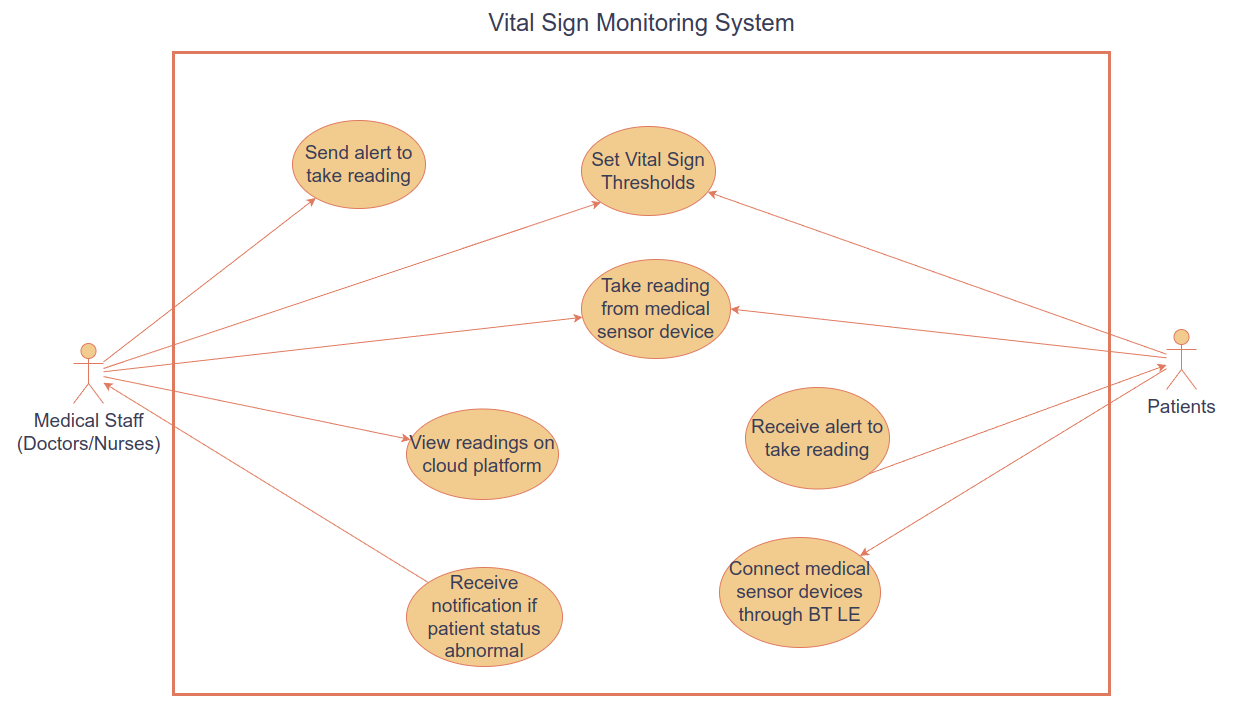
\includegraphics[width=\textwidth]{diagrams/use_case_diagram}
	\caption{Medical staff and patient interactions with the system}
	\label{fig:use_case_diagram}
\end{figure}

Following these exchanges, the system behaviour depicted in Figure \ref{fig:use_case_diagram} shows how the two user categories and the underlying monitoring functions are related. Every user role has a different workflow, as the diagram illustrates. Notably, the system will ask the patient to connect a compatible device and take the reading manually if medical staff requests a reading but there isn't a Bluetooth-connected medical sensor available at the moment. However, the use case diagram does not depict this internal fallback behaviour because these diagrams are meant to depict the actions that each actor can take that are visible to the outside world, not the internal logic or decision flows of the system. Nonetheless, this system ensures that clinical workflows are robust even when there are disconnections and that monitoring capability is maintained.

In conclusion, the system outlines the responsibilities of both patients and medical staff clearly, and takes into account situations where a reading is requested but there is no device connected to take it. Patients can also take readings throughout the day if they so desire, but when there is a remote request from a clinician it can not be ignored.

The system architecture and behavioural design, including state diagrams and the circuit diagram, are shown in the next section.

\section{System Architecture and Design} % Section 3.4
The architecture and design of the system are described in this section. For long-distance, low-power data transmission and centralised monitoring, the system includes a microcontroller-based LoRa communication unit. To gather data from the vital sign sensors, a Bluetooth Low Energy module is used, and for the communication between the device and the cloud a LoRaWAN gateway is set up to transmit to TheThingsNetwork. The goal of the design is to make it capable of communicating with BLE devices as simply as possible (something that due to the current closed nature of commerically available medical BT devices is not as simple as would be ideal), while utilising LoRaWAN's low-power features to allow for scalable, remote vital sign collecting, which is perfect for post-operative settings or locations with inadequate infrastructure.

Three main phases make up the system design: data collection (using the Bluetooth module to collect readings from medical sensors), processing of said data and finally transmission using an Arduino-based LoRa node. To tie everything together, cloud integration (using a LoRaWAN gateway and backend) will consist of a simple platform to view data and send commands to the device from a regular browser.

A high-level overview of the system's design is shown in Figure \ref{fig:high_level_architecture_diagram}. Blood pressure sensors, temperature sensors, and heart rate sensors are examples of medical Bluetooth capable devices that connect to a central unit (an Arduino-based microcontroller with a LoRa module) via Bluetooth LE. This central unit acts as a command centre and filter at the same time, where it filters out read data and only sends that which exceeds the set thresholds and is therefore considered critical data for a particular patient. It ignores data within bounds in all but a few cases --- those being when medical staff specifically request a reading, or the reading is one of those that are to be taken at set times every day.

This clearly compartmentalised architecture allows for separation of responsibilities: sensor management and handling of data is done locally, while the data is stored and analysed on the cloud platform. The cloud platform is also responsible for sending commands to the device when required by the medical staff.

\begin{figure}[H]
\centering
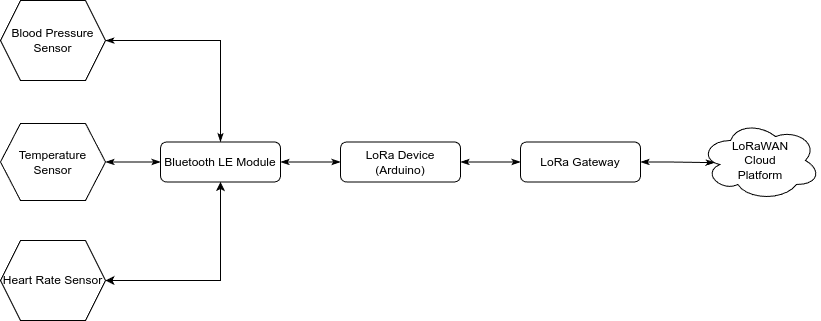
\includegraphics[width=\textwidth]{diagrams/high_level_architecture}
\caption{A high level view of the system architecture}
\label{fig:high_level_architecture_diagram}
\end{figure}

On the right side of Figure \ref{fig:high_level_architecture_diagram} is the LoRa Gateway which is responsible for bridging the device and the cloud platform.

The internal architecture of the embedded system is depicted in Figure \ref{fig:block_diagram}, which also highlights the hardware components' interactions on the Arduino-based microcontroller. The particular modules utilised in the finished implementation are shown in this diagram along with their functions in data collection, user interaction, processing, and communication.

\begin{figure}[H]
\centering
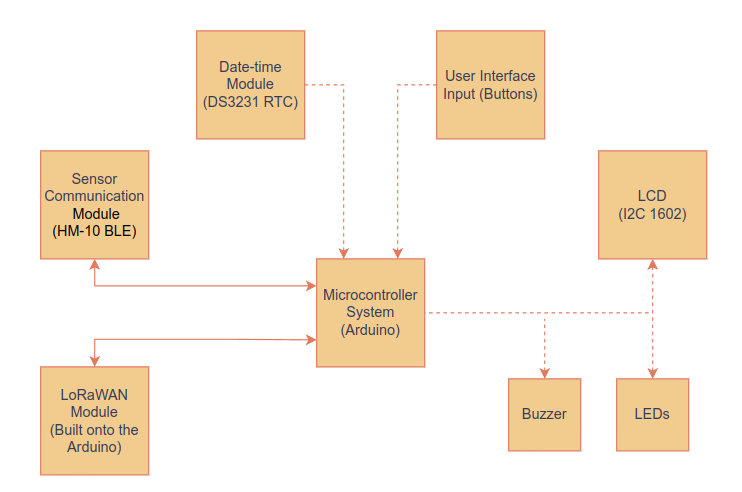
\includegraphics[width=\textwidth]{diagrams/block_diagram}
\caption{Block diagram showing relationships between high-level components of the system}
\label{fig:block_diagram}
\end{figure}

The core of the system is the Arduino microcontroller, which controls all data flow and peripheral interactions.

\begin{itemize}
	\item[] \textbf{Components for Sensing and Input}
	\item Module for Sensor Communication (HM-10 BLE): Communication with external medical devices, such as temperature, heart rate, and blood pressure sensors, is managed by this Bluetooth Low Energy module. This module is used by the Arduino to read data from the paired sensors.
	\item Date-Time Module: Accurate timestamps for sensor readings and intitiation of data reading at pre-programmed times of the day is provided by a real-time clock module (DS3231 RTC). This is crucial for monitoring vital sign trends over time. This data is read by the Arduino through I$^2$C.
	\item User Interface Input (Buttons): The patient can initiate actions, including entering reading mode and waiting for a reading or exploring menus on the display, by pressing buttons. This provides simple interaction without the need for additional devices.
	\item[] \textbf{Output and Feedback} 
	\item LCD Display: Shows timestamps, sensor data, and UI prompts in real time. This display uses very little GPIO thanks to the I$^2$C protocol.
	\item Local alarms are provided by the buzzer and the LEDs. System states, such as connected or disconnected, reading, processing, or errors can be represented by LEDs, and in the event of unusual readings or the need for user action, their attention can be grabbed by the use of the buzzer.
	\item[] \textbf{Transmission and Communication}
	\item LoRaWAN Module: This module manages wireless data transfer over great distances and is integrated into the Arduino board. After being taken and formatted, a reading is sent to the gateway via LoRa and uploaded to the cloud.
\end{itemize}

The system's behaviour can be varied based on the context and connected sensor thanks to its modular design using a Finite State Machine. Additionally, separated troubleshooting, streamlined development, and simpler future extensions (such incorporating SpO$_2$ sensors or supporting more sophisticated interfaces) are made possible by the separation of the communication, interface, and alarm modules. Next we will discuss the FSM that allows for this modularisation.

\subsubsection{State Machine Diagrams}
As soon as the system is turned on, it goes into the DISCONNECTED state. Awaiting user or environmental input, this state acts as the initial idle condition. In this state, two main conditions are assessed:

\begin{itemize}
	\item Without additional user interaction, the system switches straight to the CONNECTED state whenever a Bluetooth connection is discovered. When a compatible medical sensor is already activated and within range, this guarantees a smooth interaction.
	\item As an alternative, the system enters the SETUP state when the user chooses the "Setup" option from the interface, enabling the setting of vital sign thresholds before any sensors are connected.
\end{itemize}

\begin{figure}[H]
	\centering
	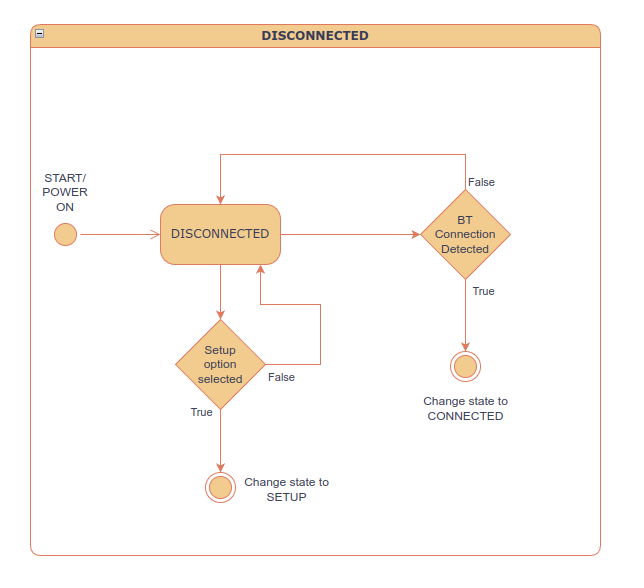
\includegraphics[width=\textwidth]{diagrams/states_disconnected}
	\caption{State diagram for the DISCONNECTED state}
	\label{fig:states_disconnected}
\end{figure}

Whether waiting for an automatic connection or permitting pre-configuration prior to active use, the decision structure guarantees flexibility and user-friendliness in the beginning stages of powering on (not requiring the user to explicitly enter the CONNECTED state if a device is already connected). The system can go on to measurement and data handling capability after configuration is finished or a device connects.

This flow can be seen visually represented as a state diagram in Figure \ref{fig:states_disconnected} above.

After a successful Bluetooth Low Energy (BLE) connection has been made with a medical sensor device, the CONNECTED state serves as the system's primary operating mode. In this condition, the user can take measurements or set up system parameters and has complete access to the system's essential features.

\begin{figure}[H]
	\centering
	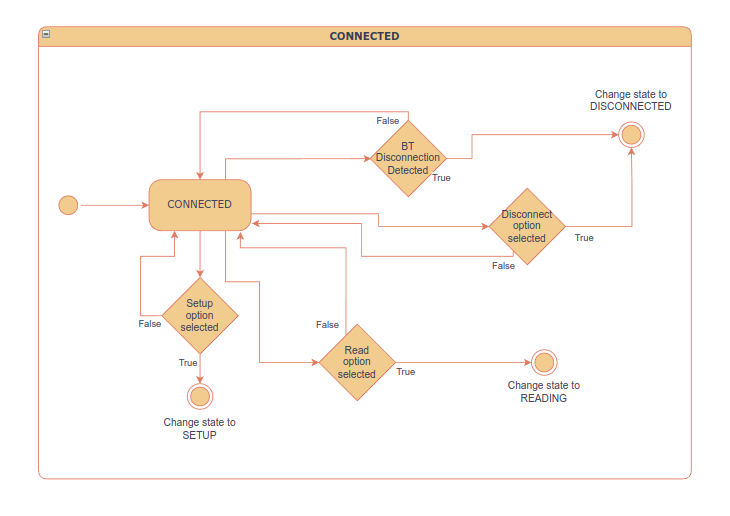
\includegraphics[width=\textwidth]{diagrams/states_connected}
	\caption{State diagram for the CONNECTED state}
	\label{fig:states_connected}
\end{figure}

The system offers three options from this state:

\begin{itemize}
	\item Setup: If the user selects the Setup option, the system enters the SETUP state, enabling the setup of vital sign thresholds.
	\item Read: Choosing the Read option puts the device in the READING mode and starts the process of gathering vital sign information from the linked medical sensor.
	\item Disconnect: The system returns to the DISCONNECTED state if the Disconnect option is chosen or if a Bluetooth disconnection is automatically detected. This guarantees that the availability of a linked sensor is always appropriately reflected by the system.
\end{itemize}

By ensuring that the system responds to user input as well as environmental changes (such a loss of connectivity), the state diagram preserves the system's resilience and user friendliness. Thus, the CONNECTED state acts as the centre for processes related to both configuration and data collection.

The interface for configuring the system's vital sign thresholds is accessible during the SETUP state. Depending on whether a Bluetooth-enabled sensor is currently coupled with the system, one can enter this state from either the DISCONNECTED or CONNECTED states.

\begin{figure}[H]
	\centering
	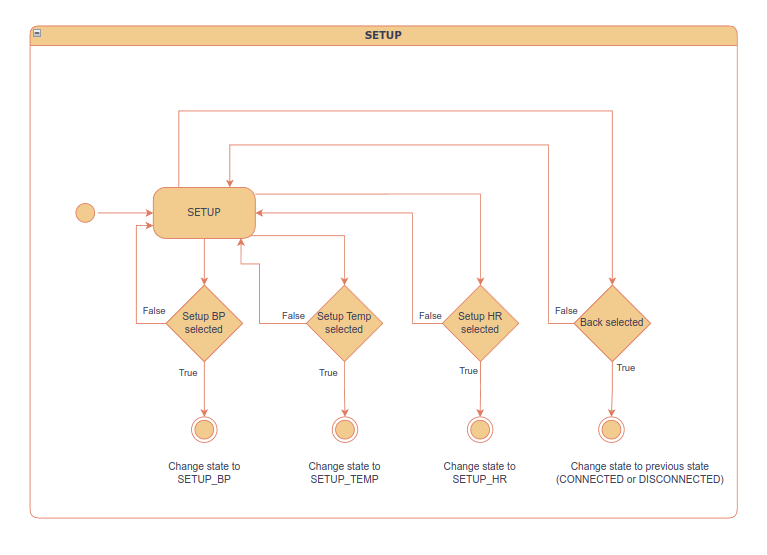
\includegraphics[width=\textwidth]{diagrams/states_setup}
	\caption{State diagram for the SETUP state}
	\label{fig:states_setup}
\end{figure}

As is visible from Figure \ref{fig:states_setup}, after entering the SETUP state, the user is given four options:

\begin{itemize}
	\item Setup BP (blood Pressure): This leads to the SETUP\_BP state, where the user can set the minimum and maximum systolic and diastolic thresholds accordingly.
	\item Setup Temp (Temperature): Allows the user to set the minimum and maximum temperature values by leading to the SETUP\_TEMP state.
	\item Setup HR (Heart Rate): This leads to the SETUP\_HR state where the user can set the minimum and maximum values for heart rate.
	\item Depending on where the SETUP state was called from, selecting the "Back" option will return the user to the CONNECTED or DISCONNECTED accordingly.
\end{itemize}

By serving as a routing hub, this state makes it possible to set clinical thresholds for each patient or surgery type. Each configuration option leads to a specific sub-state that handles validation and data entry logic; no threshold adjustments are made within this state itself.

The diagram below (Figure \ref{fig:states_setup_substates}) goes into detail for each of the setup sub-states.

\begin{figure}[H]
	\centering
	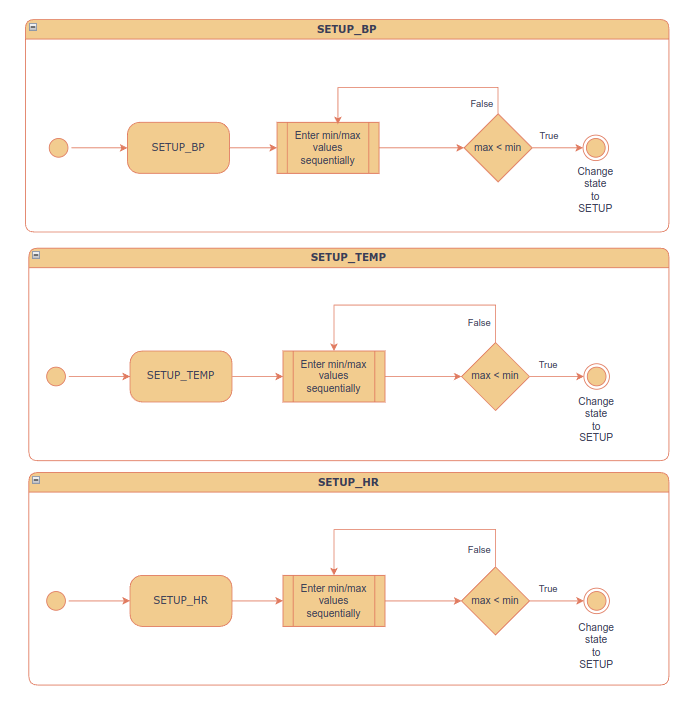
\includegraphics[width=\textwidth]{diagrams/states_setup_substates}
	\caption{State diagram for the SETUP sub-states}
	\label{fig:states_setup_substates}
\end{figure}

SETUP\_BP, SETUP\_TEMP, and SETUP\_HR are specifically responsible for setting the lowest and highest acceptable values for a given vital sign. The user is prompted to enter the values one after the other. To make sure the minimum is less than or equal to the maximum, each pair is separately checked. The system will re-prompt for both values if any validation is unsuccessful.

\begin{itemize}
	\item All of these states are essentially identical in structure and operation. They ask the user to enter a minimum and maximum value, check that the maximum is not less than the minimum, and if it is not return the user to the SETUP state.
\end{itemize}

These sub-states guarantee that threshold values used for measurement and analysis are reasonable, and enforce that thresholds are correctly set.

The READING state (Figure \ref{fig:states_reading}) is in charge of receiving vital sign information from a connected Bluetooth medical sensor. The system will wait for incoming data from the sensor device until something is received.

\begin{figure}[H]
	\centering
	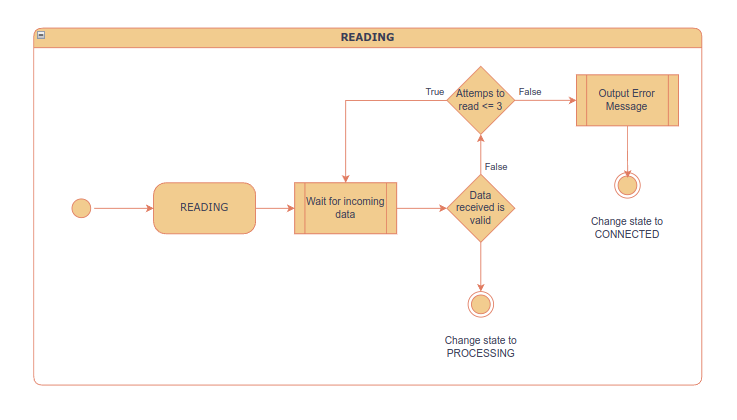
\includegraphics[width=\textwidth]{diagrams/states_reading}
	\caption{State diagram for the READING state}
	\label{fig:states_reading}
\end{figure}

Following the receipt of data, it must confirm that it's valid:

\begin{itemize}
	\item The system moves on to the PROCESSING state for more analysis if valid data is received.
	\item The system counts the number of read attempts if the data received is deemed invalid. Up to three attempts to read valid data are allowed.
	\item The system rejects the data and waits for a new reading if the number of attempts is less than or equal to three.
	\item The user is presented with an error message and the system returns to the CONNECTED state if the third attempt is unsuccessful as well.
\end{itemize}

The vital sign reading obtained in the previous READING state must be assessed by the PROCESSING state (Figure \ref{fig:states_processing}). The system determines if the newly received data is within the established acceptable bounds after it has been received. These thresholds, which are unique to each type of vital sign (e.g., blood pressure, heart rate, temperature), are established by the medical team or patient during system setup.

\begin{figure}[H]
	\centering
	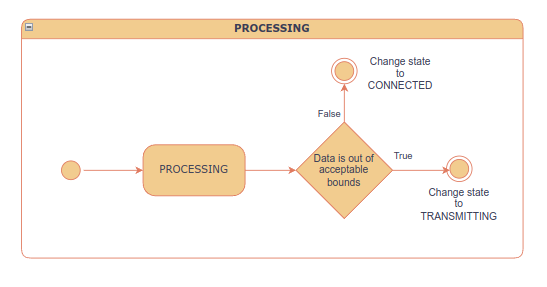
\includegraphics[width=\textwidth]{diagrams/states_processing}
	\caption{State diagram for the PROCESSING state}
	\label{fig:states_processing}
\end{figure}

The system returns to the CONNECTED state, where additional user input or new readings may be analysed, if the data falls within acceptable bounds and it decides that no immediate action is necessary. This is done to not flood the network with unnecessary traffic.

The data may, however, point to a potentially hazardous or abnormal patient condition if it drops below or goes above the established threshold range. The system then switches to the TRANSMITTING state, where it tries to transmit the abnormal reading to the cloud platform so that medical professionals can monitor it remotely.

This design ensures that alerts are raised only for clinically relevant events, reducing false alarms while maintaining responsiveness to potentially critical conditions, and reduces load on the network by only sending relevant data to the cloud.

Abnormal vital sign readings must be sent via LoRaWAN to the cloud platform while in the TRANSMITTING state (Figure \ref{fig:states_transmitting}). This only happens when a reading is outside the configured acceptable range, which indicates a possible health concern. This is determined by the PROCESSING state.

When the system reaches this state, the LoRa module on the Arduino starts the data transfer, after which it awaits confirmation from the cloud platform that the data was successfully received.

\begin{figure}[H]
	\centering
	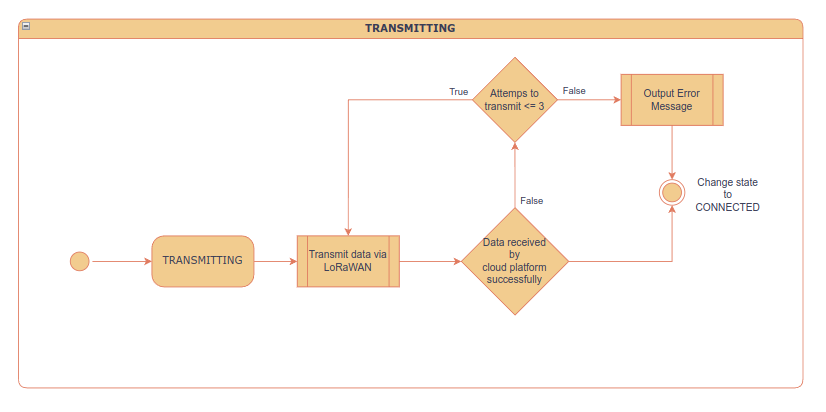
\includegraphics[width=\textwidth]{diagrams/states_transmitting}
	\caption{State diagram for the TRANSMITTING state}
	\label{fig:states_transmitting}
\end{figure}

Data transmission is deemed successful if confirmation is obtained in the form of an acknowledgement from the cloud platform, and the system goes back to the CONNECTED state, prepared to accept more inputs.

The system will attempt to deliver the data up to three times in the case of a failed transmission. The system notifies the user of the failure with an error message and returns to the CONNECTED state if, after three unsuccessful attempts, the data is still unable to reach the cloud platform. In addition to keeping the system from becoming permanently trapped in a failed state, this three-retries process helps guarantee reliability in wireless data transmission, particularly in settings where LoRaWAN connectivity may be erratic.

\subsubsection{Circuit Schematic}
The hardware circuit schematic for the system is displayed in Figure \ref{fig:circuit_diagram}. The system heart is the Arduino Leonardo microcontroller, which manages interfacing with peripheral components such the HM-10 Bluetooth Low Energy (BLE) module and the DS3231 real-time clock connected via I$^2$C. While the BLE module enables wireless connectivity to external sensor devices, the RTC maintains precise timekeeping for timestamping collected data, among other tasks.
The three-button interface allows for very basic user interaction in the form of menu navigation and threshold value entry. Four status LEDs—green, yellow, red, and blue—show the device's condition and Bluetooth connectivity. Additionally, a buzzer provides audible alerts for abnormal readings or transmission failures, and a 16x2 LCD display (as with the RTC, also connected via I$^2$C) is used to display menus. To guarantee a clear digital signal, a pull-down resistor is attached to each button, and 220 ohm resistors are used to limit the current flowing through all of the LEDs. This schematic represents a small, power-efficient design.
\begin{figure}[H]
\centering
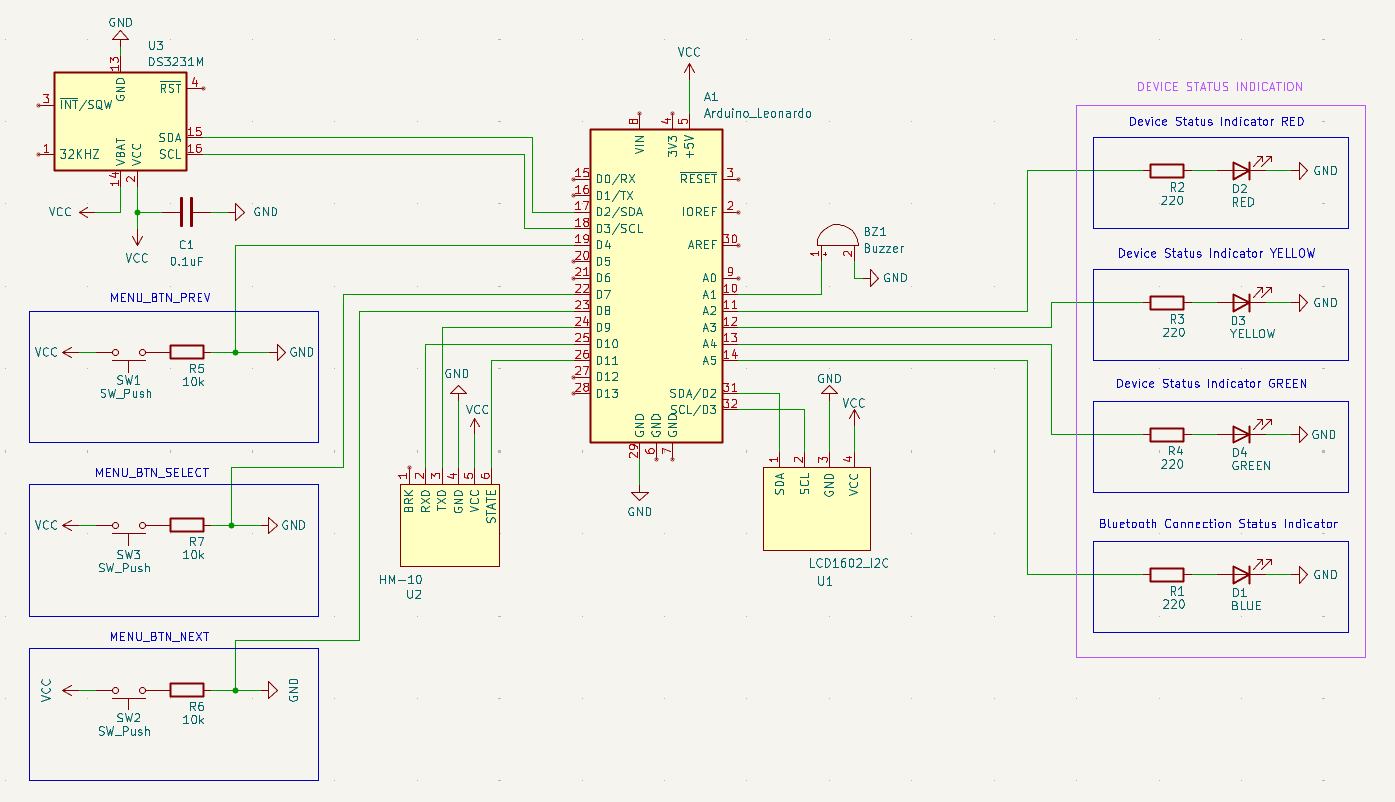
\includegraphics[width=\textwidth]{diagrams/schematic_rev3}
\caption{Detailed circuit shcemtatic of all all components in the device}
\label{fig:circuit_diagram}
\end{figure}

\section{User Interface Design} % Section 3.5
The device's user interface was made to be simple and easy to use, accommodating embedded technology limitations while guaranteeing medical staff and patients alike could easily interact with it. Push buttons, an LCD screen, a buzzer, and a group of LEDs make up the interface's four primary elements. Each one has a distinct function in communicating system status while occasionally their feedback cues may overlap to tell the user the same thing in different ways (e.g. Error displayed on the LCD while simultaneously a buzzer tone sounds corresponding to that error).

In addition to the device UI, there is the cloud dashboard UI, which I made using the TagoIO platform. It is split into four sections:
\begin{enumerate}
	\item \textbf{Commands:} This is where medical staff can send commands to the device such as a request for a reading or remote setting of vital sign thresholds (see Appendix~\ref{appendix:tagoio_commands}).
	\item \textbf{Blood Pressure:} This is where recevied blood pressure data can be visualised in two forms --- a vertical column view, and a line chart. (see Appendix~\ref{appendix:tagoio_bp})
	\item \textbf{Temperature:} This is where received temperature data can be visualised as a line chart. (see Appendix~\ref{appendix:tagoio_temp})
	\item \textbf{Heart Rate:} This is where received heart rate data can be visualised as a line chart. (see Appendix~\ref{appendix:tagoio_hr})
\end{enumerate}

Finally, I made a simple mobile app for testing purposes, to allow me to simply simulate medical sensors and their interactions with the system. The app's UI has four screens, with the main screen changing its appearance based on the connection status.
\begin{enumerate}
	\item \textbf{Main screen when first opening the app:} Contains an area to display simple logs, a button to clear the logs, and a button to start scanning for Bluetooth devices (see Appendix~\ref{appendix:app_ui_disconnected}).
	\item \textbf{Main screen when scanning for bluetooth devices:} When the button to start scanning is pressed, it changes to contain the text "Stop Scanning", and a list of available Bluetooth devices appears below it. When an item in the list is clicked, a connection is attempted to that device (see Appendix~\ref{appendix:app_ui_scanning})
	\item \textbf{Main screen when a connection has been established:} Contains an area to display logs, a button to disconnect the Bluetooth connection, and buttons to enter the screens for sending data to the device. (see Appendix~\ref{appendix:app_ui_connected}).
	\item \textbf{Screen for sending blood pressure data:} Contains an area to display simple logs, a back button, two text boxes to enter the systolic and diastolic values, and a button to send the data (see Appendix~\ref{appendix:app_ui_bp}).
	\item \textbf{Screen for sending temperature data:} Contains an area to display simple logs, a back button, a text boxe to enter the temperature value, and a button to send the data (see Appendix~\ref{appendix:app_ui_temp}).
	\item \textbf{Screen for sending heart rate data:} Contains an area to display simple logs, a back button, a text boxe to enter the heart rate value, and a button to send the data (see Appendix~\ref{appendix:app_ui_hr}).
\end{enumerate}

\subsubsection{Input Mechanism: Push Buttons}
Three push buttons are used by the system to facilitate option selection and menu navigation. These buttons are used to confirm selections and navigate through the available options (such as "Setup", "Read", or "Disconnect"). Only valid menu options are displayed at any given point thanks to the context-dependent functionality based on the current system state (as described in the state machine). Debouncing is handled in software to prevent unpredictable inputs.

\subsubsection{Visual Feedback: LCD Display}
A single 16x2 LCD module gives visual feedback to the user. This display, which shows menus, configuration options, and error alerts, acts as the primary means of communication between the user and the system. For instance, it shows any errors that may occur, or displays messages indicating to the patient that a request has come in from the cloud platform by a clinician. It is ideal for portable medical equipment due to its low power consumption, compact footprint, and microcontroller compatibility.

Below are examples of the two types of interactable menus. The first two are displayed when there is no active connection (Figure \ref{fig:ui_disconnected}) and when there is (Figure \ref{fig:ui_connected}), respectively, and demonstrate how the UI lets the user know that they can press the corresponding buttons to go left, right, or select the displayed option. The third image shows the menu displayed when setting the vital sign thresholds locally (Figure \ref{fig:ui_set_temp}). The difference between the set threshold menus and the regular ones is that in this one there are no options to cycle through, instead the vital sign being set is displayed (TEMP in this case) followed by the current value. The previous and next buttons now act as decrement/increment buttons, and this is conveyed to the user by adding a "-" and "+" symbol on the side of the corresponding buttons.

\begin{figure}[H]
	\centering
	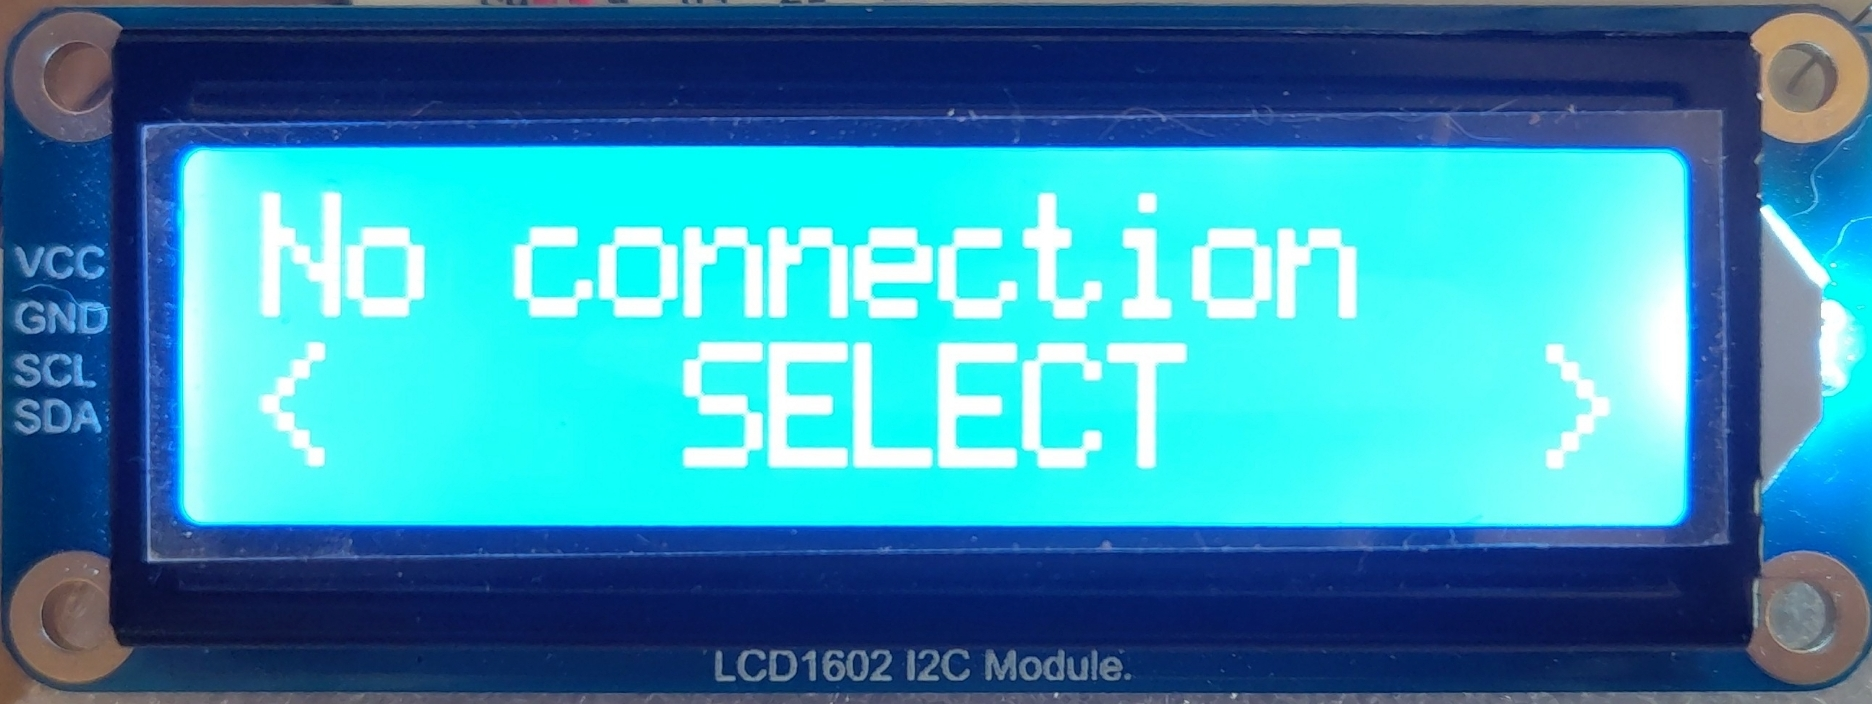
\includegraphics[width=0.55\textwidth]{images/device_ui_disconnected}
	\caption{Device UI when there are no active Bluetooth connections (see Appendix~\ref{appendix:ui_disconnected} for full size view)}
	\label{fig:ui_disconnected}
\end{figure}

\begin{figure}[H]
	\centering
	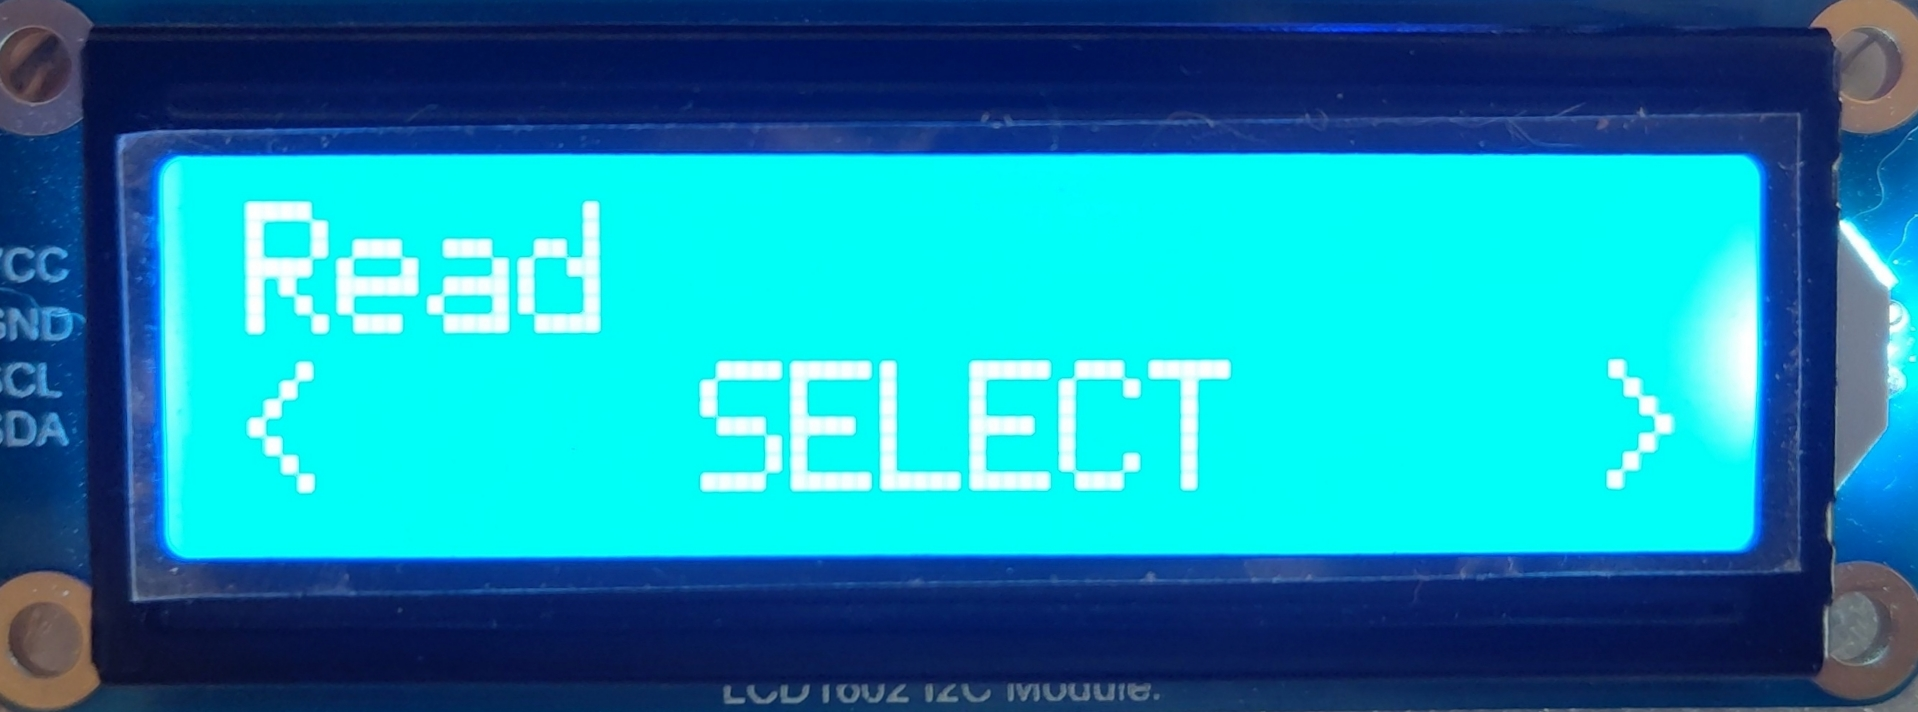
\includegraphics[width=0.55\textwidth]{images/device_ui_connected}
	\caption{Device UI when there are active Bluetooth connections (see Appendix~\ref{appendix:ui_connected} for full size view)}
	\label{fig:ui_connected}
\end{figure}

\begin{figure}[H]
	\centering
	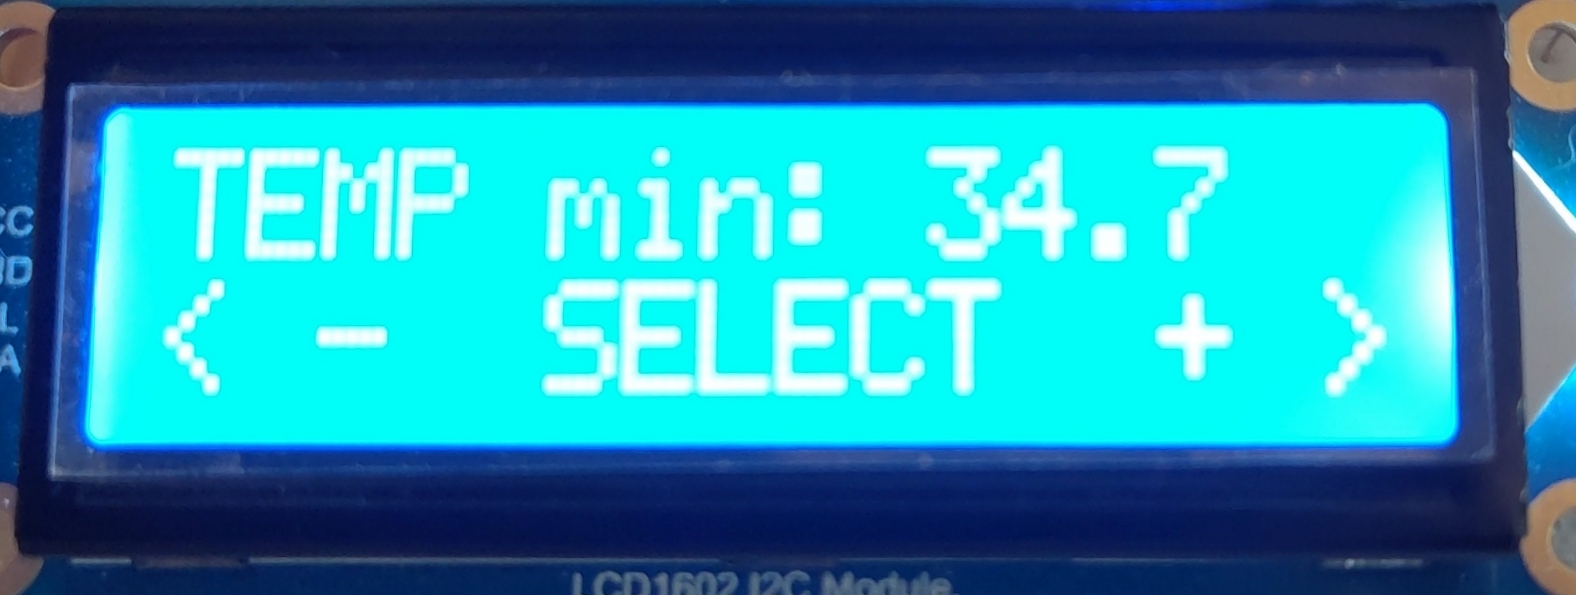
\includegraphics[width=0.55\textwidth]{images/device_ui_set_temp}
	\caption{Device UI when locally setting the temperature thresholds (see Appendix~\ref{appendix:ui_setup_temp} for full size view)}
	\label{fig:ui_set_temp}
\end{figure}

\subsubsection{Visual Feedback: Status Indicator LEDs}
Four LEDs are incorporated inside this device to give instantaneous, nonverbal feedback about connectivity and system status. Without looking at the LCD interface, users can rapidly determine operational conditions at a glance thanks to their clear and extremely simple nature. A different system state (not referring to states in the context of the state machine but rather operational conditions), such as regular operation, warnings, critical alerts, or connectivity status, is linked to each LED. By providing a quick overview of vital sign evaluations and device performance, this improves usability in clinical settings.

\subsubsection{Auditory Feedback: Buzzer}
Feedback is also provided by the buzzer on the device, for instance for abnormal measurements or any possible errors that may occur. For example, the buzzer emits certain tone patterns to notify either medical staff or the patient (if they have been released from hospital and are using the device for continuous at-home monitoring) if three consecutive read attempts are unsuccessful or if a vital sign reading deviates from permitted limits and must be transmitted. In situations where visual cues could be overlooked or are otherwise unavailable (e.g. if the patient is blind), the duality of having output both visually and audibly is vital.

The user interface design attempts to strike a balance between practicality and simplicity. It increases the system's dependability in a medical setting by reducing the need for user training and guaranteeing that important information is communicated quickly, while also providing the necessary functionality to control the system efficiently.

\section{Project Planning} % Section 3.6
To make sure that development, testing, and documentation progressed in a timely and systematic manner, the project execution was divided into distinct phases with some phases overlapping if it made sense to do so. The Gantt chart below shows the timeframe, which spans the months of October 2025 through May 2025. The pace and priority of the system's development and academic submission process are reflected in this timeline.

% \newgeometry{margin=1in}
\clearpage
\begin{landscape}
\vspace*{-1cm}
\begin{ganttchart}[
	hgrid,
	vgrid,
	time slot format=isodate-yearmonth,
	time slot unit=month,
	x unit=2.2cm,
	y unit chart=0.9cm,
	milestone label anchor/.append style={below=-1.6ex},
	milestone label font=\footnotesize\bfseries,
	bar label font=\normalsize\bfseries,
	bar/.append style={fill=blue!30},
	milestone/.append style={fill=red!70}
]{2024-10}{2025-05}

\gantttitlecalendar{year, month=shortname} \\

\ganttbar{Requirements Gathering}{2024-10}{2024-10} \\
\ganttbar{Literature Review}{2024-10}{2024-11} \\
\ganttbar{Hardware Design}{2024-12}{2025-04} \\
\ganttbar{Software Development}{2025-02}{2025-05} \\
\ganttbar{Thesis Writing}{2025-03}{2025-05} \\
\ganttbar{Testing and Debugging}{2025-04}{2025-05} \\
\ganttbar{Final Review \& Polish}{2025-05}{2025-05} \\
\ganttbar[bar/.append style={fill=green!70}]{Prototype Complete}{2025-05}{2025-05} \\
\ganttbar[bar/.append style={fill=blue!70}]{First Full Test}{2025-05}{2025-05} \\
\ganttbar[bar/.append style={fill=orange!60}]{Presentation}{2025-05}{2025-05} \\

\ganttnewline

\end{ganttchart}
\end{landscape}
\clearpage
% \restoregeometry


\begin{itemize}
	\item Gathering Requirements (October 2024): This initial phase concentrated on determining the system's objectives and functional requirements in light of postoperative care and Internet of Things-based medical monitoring.
	\item Review of Literature (October–November 2024): Research was done to comprehend the clinical and technical backdrop of vital sign monitoring systems, pertinent communication protocols, and medical device integration at the same time as requirements gathering.
	\item Hardware Design (December 2024–April 2025): This stage included choosing and integrating sensors, microcontrollers, and communication modules as well as designing and developing the device's electronics and circuit-level architecture.
	\item Software Development (February-May 2025): This stage, which overlapped with hardware design, concentrated on developing the Arduino-based system's firmware, putting state logic into practice, and providing preliminary support for receiving and transmitting sensor data.
	\item Thesis Writing (March–May 2025): As development stabilised, the thesis's composition and writing got underway. This made it possible to provide actual implementation information, system schematics, and assessment findings.
	\item Testing and Debugging (April–May 2025): This step involved testing system module integration, validating state transitions, and improving threshold configuration and error-handling procedures all at the same time as documentation.
	\item Thesis Final Evaluation and Polishing (May 2025): With the help of my supervisors, revisions were made to the thesis, and mistakes corrected.
	\item First complete version finalised (May 2025): First completely working version done and ready for full testing.
	\item Presentation (May 2025): Visual aids and practice sessions for the project's final presentation.
\end{itemize}

\section{Summary} % Section 3.7
This section described the full foundational design of the system being developed, starting with an assessment of the user and technical requirements. These served as a guide for overall development and were drawn from the practical demands of postoperative patient care.

The interactions between patients, medical personnel, and the system were made clear by the use case diagram. This section also highlighted the ways in which data is gathered, sent, and examined. The architecture of the system, including high-level data flow and hardware integration, was discussed introducing the main technological elements such as the LoRaWAN communication backbone and the microcontroller-based circuit architecture. Following that, the user interface design was discuseed in detail, analysing the function and reasoning behind the LEDs, the LCD screen, the buttons, and the buzzer. The project's development cycle was finally depicted by a Gantt chart, which demonstrated how the many design and implementation phases were arranged and overlapped to effectively fulfil deadlines. When combined, these components create a coherent and well-designed system that meets the specified technological and practical objectives while retaining extensibility and adaptability for future modifications.


\chapter{Implementation and Testing}

\section{Introduction}
Introduce what this chapter is going to present.
\section{Implementation}

\subsection{Next subsection}

\subsection{Next subsection}

\section{Testing}

\subsection{Next subsection}

\subsection{Next subsection}

\section{Summary}
Summarise what was said in this chapter and link with the next chapter.

\chapter{Discussion}

\section{Introduction}
Introduce what this chapter is going to present.
\section{Discussion}

\section{Difficulties phased}

\section{Knowledge acquired}

\section{Future work}

\section{Conclusions}


% \chapter*{Bibliography}
\addcontentsline{toc}{chapter}{Bibliography}

\addcontentsline{toc}{chapter}{References}
\renewcommand{\bibname}{References}
\bibliographystyle{IEEEtran}
\bibliography{references}

\chapter*{Appendices}
\addcontentsline{toc}{chapter}{Appendices}

\section*{Appendix A}
\addcontentsline{toc}{section}{Appendix A}

\begin{landscape}
\begin{figure}[H]
	\centering
	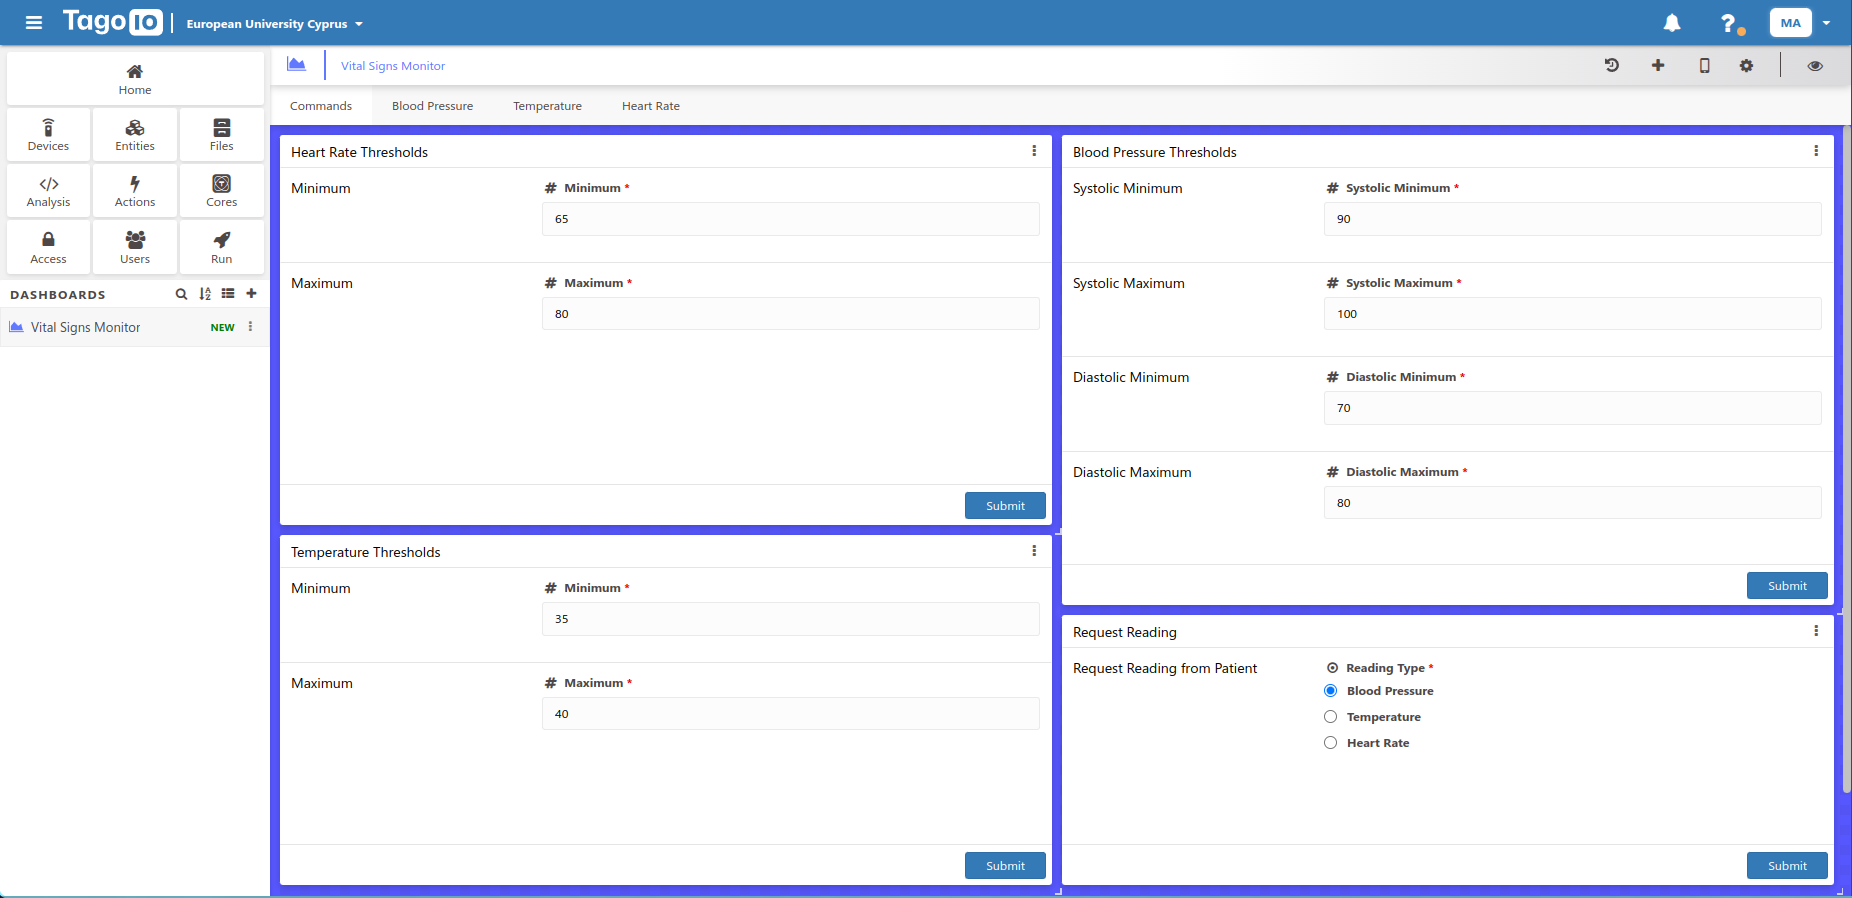
\includegraphics[width=\linewidth]{images/tagoio_dashboard_cmds}
	\caption{TagoIO dashboard: Commands pannel for remote requests and thresholds setting}
	\label{appendix:tagoio_commands}
\end{figure}
\end{landscape}

\newpage
\begin{landscape}
\begin{figure}[H]
	\centering
	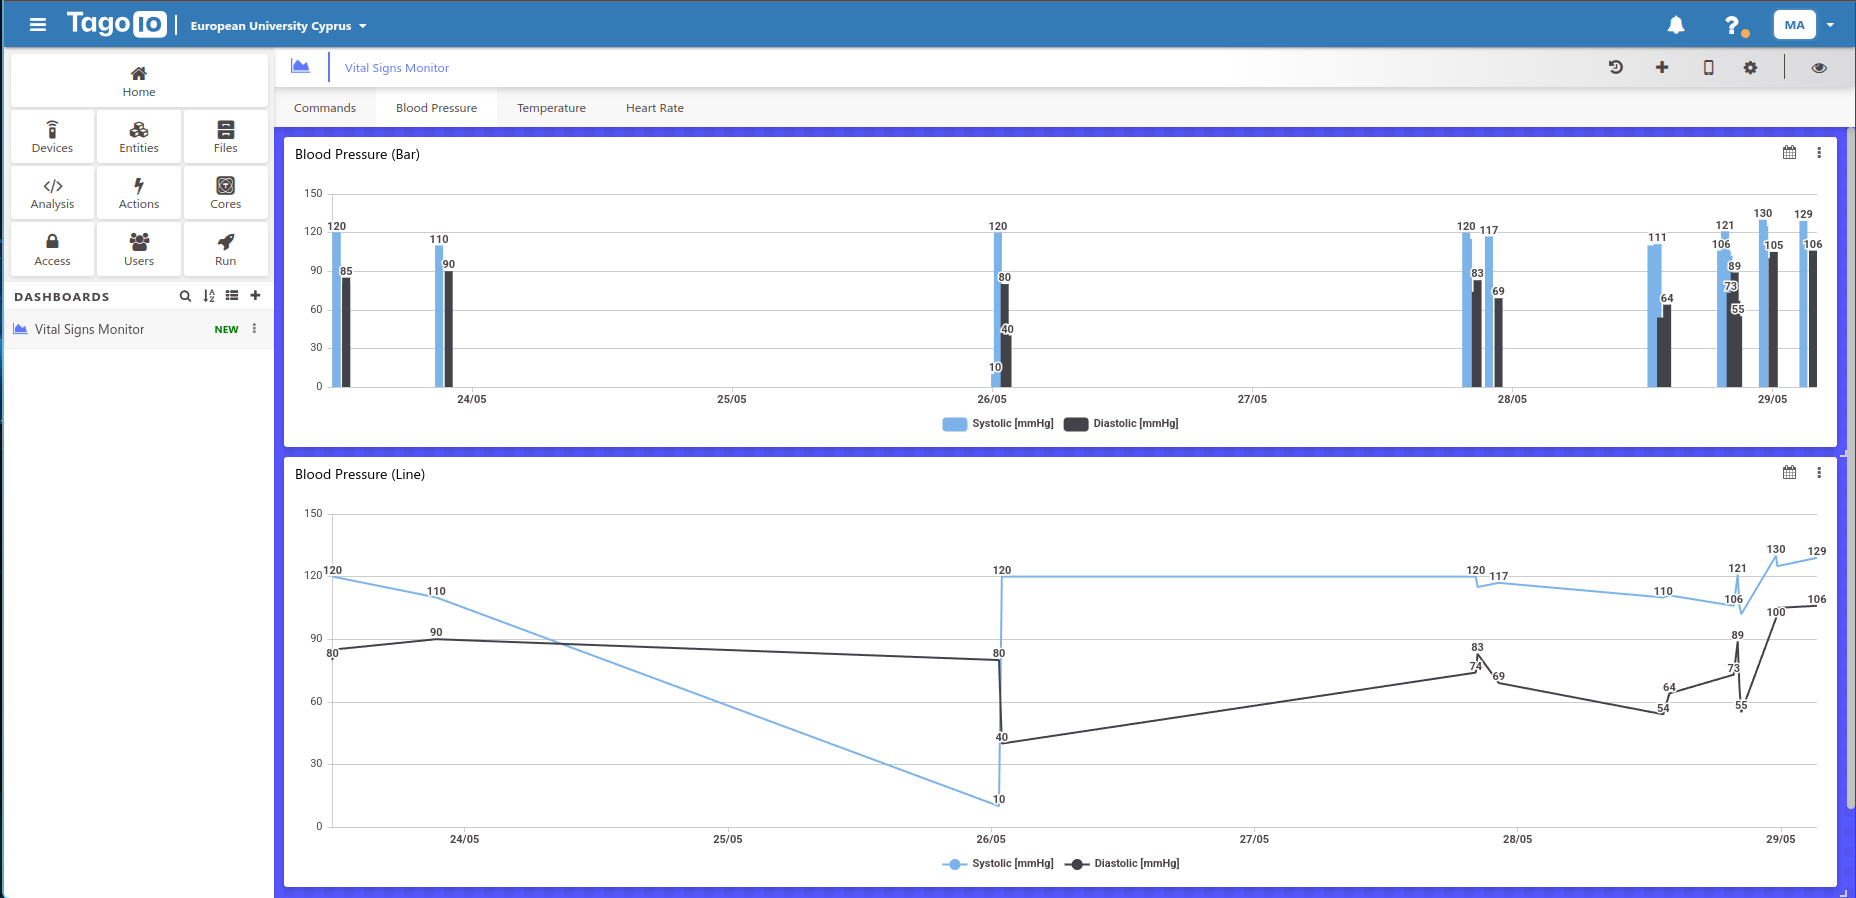
\includegraphics[width=\linewidth]{images/tagoio_dashboard_bp}
	\caption{TagoIO dashboard: Blood pressure visualisation panel}
	\label{appendix:tagoio_bp}
\end{figure}
\end{landscape}

\newpage
\begin{landscape}
\begin{figure}[H]
	\centering
	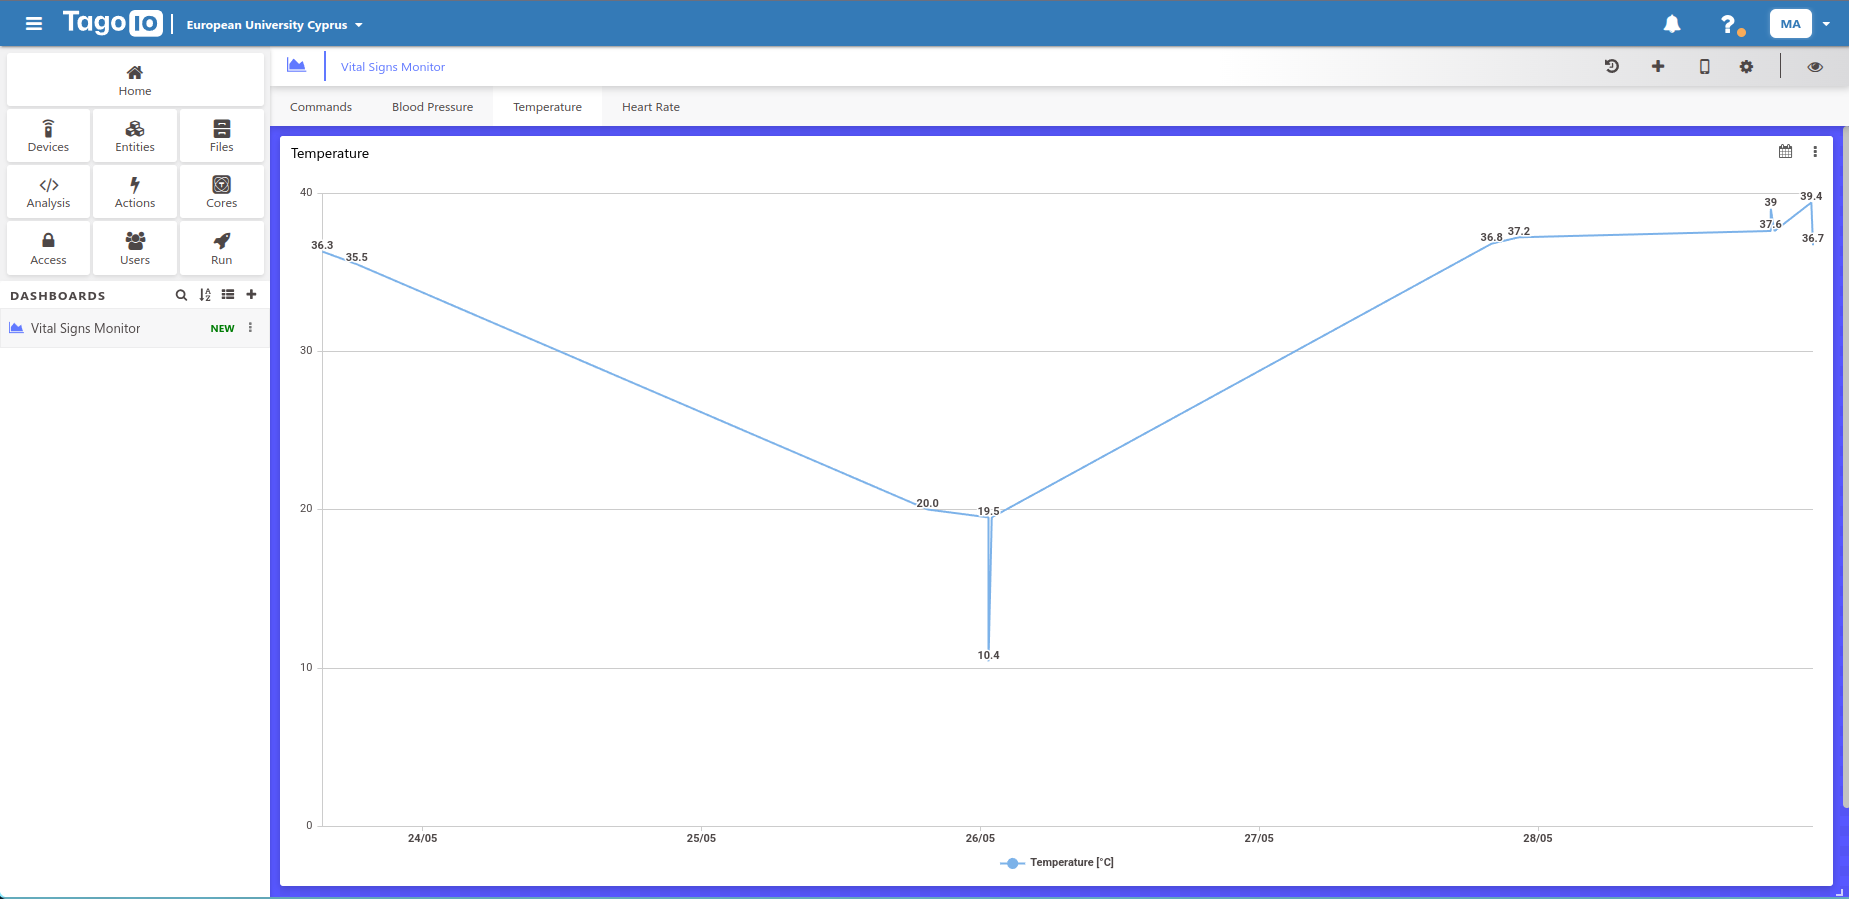
\includegraphics[width=\linewidth]{images/tagoio_dashboard_temp}
	\caption{TagoIO dashboard: Temperature visualisation panel}
	\label{appendix:tagoio_temp}
\end{figure}
\end{landscape}

\newpage
\begin{landscape}
\begin{figure}[H]
	\centering
	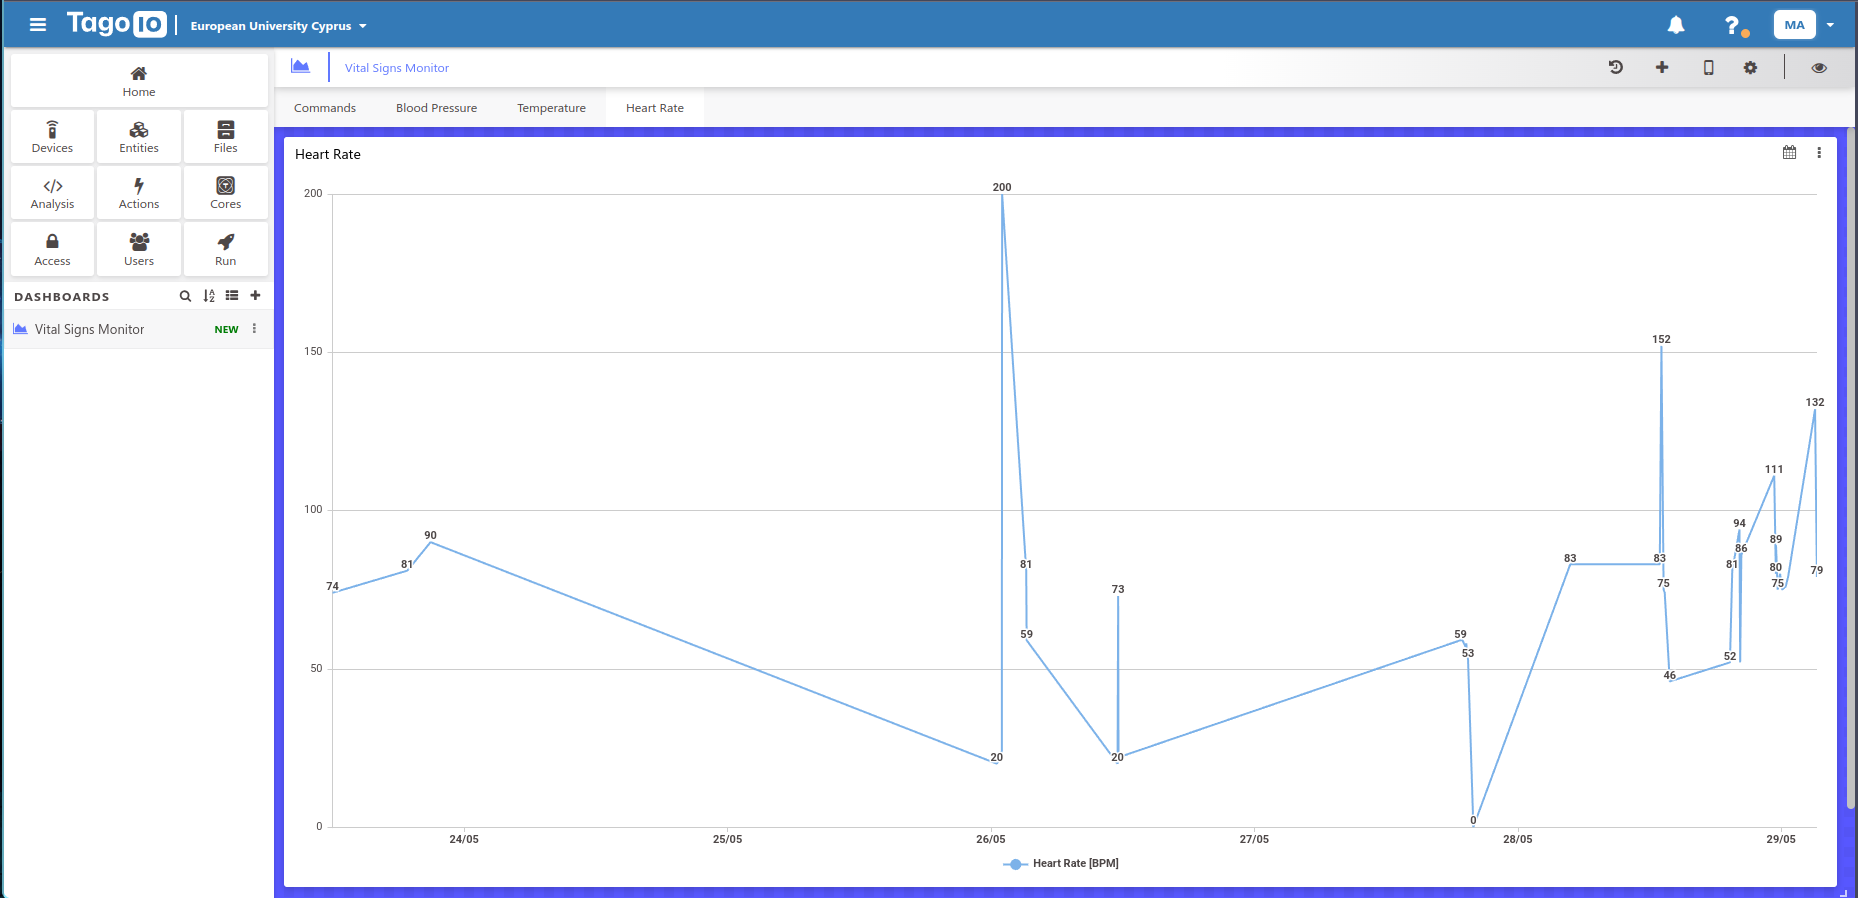
\includegraphics[width=\linewidth]{images/tagoio_dashboard_hr}
	\caption{TagoIO dashboard: Heart rate visualisation panel}
	\label{appendix:tagoio_hr}
\end{figure}
\end{landscape}

\newpage
\begin{landscape}
\begin{figure}[H]
	\centering
	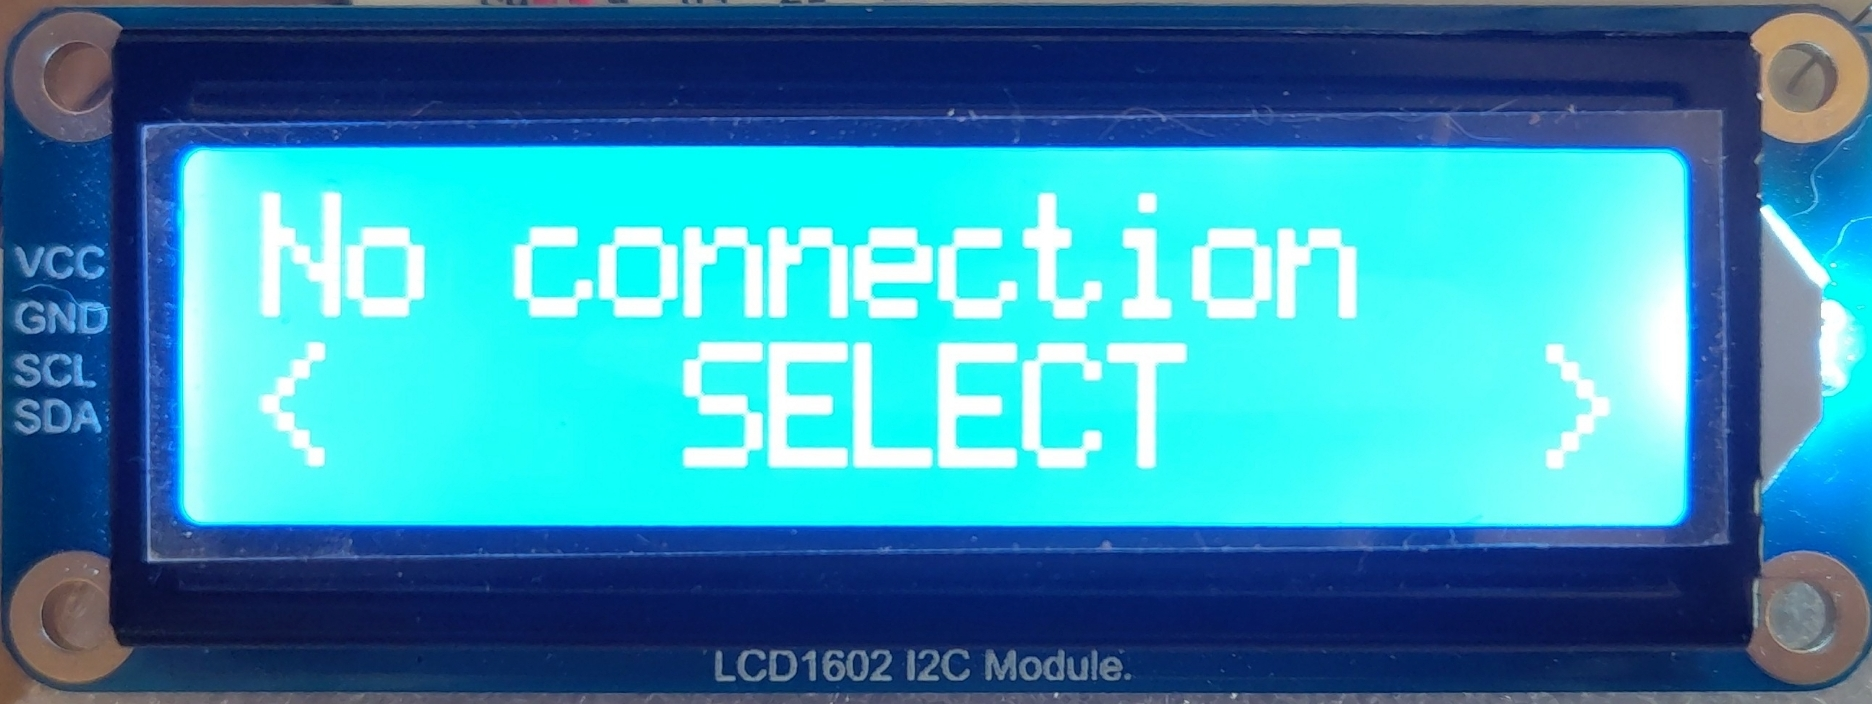
\includegraphics[width=\linewidth]{images/device_ui_disconnected.jpg}
	\caption{Full-size view of device LCD in DISCONNECTED state}
	\label{appendix:ui_disconnected}
\end{figure}
\end{landscape}

\newpage
\begin{landscape}
\begin{figure}[H]
	\centering
	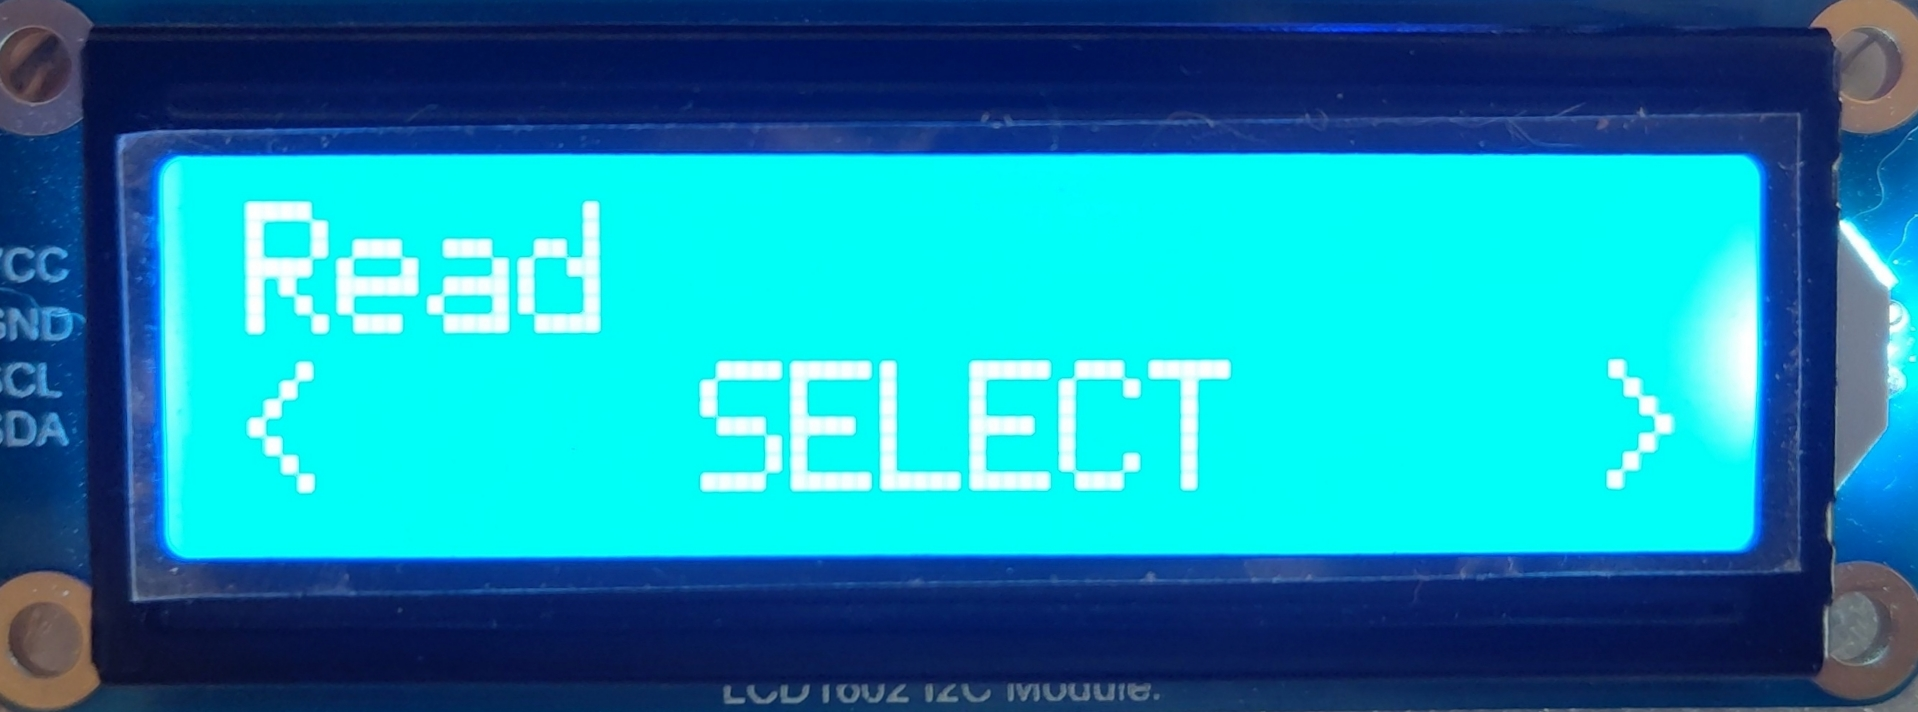
\includegraphics[width=\linewidth]{images/device_ui_connected.jpg}
	\caption{Full-size view of device LCD in CONNECTED state}
	\label{appendix:ui_connected}
\end{figure}
\end{landscape}

\newpage
\begin{landscape}
\begin{figure}[H]
	\centering
	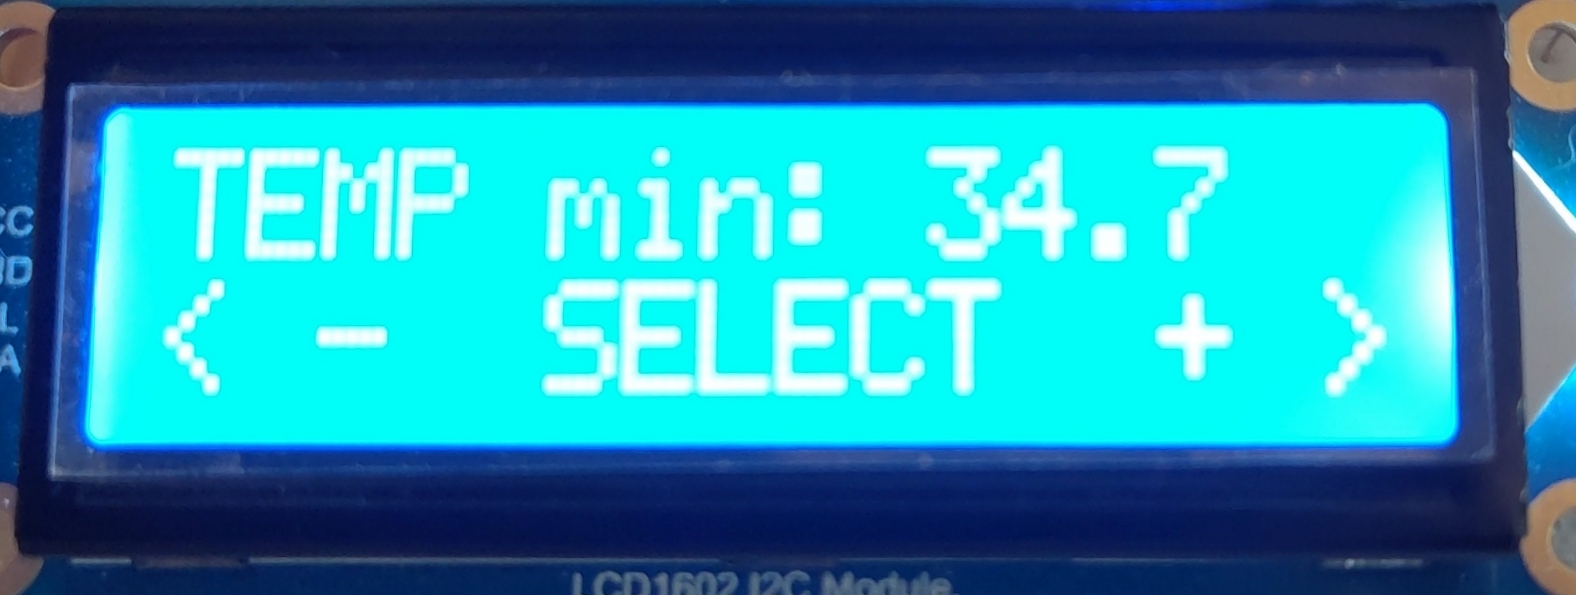
\includegraphics[width=\linewidth]{images/device_ui_set_temp.jpg}
	\caption{Full-size view of device LCD in SETUP\_TEMP configuration substate}
	\label{appendix:ui_setup_temp}
\end{figure}
\end{landscape}

% \newpage
\begin{figure}[H]
	\centering
	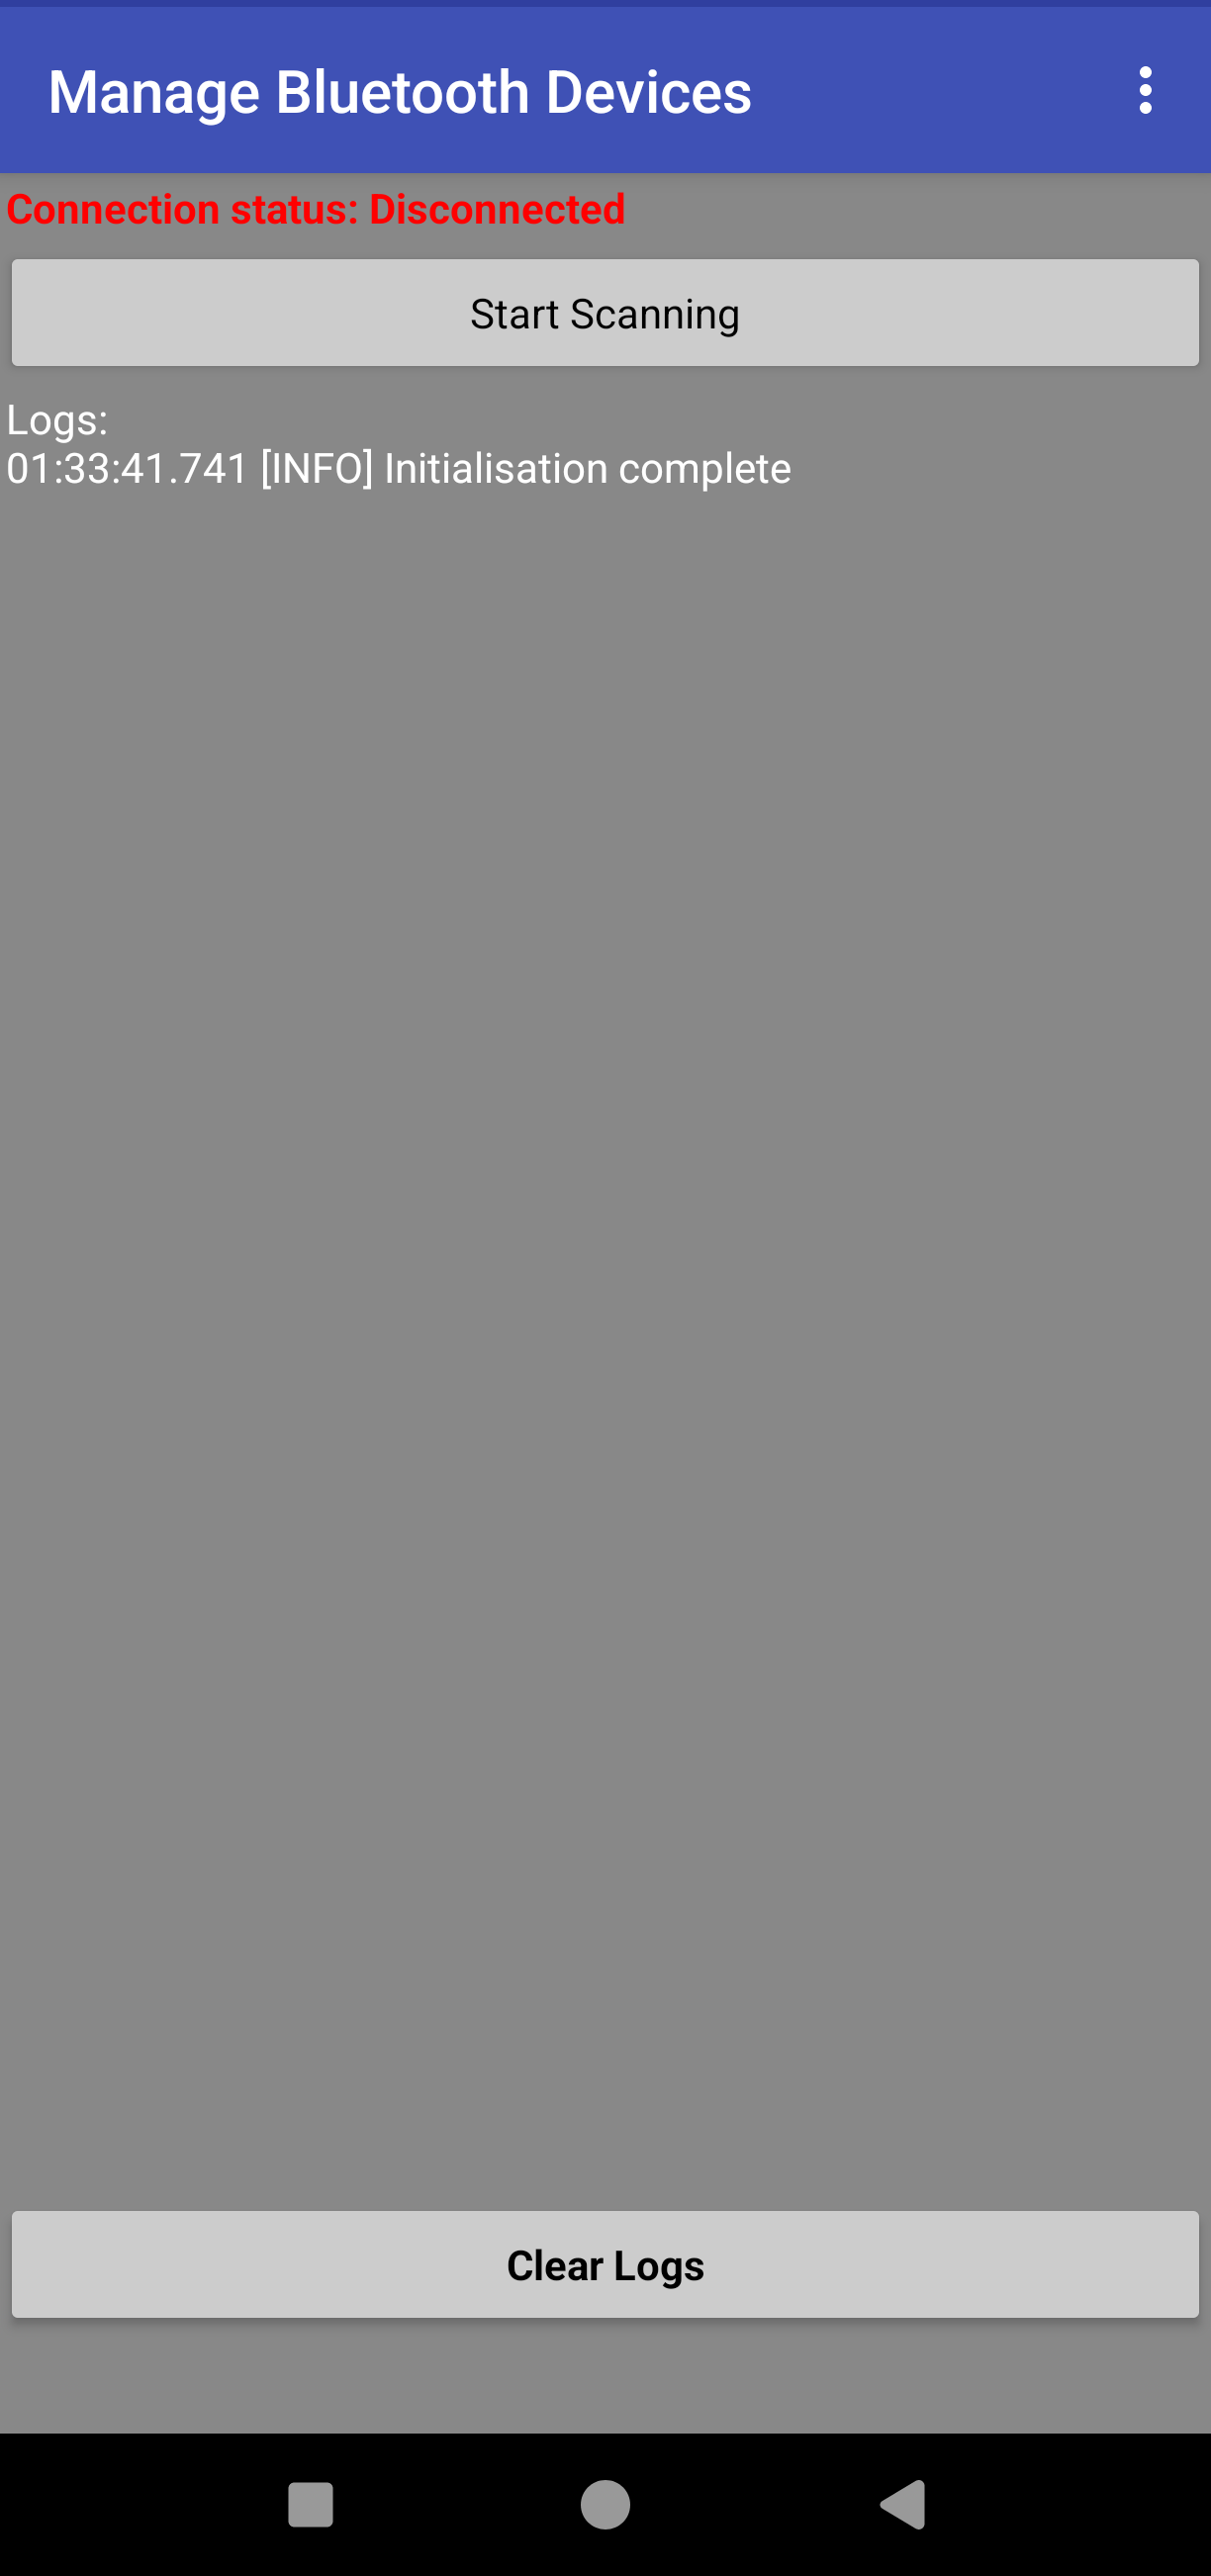
\includegraphics[width=0.7\textwidth]{images/app_ui_main_disconnected}
	\caption{App UI: First screen visible when starting the app}
	\label{appendix:app_ui_disconnected}
\end{figure}

\newpage
\begin{figure}[H]
	\centering
	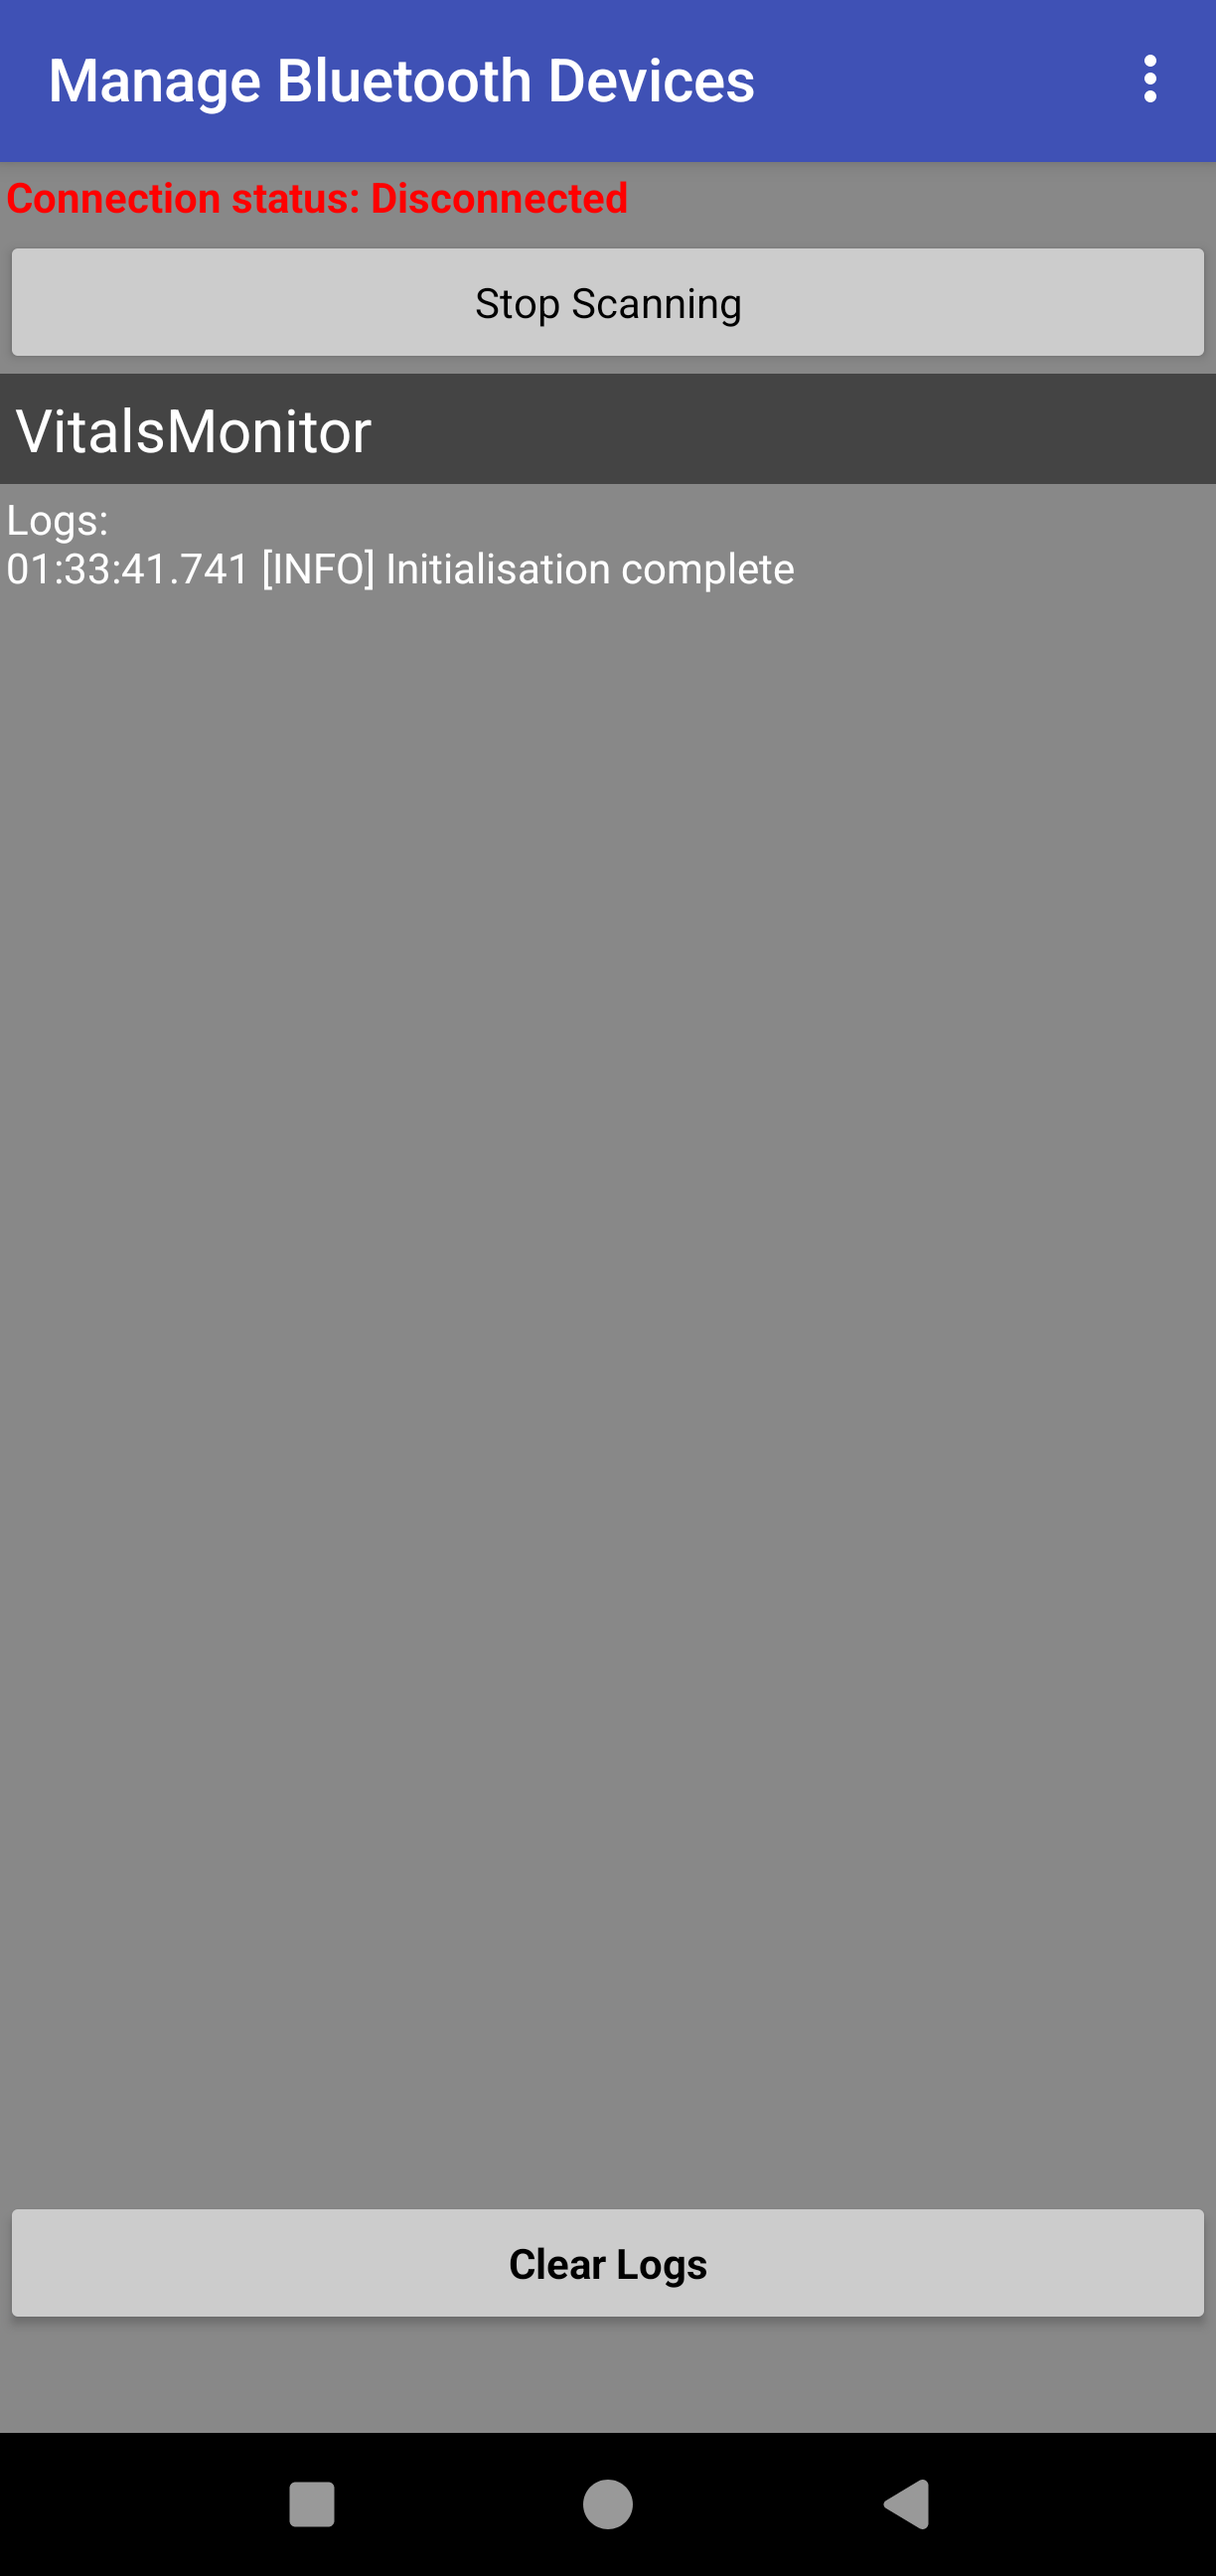
\includegraphics[width=0.7\textwidth]{images/app_ui_main_scanning}
	\caption{App UI: Screen when scanning for available Bluetooth devices}
	\label{appendix:app_ui_scanning}
\end{figure}

\newpage
\begin{figure}[H]
	\centering
	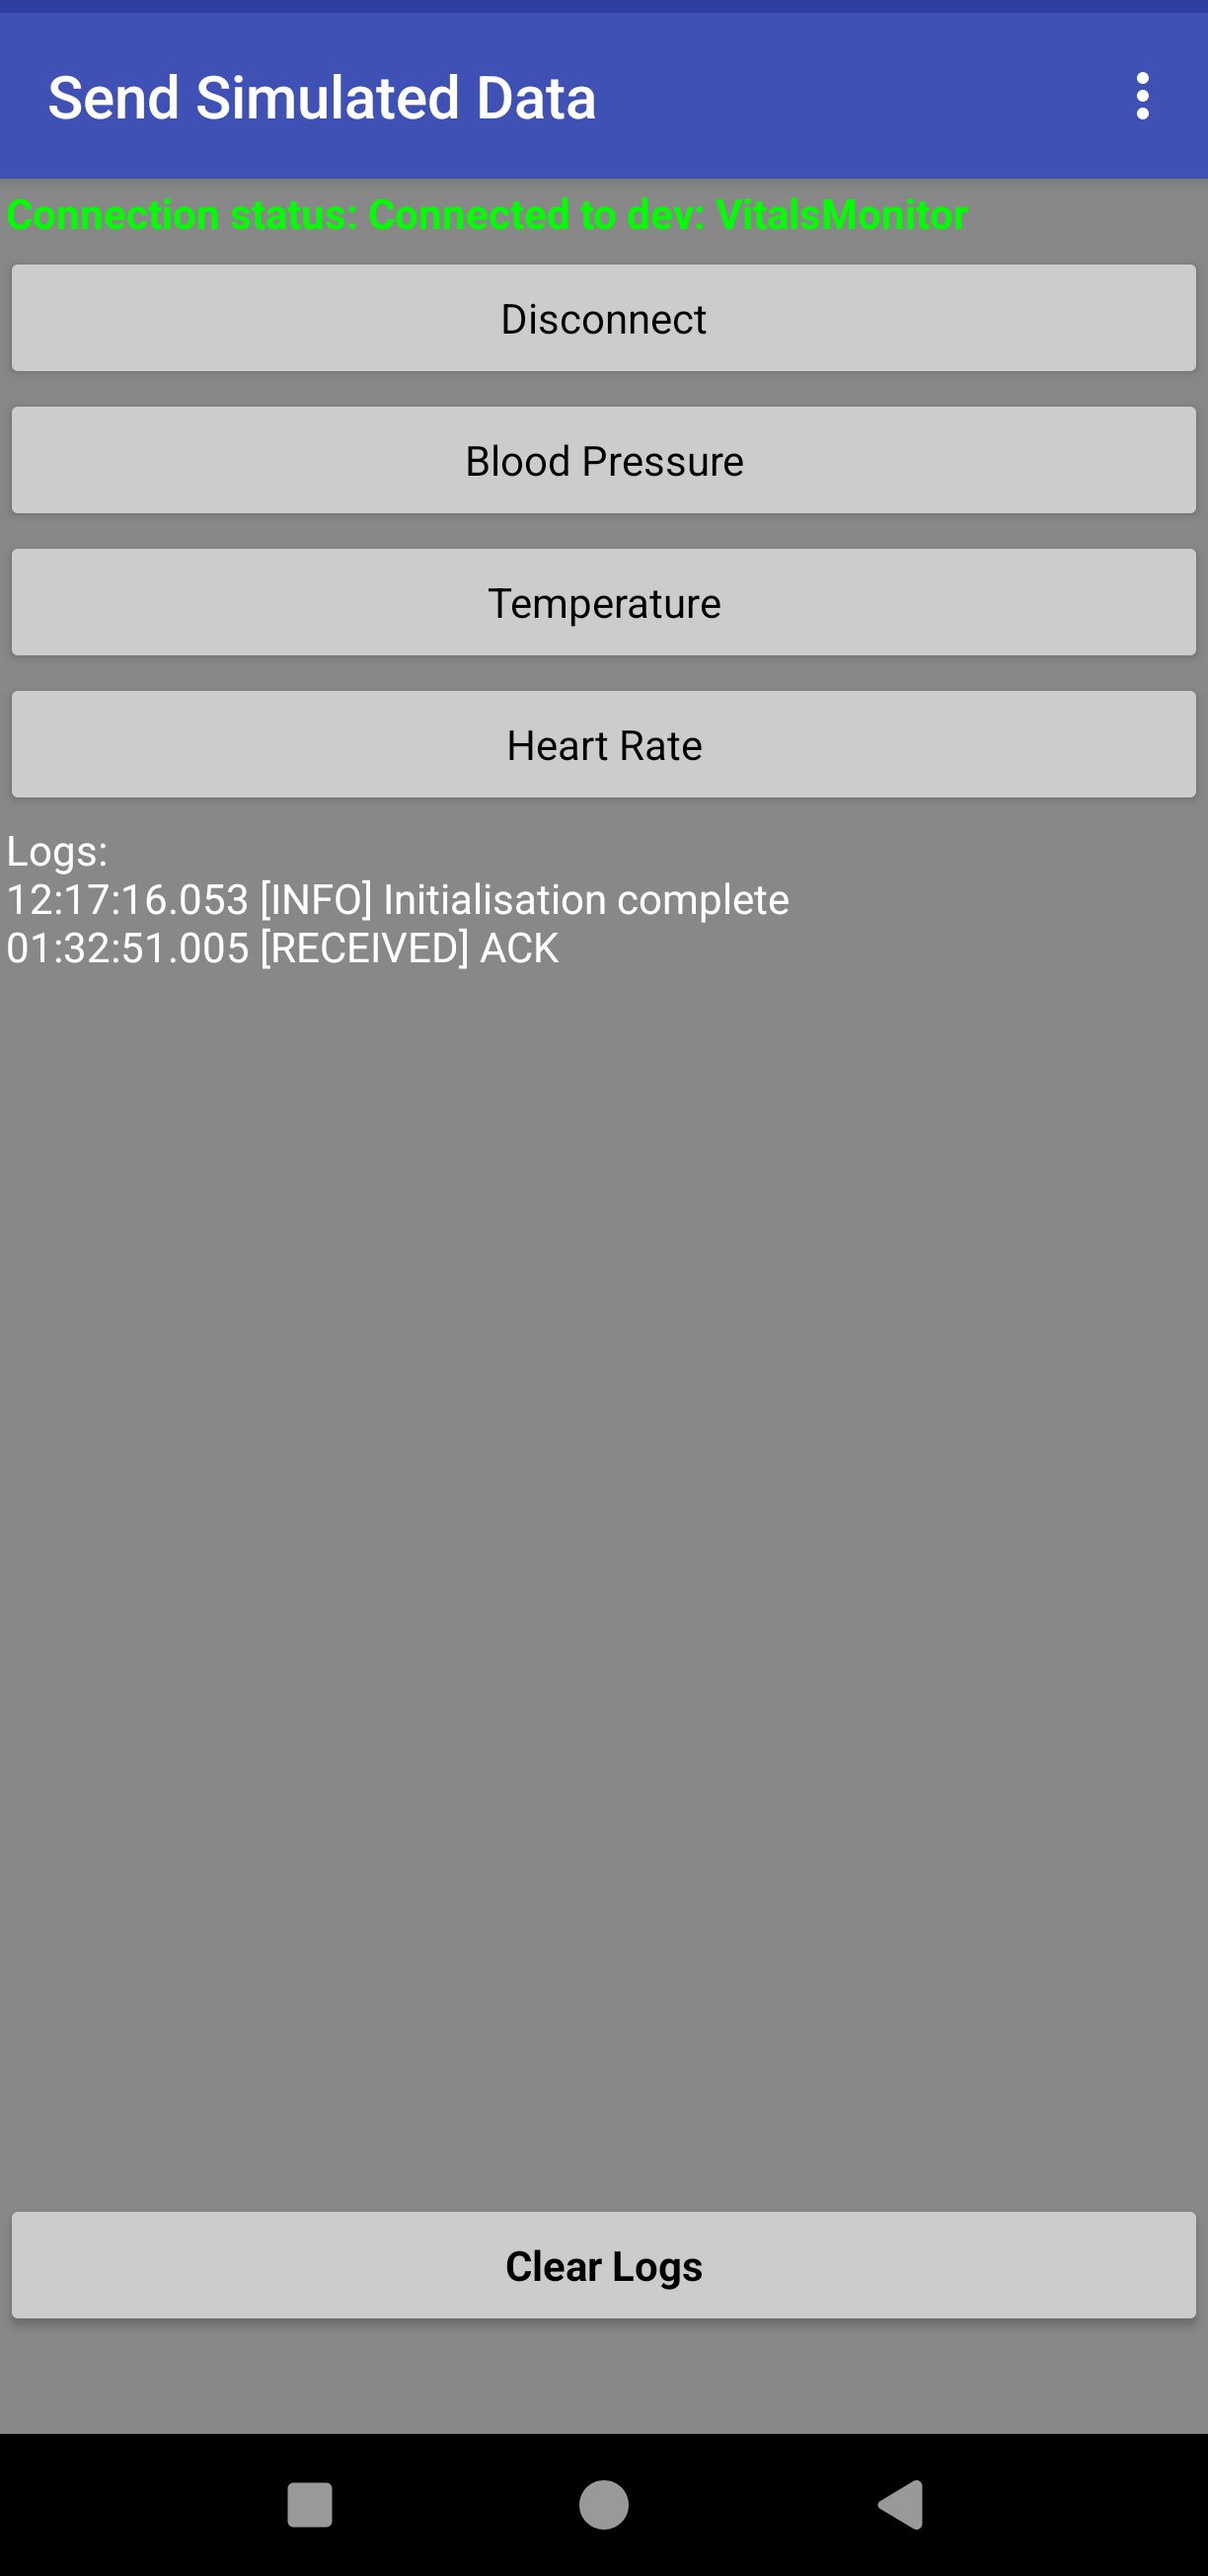
\includegraphics[width=0.7\textwidth]{images/app_ui_main_connected}
	\caption{App UI: Screen that is shown after a successful connection is established}
	\label{appendix:app_ui_connected}
\end{figure}

\newpage
\begin{figure}[H]
	\centering
	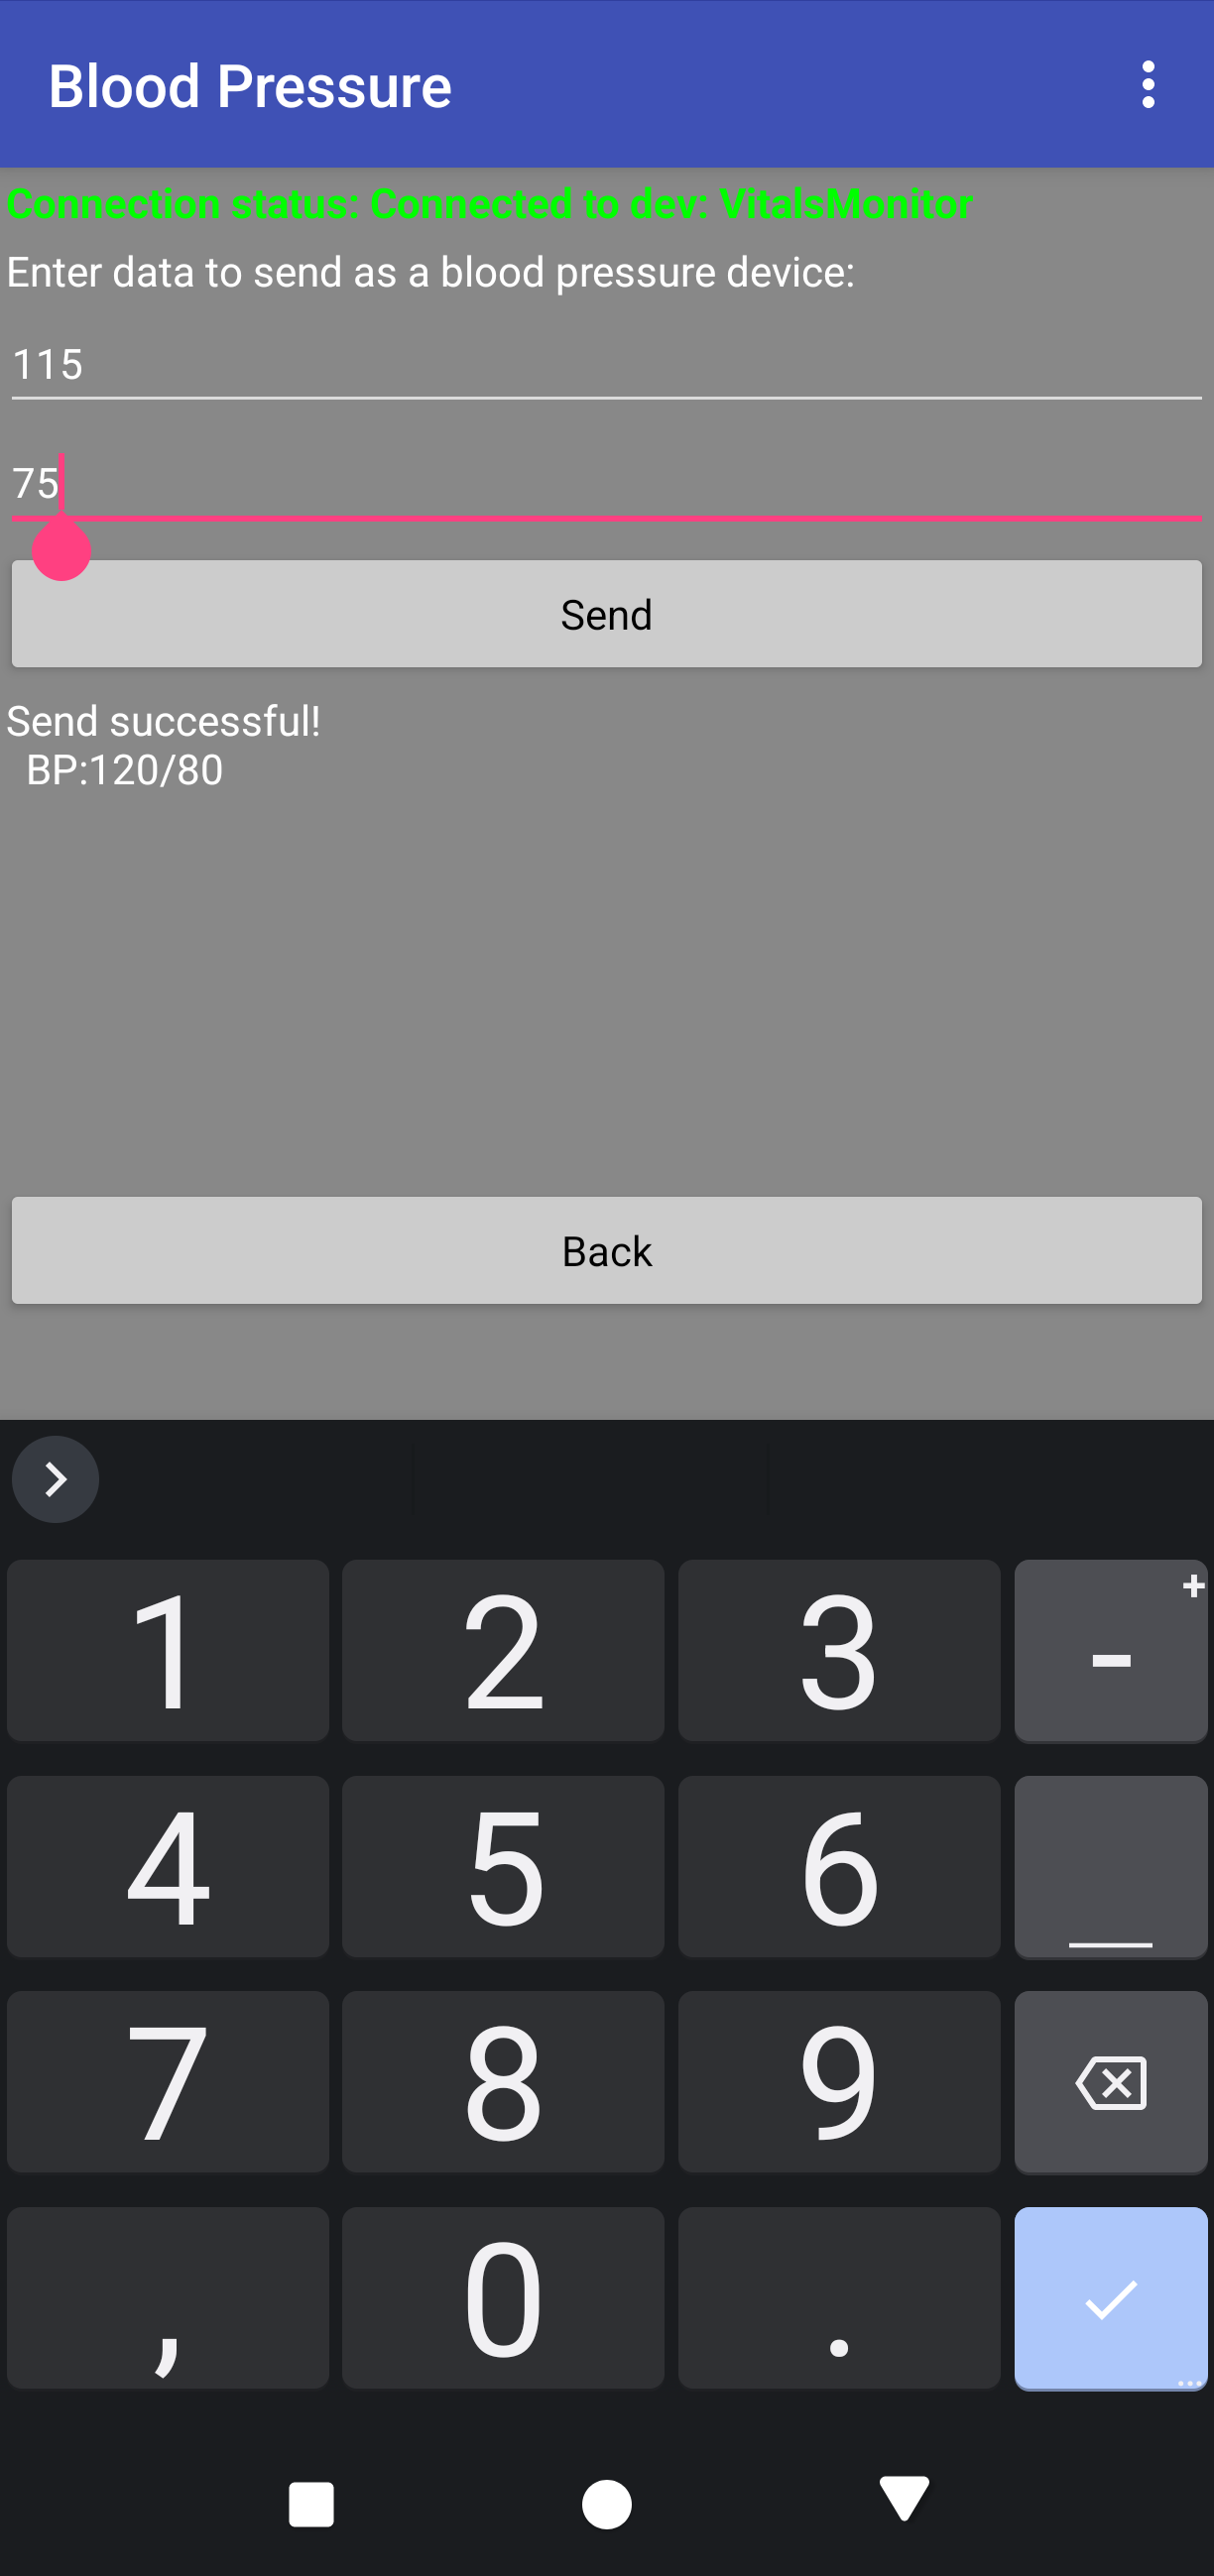
\includegraphics[width=0.7\textwidth]{images/app_ui_send_bp}
	\caption{App UI: Screen to send blood pressure data}
	\label{appendix:app_ui_bp}
\end{figure}

\newpage
\begin{figure}[H]
	\centering
	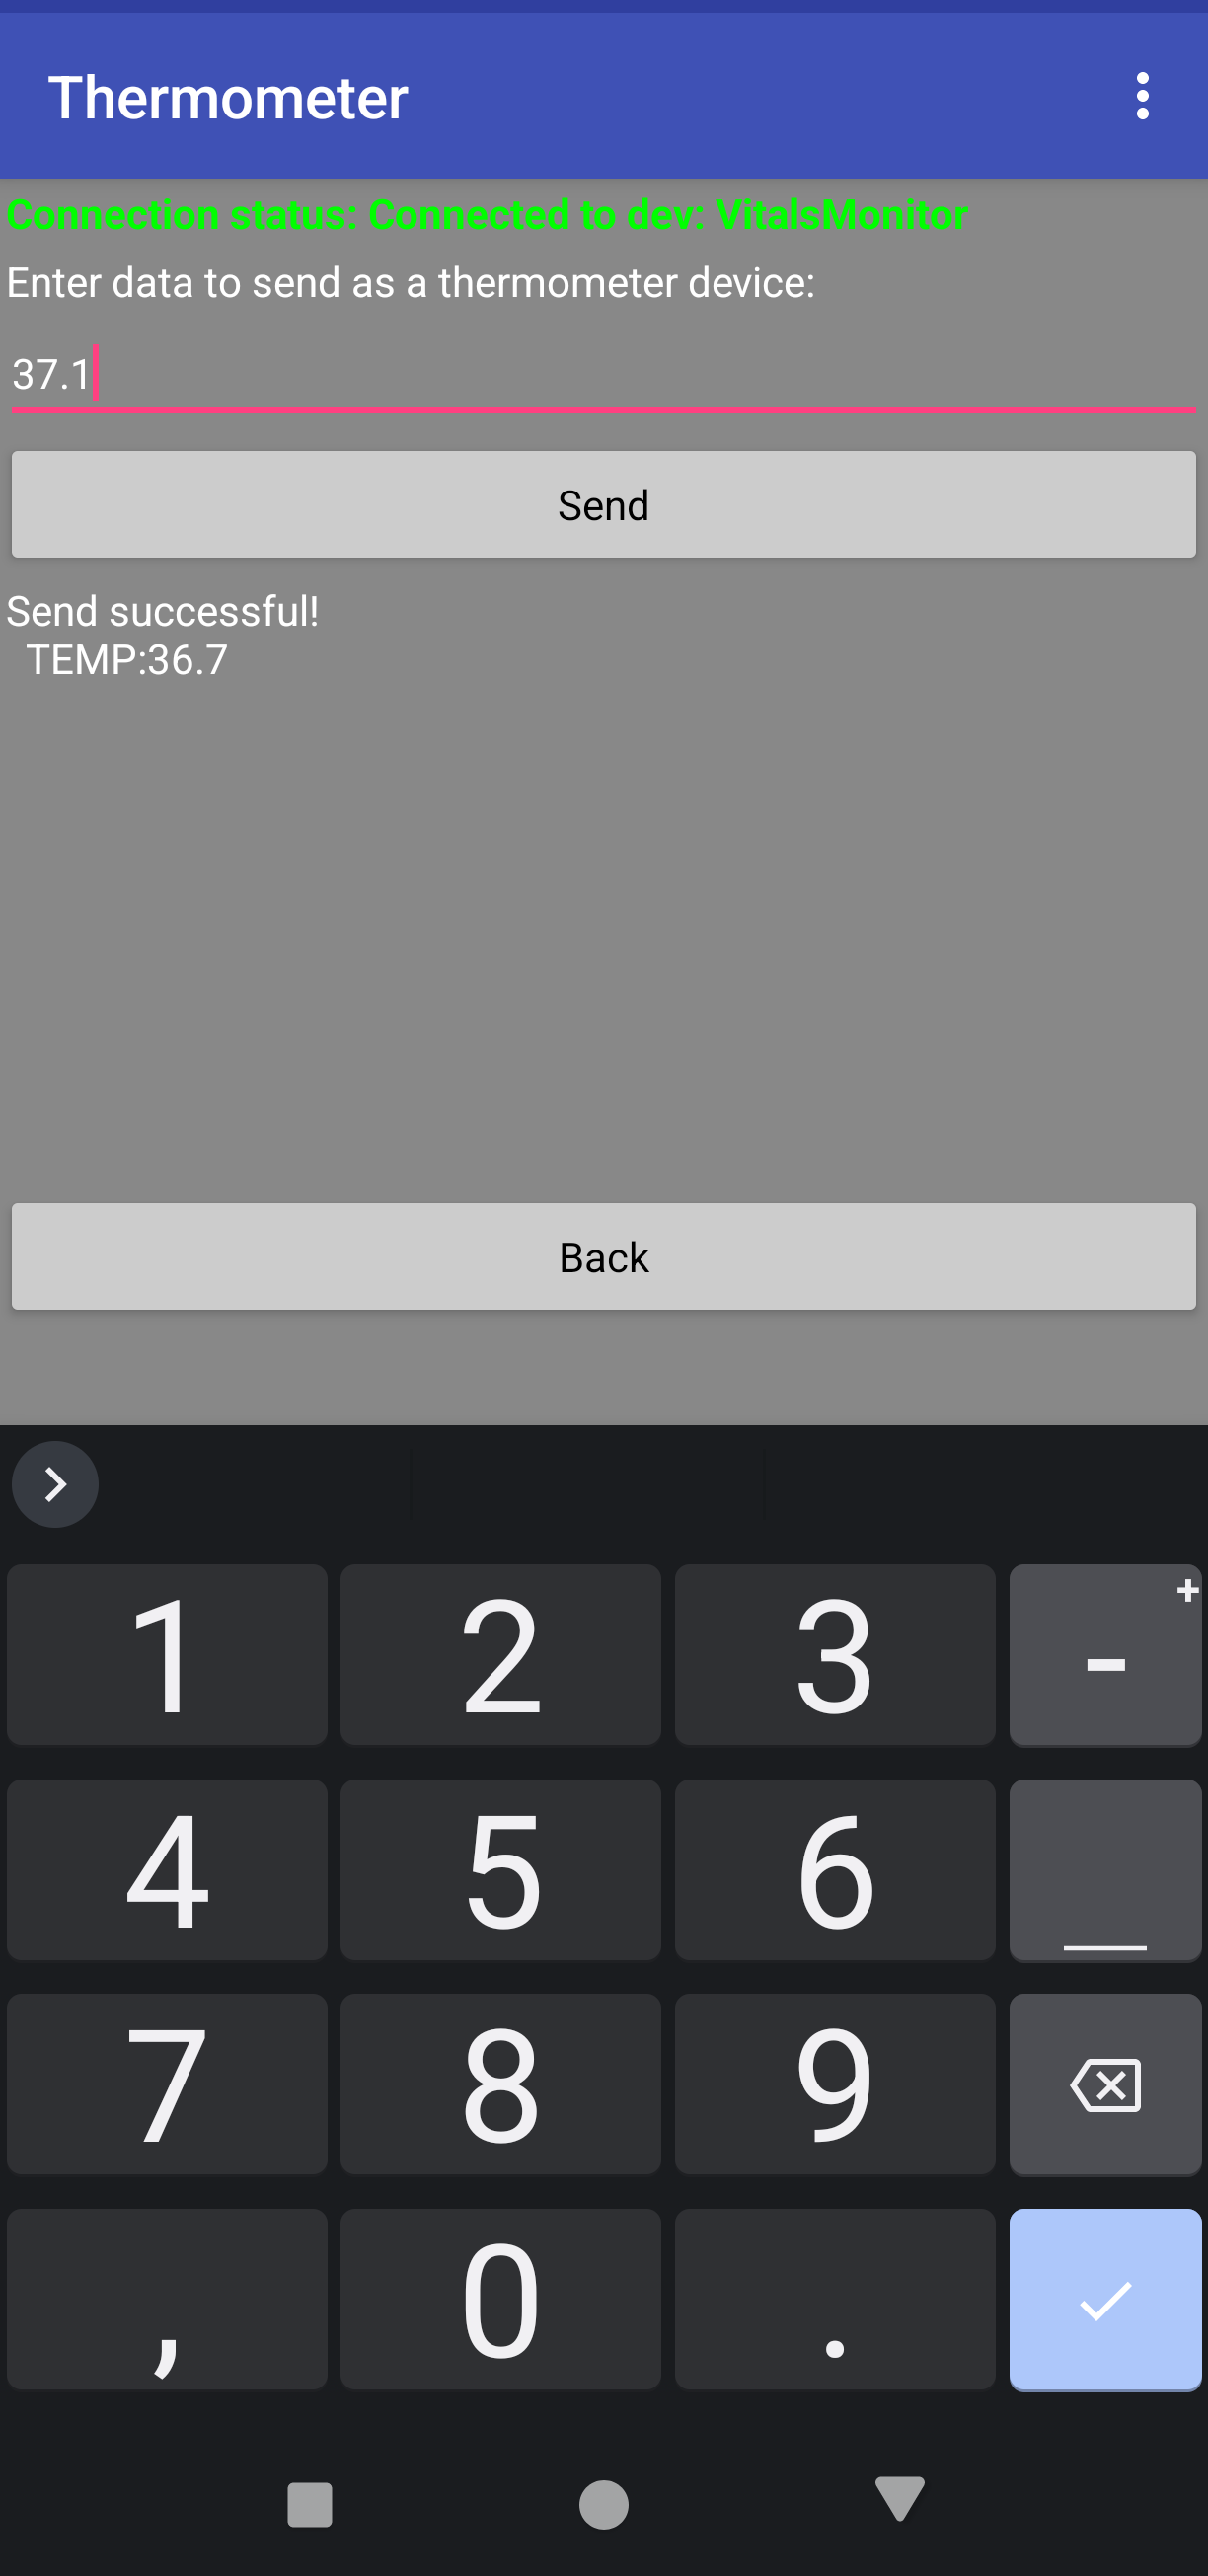
\includegraphics[width=0.7\textwidth]{images/app_ui_send_temp}
	\caption{App UI: Screen to send temperature data}
	\label{appendix:app_ui_temp}
\end{figure}

\newpage
\begin{figure}[H]
	\centering
	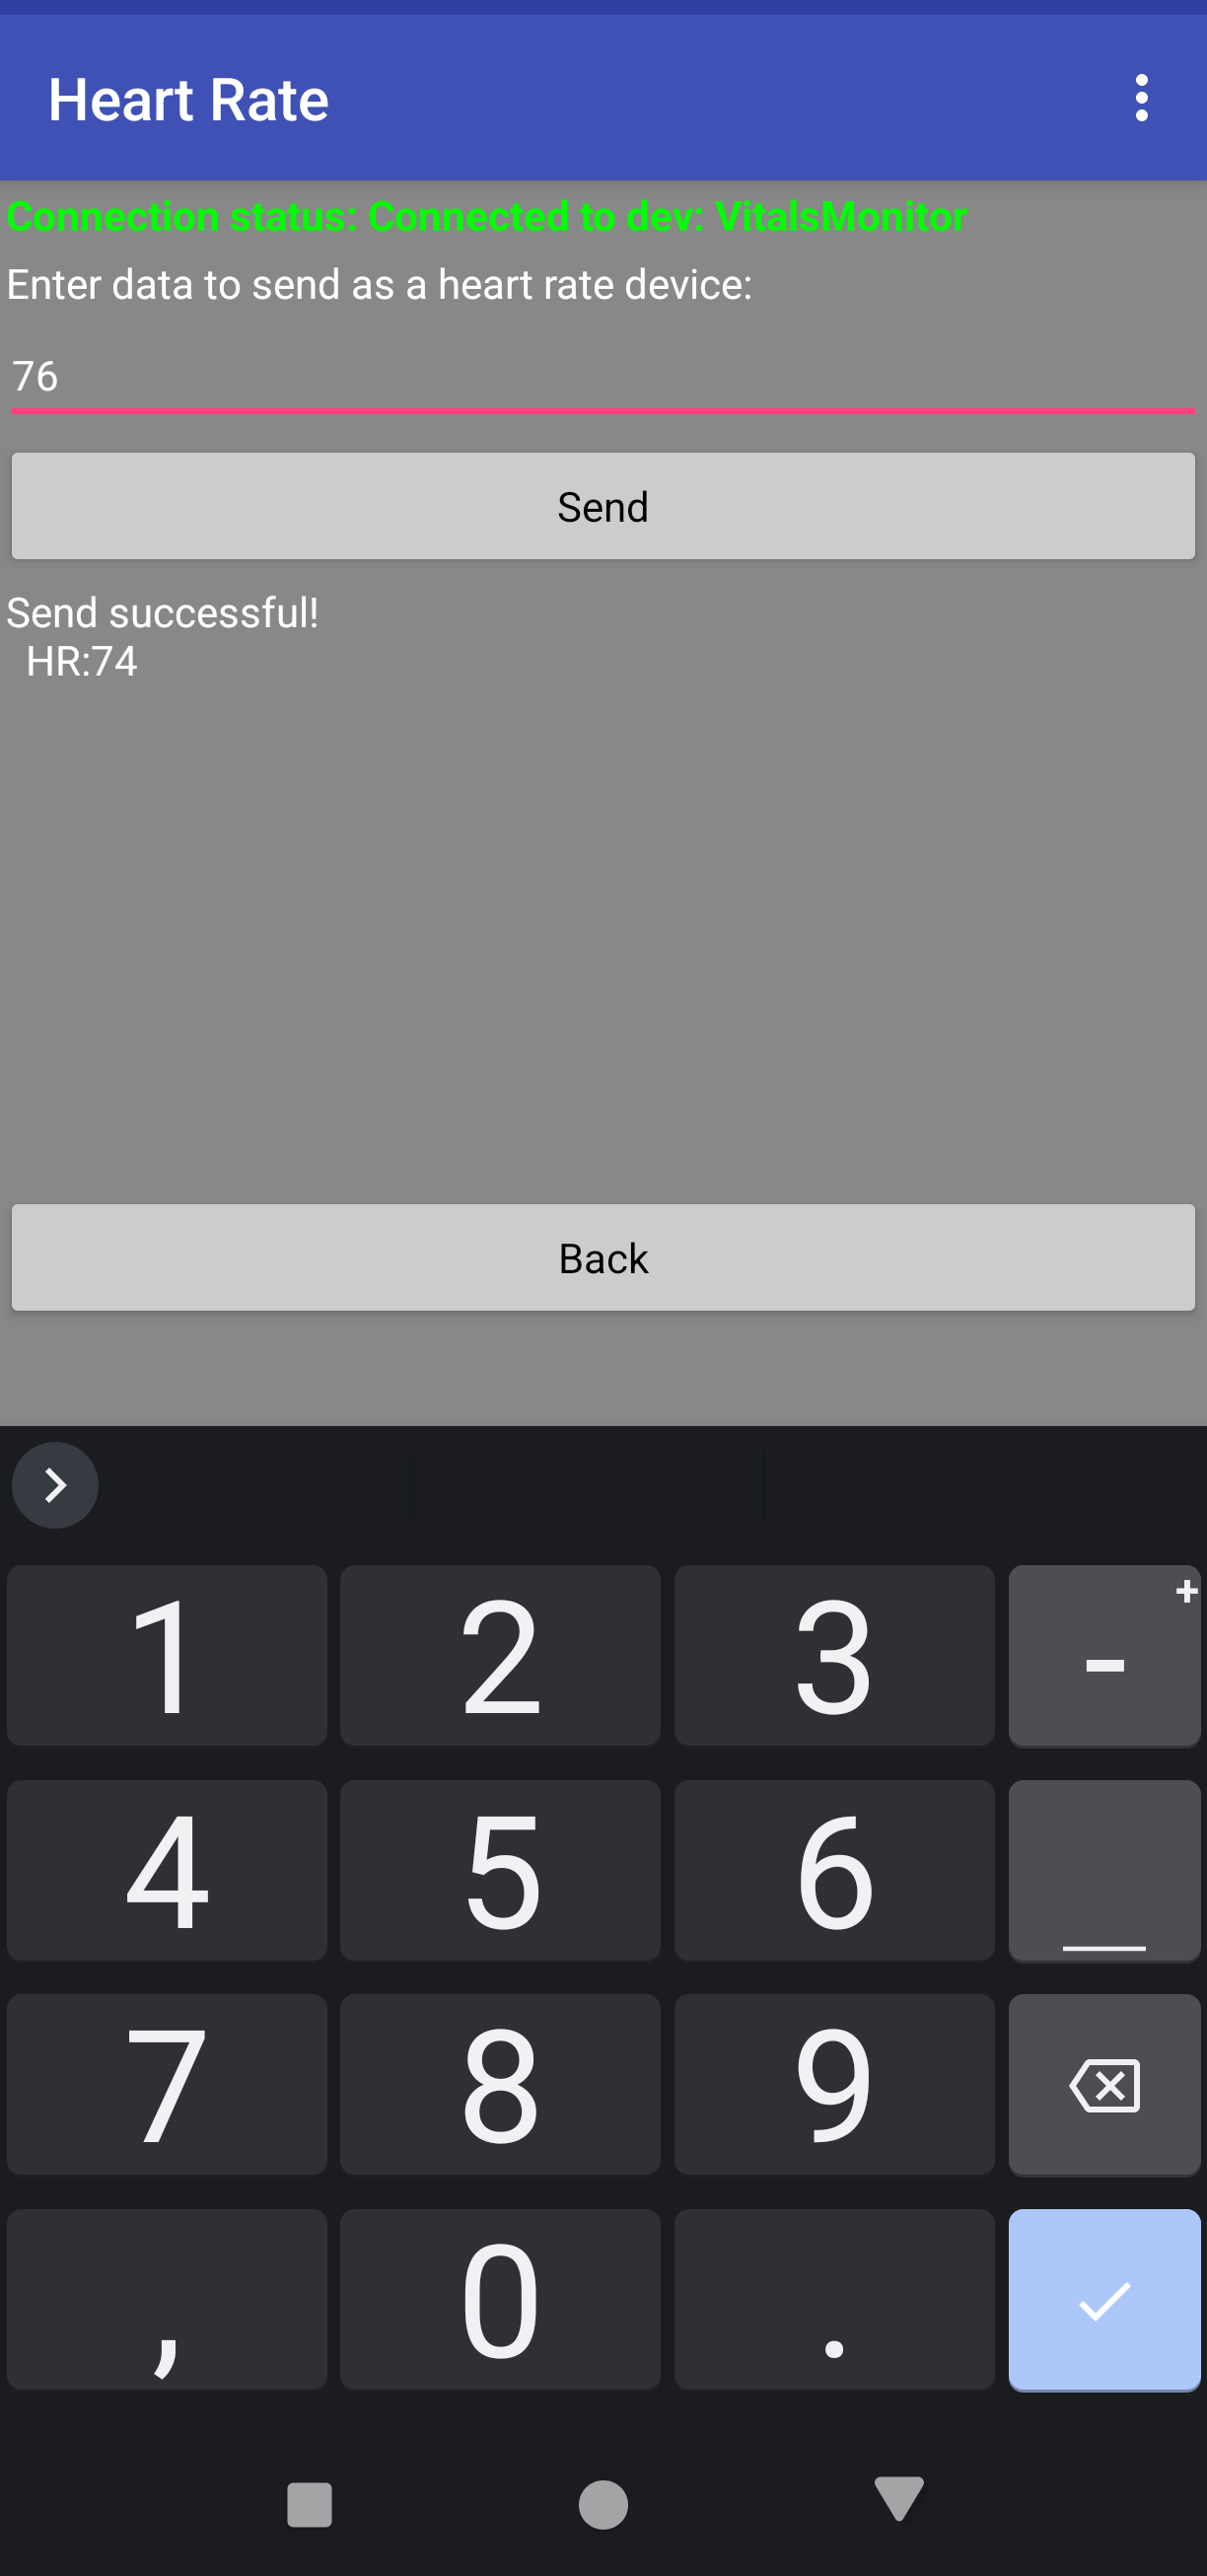
\includegraphics[width=0.7\textwidth]{images/app_ui_send_hr}
	\caption{App UI: Screen to send heart rate data}
	\label{appendix:app_ui_hr}
\end{figure}

% \newpage
% \section*{Appendix B}
% \addcontentsline{toc}{section}{Appendix B}
% Write a few words about the contents of the appendix


\chapter*{Manuals}
\addcontentsline{toc}{chapter}{Manuals}

\section*{User Manual}
\addcontentsline{toc}{section}{User Manual}
\paragraph{This device is designed to collect key health metrics in the post-operative phase via Bluetooth, and help you and your medical professionals monitor said vital signs. The three measurements it is capable of collecting and monitoring currently are blood pressure, temperature, and heart rate. It allows setting ranges for each metric, so that if a reading is outside these ranges it can automatically send it to the cloud and alert your medical professionals in order to allow them to more efficiently take care of you.}

\subsection{Getting Started}
\subsubsection{Power On}
\begin{itemize}
	\item Plug in device or add 6xAA standard batteries
	\item The LCD display will briefly display a message informing you it is booting, followed by "No connection" if there is no device currently set to auto-connect within Bluetooth range, or "Read" if there is a device within range and it automatically connects.
	% TODO: Add pictures of each screen under the correct bullet point
\end{itemize}

\subsection{Menu Navigation}
\subsubsection{Buttons}
\begin{itemize}
	\item \textbf{Prev} (left)
	\item \textbf{Select} (middle)
	\item \textbf{Next} (right)
\end{itemize}
\subsubsection{Basic Actions}
\begin{itemize}
	\item \textbf{Prev/Next:} Move the highlighted option or adjust values
	\item \textbf{Select:} Confirm choice or save a value
\end{itemize}

\subsection{Main Menus}
\subsubsection{\underline{Device has no active Bluetooth connections}}
\begin{itemize}
	\item \textbf{No connection}
	\begin{itemize}
		\item Displays when there are no active Bluetooth connections
		\item Pressing select on this option has no effect
	\end{itemize}
	\item \textbf{Setup}
	\begin {itemize}
		\item Allows setting up the acceptable range for each vital sign, where values read from Bluetooth which are within this range will be considered healthy readings
		\item Pressing select on this option switches to the Setup menu
	\end{itemize}
\end{itemize}
\subsubsection{\underline{Device has at least one active Bluetooth connection}}
\begin{itemize}
	\item \textbf{Read}
	\begin{itemize}
		\item Enter mode where waiting for incoming Bluetooth data from a paired sensor
		\item Buttons have no effect here. When data comes in, device will automatically check the data or remain in this mode if invalid data received.
	\end{itemize}
	\item \textbf{Setup}
	\begin{itemize}
		\item Allows setting up the acceptable range for each vital sign, where values read from Bluetooth which are within this range will be considered healthy readings
		\item Pressing select on this option switches to the Setup menu
	\end{itemize}
	\item \textbf{Disconnect}
	\begin{itemize}
		\item Disconnect all connected sensors \textbf{Note: Not implemented yet}
	\end{itemize}
\end{itemize}
\subsubsection{\underline{Menu to set acceptable ranges for each vital sign}}
\begin{itemize}
	\item \textbf{Setup BP}
	\begin{itemize}
		\item Set minimum and maximum for systolic and diastolic blood pressure
		\item Prev button decreases the value, Next increases it. Select confirms the value.
	\end{itemize}
	\item \textbf{Setup Temp}
	\begin{itemize}
		\item Set minimum and maximum for temperature.
		\item Prev button decreases the value, Next increases it. Select confirms the value.
	\end{itemize}
	\item \textbf{Setup HR}
	\begin{itemize}
		\item Set minimum and maximum for heart rate.
		\item Prev button decreases the value, Next increases it. Select confirms the value.
	\end{itemize}
	\item \textbf{Back}
	\begin{itemize}
		\item Returns to the previous menu
	\end{itemize}

	\item The maximum can not be less than the minimum for any given vital sign. For example, concerning the systolic blood pressure maximum, it must be equal to or more than the minimum for systolic blood pressure.
\end{itemize}

\subsection{Configuring Acceptable Ranges}
\subsubsection{\underline{Blood Pressure (BP)}}
\begin{enumerate}
	\item Select \textbf{Setup BP}
	\item Adjust \textbf{SYS min} (systolic mimimum) until reached desired value
	\item Press the Select button to commit that value
	\item Adjust \textbf{SYS max} (systolic maximum) until reached desired value
	\item Press the Select button to commit that value
	\item Adjust \textbf{DIA min} (diastolic mimimum) until reached desired value
	\item Press the Select button to commit that value
	\item Adjust \textbf{DIA max} (diastolic maximum) until reached desired value
	\item Press the Select button to commit that value
	\item After the fourth value, return to Setup
\end{enumerate}
\textbf{Note: If you accidentally set a "max" below its corresponding "min", the device will display a short error message (Err: Max \textless\ Min. Re-enter. It will then prompt you to re-enter both values.}
\subsubsection{\underline{Temperature (TEMP)}}
\begin{enumerate}
	\item Select \textbf{Setup Temp}
	\item Adjust \textbf{TEMP min} until reached desired value
	\item Press the Select button to commit that value
	\item Adjust \textbf{TEMP max} until reached desired value
	\item Press the Select button to commit that value
	\item Returns to Setup
\end{enumerate}
\subsubsection{\underline{Heart Rate (HR)}}
\begin{enumerate}
	\item Select \textbf{Setup HR}
	\item Adjust \textbf{HR min} until reached desired value
	\item Press the Select button to commit that value
	\item Adjust \textbf{HR max} until reached desired value
	\item Press the Select button to commit that value
	\item Returns to Setup
\end{enumerate}

\subsection{Taking Readings}
\begin{enumerate}
	\item \textbf{Ensure you have at least one paired external sensore of type BP/TEMP/HR}
	\item In Connected menu, select \textbf{Read}
	\item The device listens coninuously until it gets a valid reading. When a new reading arrives, it is automatically processed and transmitted to the cloud if necessary.
\end{enumerate}

\subsection{Readings In Range or Out of Range}
\begin{itemize}
	\item Within range:
	\begin{itemize}
		\item No action - device remains in Connected state
	\end{itemize}
\end{itemize}
\begin{itemize}
	\item Out of range:
	\begin{itemize}
		\item The device transitions to the Transmitting state and sends the reading to you cloud central console via LoRaWAN
		\item You or your medical professionals can then review the reading remotely.
	\end{itemize}
\end{itemize}

\subsection{Maintenance \& Care}
\begin{itemize}
	\item Keep the LCD and buttons free from dust and moisture.
	\item Store in a dry, room-temperature environment.
	\item Clear with a soft, dry cloth - do not use solvents or other liquids.
\end{itemize}

\newpage
\section*{Technical Manual}
\addcontentsline{toc}{section}{Technical Manual}
\paragraph{This manual is intended to be read by people wishing to gain a better understanding of the structure of the codebase for this project, so that they can effectively extend, modify, or otherwise change it.}
\paragraph{This firmware implements a finite-state machine to manage all functions of the device. These include:}
\begin{itemize}
	\item Connection handling
	\item Configuration of the acceptable ranges for Blood Pressure, Temperature, and Heart Rate
	\item Data acquisition, validation, threshold checking, and transmission to cloud via LoRaWAN
\end{itemize}
\paragraph{All user interaction with the device takes place on a 16x2 I\textsuperscript{2}C LCD, navigated by 3 physical buttons.}
% TODO: Add information about GREEN, YELLOW, and RED LEDs, as well as the buzzer, when they are connected and working

\subsection{Directory \& File Structure}
\begin{lstlisting}
/src
 +-- globals.h          // Pin, global variable, & EEPROM address definitions, extern globals  
 +-- menu.h/.cpp        // Menu definitions & handlers  
 +-- states.h/.cpp      // State functions & FSM table  
 +-- utils.h/.cpp       // Button debounce, logging, value adjustment, validation  
 +-- Waveshare_LCD1602.* // Customized LCD driver  
 +-- vital_monitor.ino   // setup() / loop() wiring FSM + peripherals  
\end{lstlisting}

\subsection{Global Definitions \& Naming Conventions}
\subsubsection{Macros:}
\begin{itemize}
	\item \lstinline|BTN_PREV|, \lstinline|BTN_SELECT|, \lstinline|BTN_NEXT:| GPIO pins connected to the Previous, Select, and Next buttons respectively
	\item \lstinline|LED_BLUE|, \lstinline|LED_GREEN|, \lstinline|LED_YELLOW|, \lstinline|LED_RED:| GPIO pins driving the four status LEDs
	\item \lstinline|BT_STATE:| GPIO pin reading the Bluetooth module's connection status (HIGH = connected)
	\item \lstinline|G_*_ADDR:| EEPROM addresses for storing each threshold, where * will have information about the vital sign, and whether it is a min or a max. All uppercase, and are prefixed with \textbf{G\_}
	\item[] \par\hspace*{2em} e.g. \lstinline|G_TEMP_MIN_ADDR| (the address storing the minimum threshold for temperature) or \lstinline|G_BP_SYS_MAX_ADDR| (the address storing the maximum threshold for blood pressure, specifically the systolic value)
	\item \lstinline|G_*_THRESHOLD_MIN, G_*_THRESHOLD_MAX:| Default (factory) minimum and maximum allowable values for each vital sign. All uppercase, and are prefixed with \textbf{G\_}
\end{itemize}

\subsubsection{Global variables:}
\paragraph{All lowercase, and are prefixed with \textbf{g\_}}
\begin{itemize}
	\item \textbf{Button states:}
	\begin{itemize}
		\item \lstinline|g_prev_button_state|, \lstinline|g_select_button_state|, \lstinline|g_next_button_state:| Debounced current readings of the Prev/Select/Next buttons.
	\end{itemize}

	\item \textbf{Menu navigation:}
	\begin{itemize}
		\item \lstinline|g_current_option_index:| Index of the currently highlighted menu entry.
		\item \lstinline|g_last_option_index_displayed:| Last index sent to the LCD (to avoid unnecessary redraws every loop).
		\item \lstinline|g_selection_pending:| Flag indicating a Select press is awaiting handling.
	\end{itemize}

	\item \textbf{Threshold values:}
	\begin{itemize}
		\item \textbf{Blood pressure}
		\begin{itemize}
			\item \lstinline|g_bp_systolic_threshold_min|, \lstinline|g_bp_systolic_threshold_max:| User-configurable BP bounds (uint8\_t)
		\end{itemize}
		\item \textbf{Temperature}
		\begin{itemize}
			\item \lstinline|g_temp_threshold_min|, \lstinline|g_temp_threshold_max:| User-configurable TEMP bounds (uint16\_t). Stored as the temperature$\times$10 (e.g. 36.5$^\circ$C stored as 365 to save 2 bytes in memory compared to storing it as a float or double which would require 4 bytes).
		\end{itemize}
		\item \textbf{Heart rate}
		\begin{itemize}
			\item \lstinline|g_hr_threshold_min|, \lstinline|g_hr_threshold_max:| User-configurable HR bounds (uint8\_t).
		\end{itemize}
	\end{itemize}

	\item \textbf{Finite-State Machine Control:}
	\begin{itemize}
		\item \lstinline|g_current_state|, \lstinline|g_previous_state|: Current and last state in the finite-state machine.
		\item \lstinline|g_setup_caller_state|: Remembers which state launched the Setup menu (for "Back" logic, after entering a setup sub-state such as "Setup BP", which would then set \lstinline|g_previous_state| to the "setup" state instead of "Disconnected" or "Connected").
		\item \lstinline|g_multi_reset|: Signals entry into a multi-step threshold setup to initialise its values without needing to create a separate sub-state for each individual value (for example no need to create a sub-state for each of the following: systolic minimum, systolic maximum, diastolic minimum, diastolic maximum).
	\end{itemize}

	\item \textbf{Data buffer:}
	\begin{itemize}
		\item \lstinline|g_received_data_buffer[G_RECEIVED_DATA_BUFFER_SIZE]:| Holds the latest NUL-terminated Bluetooth message (e.g. "BP:120/80").
	\end{itemize}
	
	\item \textbf{Debug:}
	\begin{itemize}
		\item \lstinline|debug_enabled:| Enables or silences \lstinline|log_msg("DEBUG", ...)| output.
	\end{itemize}
\end{itemize}

\subsubsection{State Enumeration (states):}
\paragraph{The \lstinline|states| enum defines each major step of the device's operation:}
\begin{itemize}
	\item \lstinline|DISCONNECTED|
	\item[] No active Bluetooth connections; waiting to connect. User may enter \lstinline|SETUP|.
	\item \lstinline|CONNECTED|
	\item[] Bluetooth is up; user may begin reading data, enter \lstinline|SETUP|, or disconnect the connected Bluetooth devices.
	\item \lstinline|SETUP|
	\item[] Main configuration menu, where user can choose to edit BP, TEMP, or HR thresholds.
	\item \lstinline|SETUP_BP|, \lstinline|SETUP_TEMP|, \lstinline|SETUP_HR|
	\item[] Sub-menus for adjusting blood pressure, temperature, or heart-rate limits.
	\item \lstinline|READING|
	\item[] Actively listening to receive a measurement string from the Bluetooth module.
	\item \lstinline|PROCESSING|
	\item[] Parsing the incoming data and checking it against the configured thresholds.
	\item \lstinline|TRANSMITTING|
	\item[] Sending an out-of-range measurement onward via LoRaWAN, then returning to \lstinline|CONNECTED|.
\end{itemize}

\subsection{State Machine Architecture}
\subsubsection{\lstinline|stateTable[]|}
\paragraph{An array mapping each \lstinline|states| value to its handler \lstinline|StateFunc|}.
\begin{lstlisting}[language=C++]
struct StateTable stateTable[] = {
	{DISCONNECTED, state_disconnected},
	{SETUP, state_setup},
	{SETUP_BP, state_setup_bp},
	{SETUP_TEMP, state_setup_temp},
	{SETUP_HR, state_setup_hr},
	{CONNECTED, state_connected},
	{READING, state_reading},
	{PROCESSING, state_processing},
	{TRANSMITTING, state_transmitting}
};
\end{lstlisting}
\subsubsection{\lstinline|loop()| \& Transition Logic}
\begin{lstlisting}
if (g_current_state in {DISCONNECTED, CONNECTED, SETUP})
	next_state = handle_menu(g_current_state);
else if (g_current_state == READING)
	next_state = state_reading();
... etc ...
next_state = check_bt_connection(next_state);
if (next_state != g_current_state)
	change_state(next_state);
\end{lstlisting}

\subsubsection{\lstinline|check_bt_connection()|}
\begin{itemize}
	\item Monitors the \lstinline|BT_STATE| input pin to detect stable Bluetooth connection or disconnection events, and drives FSM transition accordingly.
	\item Suppresses connection checks during certain states where it is irrelevant
	\item[] (\lstinline|PROCESSING|, \lstinline|TRANSMITTING|, \lstinline|SETUP|, \lstinline|SETUP_BP|, \lstinline|SETUP_TEMP|, \lstinline|SETUP_HR|, ).
	\item Returns a \lstinline|states| enum value, either:
	\begin{itemize}
		\item Unchanged (\lstinline|current_state|)
		\item[] If still within the initial stabilisation period, or if in a state that should ignore Bluetooth changes.
		\item \lstinline|CONNECTED|
		\item[] Upon detecting a sustained HIGH on \lstinline|BT_STATE|.
		\item \lstinline|DISCONNECTED|
		\item[] Upon detecting a sustained LOW on \lstinline|BT_STATE| after a previous HIGH.
	\end{itemize}
\end{itemize}

\subsubsection{\lstinline|change_state()|}
\begin{itemize}
	\item Updates \lstinline|g_previous_state| and \lstinline|g_setup_caller_state| (for Setup menu "Back").
	\item Clears LCD and resets menu indices when entering new state.
	\item Triggers LED update.
\end{itemize}

\subsection{Menu System}
\subsubsection{Menu Tables ( \lstinline|menu_table[]| )}
\begin{itemize}
	\item Disconnected: \lstinline|{"No connection", "Setup"}|
	\item Setup: \lstinline|{"Setup BP", "Setup Temp","Setup HR", "Back"}|
	\item Connected: \lstinline|{"Read", "Setup", "Disconnect"}|
	\item Reading/Processing/Transmitting: single-item static menus (no prev/select/next button functionality)
\end{itemize}

\subsubsection{\lstinline|handle_menu()|}
\begin{enumerate}
	\item Calls \lstinline|handle_menu_options_buttons()|, which:
	\begin{itemize}
		\item Edge-detects Prev/Select/Next buttons.
		\item Wraps navigation index so that pressing Next on the last entry wraps around to the first entry and vice-versa.
		\item Returns 0-N where N is the number of options for that state's menu. Return value is the index of the selected option.
		\item Returns 255 if no selection was made.
	\end{itemize}
	\item Once Select is detected, dispatches to a new state:
	\begin{itemize}
		\item In \lstinline|DISCONNECTED|: "Setup" $\rightarrow$ \lstinline|SETUP|.
		\item In \lstinline|SETUP|, enters corresponding \lstinline|SETUP_*| sub-state or returns
		\item[] via \lstinline|g_setup_caller_state|
		\item In \lstinline|CONNECTED|:
		\item[] "Read" $\rightarrow$ \lstinline|READING|,
		\item[] "Setup" $\rightarrow$ \lstinline|SETUP|,
		\item[] "Disconnect" $\rightarrow$ \lstinline|DISCONNECTED|
	\end{itemize}
\end{enumerate}

\subsection{Button \& LCD Utility Functions}
\subsubsection{\lstinline|debounceReadButton()|}
\paragraph{Standard 20ms software debounce; tracks \lstinline|stable_state|.}
\subsubsection{\lstinline|log_msg()|}
\paragraph{Takes two required parameters: the level of the log message, and the message itself. There are two overloaded versions which take a third optional argument (\lstinline|const bool| and \lstinline|unsigned|). Respects \lstinline|debug_enabled|.}
\subsubsection{\lstinline|handle_value_adjust_u8, handle_value_adjust_u16|}
\begin{itemize}
	\item Support tap for single increment/decrement, as well as hold for auto-repeat.
	\item Parameterised by step size, hold delay, and repeat interval. Step size is the amount to increment/decrement, hold delay is how long to wait before considering a button press as a hold, and repeat interval is used to control speed of press and hold increment/decrement.
	
\end{itemize}
\subsubsection{\lstinline|validate_message()|}
\begin{itemize}
	\item Ensures \lstinline|g_received_data_buffer| matches one of:
	\begin{itemize}
		\item \textbf{BP:2-3 digits/2-3 digits}
		\item \textbf{TEMP: dd.d}
		\item \textbf{HR:2-3 digits}
	\end{itemize}
	\item Rejects malformed strings before processing.
\end{itemize}

\subsection{Threshold-Setup Framework}
\paragraph{Two template functions:}
\begin{itemize}
	\item \lstinline|multi_threshold_setup_u8()| for 8-bit thresholds.
	\item \lstinline|multi_threshold_setup_u16()| for 16-bit temperature thresholds.
\end{itemize}
\paragraph{Behaviour on entry (\lstinline|g_multi_reset| flag):}
\begin{itemize}
	\item Reset \lstinline|step|, \lstinline|last_drawn|, \lstinline|last_select|
	\item Clamp existing \lstinline|*values[i]| to \lstinline|[lo[i]..hi[i]]| blocking the user from incrementing/decrementing past the default minimum and maximum allowable values for each vital sign (\lstinline|G_*_THRESHOLD_MIN| and \lstinline|G_*_THRESHOLD_MAX|).
\end{itemize}
\paragraph{Per-step UI loop:}
\begin{enumerate}
	\item Clear \& redraw prompt + current \lstinline|*values[step]|.
	\item Call \lstinline|handle_value_adjust|.
	\item On \textbf{Select} button rising edge:
	\begin{itemize}
		\item If max$<$min (for paired steps), display error and repeat this step.
		\item Otherwise write changed values to EEPROM.
		\item Advance \lstinline|step|; if \lstinline|step == count|, return to \lstinline|previous_state|.
	\end{itemize}
\end{enumerate}

\subsection{Bluetooth Data Flow}
\begin{enumerate}
	\item \lstinline|state_reading()|
	\begin{itemize}
		\item Monitors \lstinline|BT_STATE| pin for disconnect.
		\item Reads bytes until \lstinline|\n|.
		\item Strips optional \lstinline|\r|.
		\item Validates via \lstinline|validate_message()|.
		\item Sends \lstinline|ACK| or \lstinline|RETRY| over Bluetooth module's UART.
		\item On valid data, copies it into \lstinline|g_received_data_buffer| and transitions to the \lstinline|PROCESSING| state.
	\end{itemize}
	\item \lstinline|state_processing()|
	\begin{itemize}
		\item Parses buffer depending on prefix ("BP:", "TEMP:", "HR:").
		\item Checks parsed values against \lstinline|g_*_threshold_{min,max}|.
		\item If out-of-range, returns \lstinline|TRANSMITTING| state, otherwise returns \lstinline|CONNECTED| state.
	\end{itemize}
	\item \lstinline|state_transmitting()|
	\begin{itemize}
		\item Placeholder to send \lstinline|g_received_data_buffer| to cloud via LoRaWAN (Not implemented yet).
		\item Always returns \lstinline|CONNECTED| state.
	\end{itemize}
\end{enumerate}

\subsection{EEPROM Storage}
\begin{itemize}
	\item Addresses:
	\begin{itemize}
		\item \textbf{BP:} bytes 0-3 (one byte each, min/max for systolic and diastolic)
		\item \textbf{TEMP:} 4-7 (two bytes each, min/max) (uint16\_t little-endian)
		\item \textbf{HR:} 8-9 (one byte each, min/max)
	\end{itemize}
	\item Initialisation (in \lstinline|setup()|):
	\begin{itemize}
		\item Read each address; if uninitialised (0xFF/0xFFFF) as they will be on the very first boot of the device, load default macros
		\item[] (\lstinline|G_*_THRESHOLD_MIN|, \lstinline|G_*_THRESHOLD_MAX|)
		\item[] For temperature which is a uint16\_t, need to read in a special way:
\begin{lstlisting}[language=C++]
g_temp_threshold_min = EEPROM.read(G_TEMP_MIN_ADDR) |
	(EEPROM.read(G_TEMP_MIN_ADDR + 1) << 8);
\end{lstlisting}
		\item[] Read the low byte first and logical OR it with the high byte, shifted 8-bits left.
	\end{itemize}
	\item Writing:
	\begin{itemize}
		\item Only write when new value $\neq$ stored value to minimise wear on the EEPROM cells (limited writes).
	\end{itemize}
\end{itemize}

\subsection{LCD Driver Adjustments}
\begin{itemize}
	\item Based on manufacturer's Waveshare\_LCD1602 library
	\item Had to comment out the line: \lstinline|Wire.setPins(4, 5);|
\end{itemize}


\end{document}
